\documentclass[twoside]{book}

% Packages required by doxygen
\usepackage{fixltx2e}
\usepackage{calc}
\usepackage{doxygen}
\usepackage[export]{adjustbox} % also loads graphicx
\usepackage{graphicx}
\usepackage[utf8]{inputenc}
\usepackage{makeidx}
\usepackage{multicol}
\usepackage{multirow}
\PassOptionsToPackage{warn}{textcomp}
\usepackage{textcomp}
\usepackage[nointegrals]{wasysym}
\usepackage[table]{xcolor}

% Font selection
\usepackage[T1]{fontenc}
\usepackage[scaled=.90]{helvet}
\usepackage{courier}
\usepackage{amssymb}
\usepackage{sectsty}
\renewcommand{\familydefault}{\sfdefault}
\allsectionsfont{%
  \fontseries{bc}\selectfont%
  \color{darkgray}%
}
\renewcommand{\DoxyLabelFont}{%
  \fontseries{bc}\selectfont%
  \color{darkgray}%
}
\newcommand{\+}{\discretionary{\mbox{\scriptsize$\hookleftarrow$}}{}{}}

% Page & text layout
\usepackage{geometry}
\geometry{%
  a4paper,%
  top=2.5cm,%
  bottom=2.5cm,%
  left=2.5cm,%
  right=2.5cm%
}
\tolerance=750
\hfuzz=15pt
\hbadness=750
\setlength{\emergencystretch}{15pt}
\setlength{\parindent}{0cm}
\setlength{\parskip}{3ex plus 2ex minus 2ex}
\makeatletter
\renewcommand{\paragraph}{%
  \@startsection{paragraph}{4}{0ex}{-1.0ex}{1.0ex}{%
    \normalfont\normalsize\bfseries\SS@parafont%
  }%
}
\renewcommand{\subparagraph}{%
  \@startsection{subparagraph}{5}{0ex}{-1.0ex}{1.0ex}{%
    \normalfont\normalsize\bfseries\SS@subparafont%
  }%
}
\makeatother

% Headers & footers
\usepackage{fancyhdr}
\pagestyle{fancyplain}
\fancyhead[LE]{\fancyplain{}{\bfseries\thepage}}
\fancyhead[CE]{\fancyplain{}{}}
\fancyhead[RE]{\fancyplain{}{\bfseries\leftmark}}
\fancyhead[LO]{\fancyplain{}{\bfseries\rightmark}}
\fancyhead[CO]{\fancyplain{}{}}
\fancyhead[RO]{\fancyplain{}{\bfseries\thepage}}
\fancyfoot[LE]{\fancyplain{}{}}
\fancyfoot[CE]{\fancyplain{}{}}
\fancyfoot[RE]{\fancyplain{}{\bfseries\scriptsize Generated by Doxygen }}
\fancyfoot[LO]{\fancyplain{}{\bfseries\scriptsize Generated by Doxygen }}
\fancyfoot[CO]{\fancyplain{}{}}
\fancyfoot[RO]{\fancyplain{}{}}
\renewcommand{\footrulewidth}{0.4pt}
\renewcommand{\chaptermark}[1]{%
  \markboth{#1}{}%
}
\renewcommand{\sectionmark}[1]{%
  \markright{\thesection\ #1}%
}

% Indices & bibliography
\usepackage{natbib}
\usepackage[titles]{tocloft}
\setcounter{tocdepth}{3}
\setcounter{secnumdepth}{5}
\makeindex

% Hyperlinks (required, but should be loaded last)
\usepackage{ifpdf}
\ifpdf
  \usepackage[pdftex,pagebackref=true]{hyperref}
\else
  \usepackage[ps2pdf,pagebackref=true]{hyperref}
\fi
\hypersetup{%
  colorlinks=true,%
  linkcolor=blue,%
  citecolor=blue,%
  unicode%
}

% Custom commands
\newcommand{\clearemptydoublepage}{%
  \newpage{\pagestyle{empty}\cleardoublepage}%
}

\usepackage{caption}
\captionsetup{labelsep=space,justification=centering,font={bf},singlelinecheck=off,skip=4pt,position=top}

%===== C O N T E N T S =====

\begin{document}

% Titlepage & ToC
\hypersetup{pageanchor=false,
             bookmarksnumbered=true,
             pdfencoding=unicode
            }
\pagenumbering{alph}
\begin{titlepage}
\vspace*{7cm}
\begin{center}%
{\Large P\+D\+S2 -\/ Gerenciador de tarefas }\\
\vspace*{1cm}
{\large Generated by Doxygen 1.8.13}\\
\end{center}
\end{titlepage}
\clearemptydoublepage
\pagenumbering{roman}
\tableofcontents
\clearemptydoublepage
\pagenumbering{arabic}
\hypersetup{pageanchor=true}

%--- Begin generated contents ---
\chapter{Hierarchical Index}
\section{Class Hierarchy}
This inheritance list is sorted roughly, but not completely, alphabetically\+:\begin{DoxyCompactList}
\item \contentsline{section}{Etiqueta}{\pageref{classEtiqueta}}{}
\begin{DoxyCompactList}
\item \contentsline{section}{Grupo}{\pageref{classGrupo}}{}
\item \contentsline{section}{Prioridade}{\pageref{classPrioridade}}{}
\end{DoxyCompactList}
\item exception\begin{DoxyCompactList}
\item \contentsline{section}{Caractere\+Invalido}{\pageref{classCaractereInvalido}}{}
\item \contentsline{section}{Comando\+Editar\+Grupo\+Errado}{\pageref{classComandoEditarGrupoErrado}}{}
\item \contentsline{section}{Comando\+Editar\+Prioridade\+Errado}{\pageref{classComandoEditarPrioridadeErrado}}{}
\item \contentsline{section}{Comando\+Editar\+Tarefa\+Errado}{\pageref{classComandoEditarTarefaErrado}}{}
\item \contentsline{section}{Comando\+Excluir\+Grupo\+Errado}{\pageref{classComandoExcluirGrupoErrado}}{}
\item \contentsline{section}{Comando\+Excluir\+Prioridade\+Errado}{\pageref{classComandoExcluirPrioridadeErrado}}{}
\item \contentsline{section}{Comando\+Excluir\+Tarefa\+Errado}{\pageref{classComandoExcluirTarefaErrado}}{}
\item \contentsline{section}{Comando\+Exibir\+Tarefa\+Errado}{\pageref{classComandoExibirTarefaErrado}}{}
\item \contentsline{section}{Criacao\+Grupo\+Cancelada}{\pageref{classCriacaoGrupoCancelada}}{}
\item \contentsline{section}{Criacao\+Prioridade\+Cancelada}{\pageref{classCriacaoPrioridadeCancelada}}{}
\item \contentsline{section}{Criacao\+Tarefa\+Cancelada}{\pageref{classCriacaoTarefaCancelada}}{}
\item \contentsline{section}{Edicao\+Grupo\+Cancelada}{\pageref{classEdicaoGrupoCancelada}}{}
\item \contentsline{section}{Edicao\+Prioridade\+Cancelada}{\pageref{classEdicaoPrioridadeCancelada}}{}
\item \contentsline{section}{Edicao\+Tarefa\+Cancelada}{\pageref{classEdicaoTarefaCancelada}}{}
\item \contentsline{section}{Erro\+Ao\+Abrir\+Arquivo}{\pageref{classErroAoAbrirArquivo}}{}
\item \contentsline{section}{Erro\+Ao\+Apagar\+Grupo}{\pageref{classErroAoApagarGrupo}}{}
\item \contentsline{section}{Erro\+Ao\+Apagar\+Prioridade}{\pageref{classErroAoApagarPrioridade}}{}
\item \contentsline{section}{Grupo\+Ja\+Existe}{\pageref{classGrupoJaExiste}}{}
\item \contentsline{section}{Grupo\+Nao\+Existe}{\pageref{classGrupoNaoExiste}}{}
\item \contentsline{section}{Id\+Grupo\+Nao\+Existe}{\pageref{classIdGrupoNaoExiste}}{}
\item \contentsline{section}{Id\+Prioridade\+Nao\+Existe}{\pageref{classIdPrioridadeNaoExiste}}{}
\item \contentsline{section}{Id\+Tarefa\+Nao\+Existe}{\pageref{classIdTarefaNaoExiste}}{}
\item \contentsline{section}{Nome\+Grupo\+Muito\+Longo}{\pageref{classNomeGrupoMuitoLongo}}{}
\item \contentsline{section}{Nome\+Prioridade\+Muito\+Longo}{\pageref{classNomePrioridadeMuitoLongo}}{}
\item \contentsline{section}{Nome\+Tarefa\+Muito\+Longo}{\pageref{classNomeTarefaMuitoLongo}}{}
\item \contentsline{section}{Pagina\+Invalida}{\pageref{classPaginaInvalida}}{}
\item \contentsline{section}{Pagina\+Nao\+Informada}{\pageref{classPaginaNaoInformada}}{}
\item \contentsline{section}{Prazo\+Invalido}{\pageref{classPrazoInvalido}}{}
\item \contentsline{section}{Prioridade\+Ja\+Existe}{\pageref{classPrioridadeJaExiste}}{}
\item \contentsline{section}{Prioridade\+Nao\+Existe}{\pageref{classPrioridadeNaoExiste}}{}
\item \contentsline{section}{Senha\+Incorreta}{\pageref{classSenhaIncorreta}}{}
\item \contentsline{section}{Tarefa\+Ja\+Existe}{\pageref{classTarefaJaExiste}}{}
\item \contentsline{section}{Usuario\+Ja\+Existe}{\pageref{classUsuarioJaExiste}}{}
\item \contentsline{section}{Usuario\+Nao\+Encontrado}{\pageref{classUsuarioNaoEncontrado}}{}
\item \contentsline{section}{Valor\+Prioridade\+Invalido}{\pageref{classValorPrioridadeInvalido}}{}
\end{DoxyCompactList}
\item \contentsline{section}{File\+Util}{\pageref{classFileUtil}}{}
\item \contentsline{section}{Storage}{\pageref{classStorage}}{}
\item \contentsline{section}{String\+Util}{\pageref{classStringUtil}}{}
\item \contentsline{section}{Tarefa}{\pageref{classTarefa}}{}
\item \contentsline{section}{Terminal}{\pageref{classTerminal}}{}
\item \contentsline{section}{Usuario}{\pageref{classUsuario}}{}
\end{DoxyCompactList}

\chapter{Class Index}
\section{Class List}
Here are the classes, structs, unions and interfaces with brief descriptions\+:\begin{DoxyCompactList}
\item\contentsline{section}{\hyperlink{classCaractereInvalido}{Caractere\+Invalido} }{\pageref{classCaractereInvalido}}{}
\item\contentsline{section}{\hyperlink{classComandoEditarGrupoErrado}{Comando\+Editar\+Grupo\+Errado} }{\pageref{classComandoEditarGrupoErrado}}{}
\item\contentsline{section}{\hyperlink{classComandoEditarPrioridadeErrado}{Comando\+Editar\+Prioridade\+Errado} }{\pageref{classComandoEditarPrioridadeErrado}}{}
\item\contentsline{section}{\hyperlink{classComandoEditarTarefaErrado}{Comando\+Editar\+Tarefa\+Errado} }{\pageref{classComandoEditarTarefaErrado}}{}
\item\contentsline{section}{\hyperlink{classComandoExcluirGrupoErrado}{Comando\+Excluir\+Grupo\+Errado} }{\pageref{classComandoExcluirGrupoErrado}}{}
\item\contentsline{section}{\hyperlink{classComandoExcluirPrioridadeErrado}{Comando\+Excluir\+Prioridade\+Errado} }{\pageref{classComandoExcluirPrioridadeErrado}}{}
\item\contentsline{section}{\hyperlink{classComandoExcluirTarefaErrado}{Comando\+Excluir\+Tarefa\+Errado} }{\pageref{classComandoExcluirTarefaErrado}}{}
\item\contentsline{section}{\hyperlink{classComandoExibirTarefaErrado}{Comando\+Exibir\+Tarefa\+Errado} }{\pageref{classComandoExibirTarefaErrado}}{}
\item\contentsline{section}{\hyperlink{classCriacaoGrupoCancelada}{Criacao\+Grupo\+Cancelada} }{\pageref{classCriacaoGrupoCancelada}}{}
\item\contentsline{section}{\hyperlink{classCriacaoPrioridadeCancelada}{Criacao\+Prioridade\+Cancelada} }{\pageref{classCriacaoPrioridadeCancelada}}{}
\item\contentsline{section}{\hyperlink{classCriacaoTarefaCancelada}{Criacao\+Tarefa\+Cancelada} }{\pageref{classCriacaoTarefaCancelada}}{}
\item\contentsline{section}{\hyperlink{classEdicaoGrupoCancelada}{Edicao\+Grupo\+Cancelada} }{\pageref{classEdicaoGrupoCancelada}}{}
\item\contentsline{section}{\hyperlink{classEdicaoPrioridadeCancelada}{Edicao\+Prioridade\+Cancelada} }{\pageref{classEdicaoPrioridadeCancelada}}{}
\item\contentsline{section}{\hyperlink{classEdicaoTarefaCancelada}{Edicao\+Tarefa\+Cancelada} }{\pageref{classEdicaoTarefaCancelada}}{}
\item\contentsline{section}{\hyperlink{classErroAoAbrirArquivo}{Erro\+Ao\+Abrir\+Arquivo} }{\pageref{classErroAoAbrirArquivo}}{}
\item\contentsline{section}{\hyperlink{classErroAoApagarGrupo}{Erro\+Ao\+Apagar\+Grupo} }{\pageref{classErroAoApagarGrupo}}{}
\item\contentsline{section}{\hyperlink{classErroAoApagarPrioridade}{Erro\+Ao\+Apagar\+Prioridade} }{\pageref{classErroAoApagarPrioridade}}{}
\item\contentsline{section}{\hyperlink{classEtiqueta}{Etiqueta} }{\pageref{classEtiqueta}}{}
\item\contentsline{section}{\hyperlink{classFileUtil}{File\+Util} }{\pageref{classFileUtil}}{}
\item\contentsline{section}{\hyperlink{classGrupo}{Grupo} }{\pageref{classGrupo}}{}
\item\contentsline{section}{\hyperlink{classGrupoJaExiste}{Grupo\+Ja\+Existe} }{\pageref{classGrupoJaExiste}}{}
\item\contentsline{section}{\hyperlink{classGrupoNaoExiste}{Grupo\+Nao\+Existe} }{\pageref{classGrupoNaoExiste}}{}
\item\contentsline{section}{\hyperlink{classIdGrupoNaoExiste}{Id\+Grupo\+Nao\+Existe} }{\pageref{classIdGrupoNaoExiste}}{}
\item\contentsline{section}{\hyperlink{classIdPrioridadeNaoExiste}{Id\+Prioridade\+Nao\+Existe} }{\pageref{classIdPrioridadeNaoExiste}}{}
\item\contentsline{section}{\hyperlink{classIdTarefaNaoExiste}{Id\+Tarefa\+Nao\+Existe} }{\pageref{classIdTarefaNaoExiste}}{}
\item\contentsline{section}{\hyperlink{classNomeGrupoMuitoLongo}{Nome\+Grupo\+Muito\+Longo} }{\pageref{classNomeGrupoMuitoLongo}}{}
\item\contentsline{section}{\hyperlink{classNomePrioridadeMuitoLongo}{Nome\+Prioridade\+Muito\+Longo} }{\pageref{classNomePrioridadeMuitoLongo}}{}
\item\contentsline{section}{\hyperlink{classNomeTarefaMuitoLongo}{Nome\+Tarefa\+Muito\+Longo} }{\pageref{classNomeTarefaMuitoLongo}}{}
\item\contentsline{section}{\hyperlink{classPaginaInvalida}{Pagina\+Invalida} }{\pageref{classPaginaInvalida}}{}
\item\contentsline{section}{\hyperlink{classPaginaNaoInformada}{Pagina\+Nao\+Informada} }{\pageref{classPaginaNaoInformada}}{}
\item\contentsline{section}{\hyperlink{classPrazoInvalido}{Prazo\+Invalido} }{\pageref{classPrazoInvalido}}{}
\item\contentsline{section}{\hyperlink{classPrioridade}{Prioridade} }{\pageref{classPrioridade}}{}
\item\contentsline{section}{\hyperlink{classPrioridadeJaExiste}{Prioridade\+Ja\+Existe} }{\pageref{classPrioridadeJaExiste}}{}
\item\contentsline{section}{\hyperlink{classPrioridadeNaoExiste}{Prioridade\+Nao\+Existe} }{\pageref{classPrioridadeNaoExiste}}{}
\item\contentsline{section}{\hyperlink{classSenhaIncorreta}{Senha\+Incorreta} }{\pageref{classSenhaIncorreta}}{}
\item\contentsline{section}{\hyperlink{classStorage}{Storage} }{\pageref{classStorage}}{}
\item\contentsline{section}{\hyperlink{classStringUtil}{String\+Util} }{\pageref{classStringUtil}}{}
\item\contentsline{section}{\hyperlink{classTarefa}{Tarefa} \\*Triangle class used for triangle manipulations }{\pageref{classTarefa}}{}
\item\contentsline{section}{\hyperlink{classTarefaJaExiste}{Tarefa\+Ja\+Existe} }{\pageref{classTarefaJaExiste}}{}
\item\contentsline{section}{\hyperlink{classTerminal}{Terminal} }{\pageref{classTerminal}}{}
\item\contentsline{section}{\hyperlink{classUsuario}{Usuario} }{\pageref{classUsuario}}{}
\item\contentsline{section}{\hyperlink{classUsuarioJaExiste}{Usuario\+Ja\+Existe} }{\pageref{classUsuarioJaExiste}}{}
\item\contentsline{section}{\hyperlink{classUsuarioNaoEncontrado}{Usuario\+Nao\+Encontrado} }{\pageref{classUsuarioNaoEncontrado}}{}
\item\contentsline{section}{\hyperlink{classValorPrioridadeInvalido}{Valor\+Prioridade\+Invalido} }{\pageref{classValorPrioridadeInvalido}}{}
\end{DoxyCompactList}

\chapter{File Index}
\section{File List}
Here is a list of all files with brief descriptions\+:\begin{DoxyCompactList}
\item\contentsline{section}{include/\hyperlink{etiqueta_8hpp}{etiqueta.\+hpp} }{\pageref{etiqueta_8hpp}}{}
\item\contentsline{section}{include/\hyperlink{file__util_8hpp}{file\+\_\+util.\+hpp} }{\pageref{file__util_8hpp}}{}
\item\contentsline{section}{include/\hyperlink{grupo_8hpp}{grupo.\+hpp} }{\pageref{grupo_8hpp}}{}
\item\contentsline{section}{include/\hyperlink{prioridade_8hpp}{prioridade.\+hpp} }{\pageref{prioridade_8hpp}}{}
\item\contentsline{section}{include/\hyperlink{storage_8hpp}{storage.\+hpp} }{\pageref{storage_8hpp}}{}
\item\contentsline{section}{include/\hyperlink{string__util_8hpp}{string\+\_\+util.\+hpp} }{\pageref{string__util_8hpp}}{}
\item\contentsline{section}{include/\hyperlink{tarefa_8hpp}{tarefa.\+hpp} }{\pageref{tarefa_8hpp}}{}
\item\contentsline{section}{include/\hyperlink{terminal_8hpp}{terminal.\+hpp} }{\pageref{terminal_8hpp}}{}
\item\contentsline{section}{include/\hyperlink{usuario_8hpp}{usuario.\+hpp} }{\pageref{usuario_8hpp}}{}
\item\contentsline{section}{include/excecoes/\hyperlink{exc__arquivo_8hpp}{exc\+\_\+arquivo.\+hpp} }{\pageref{exc__arquivo_8hpp}}{}
\item\contentsline{section}{include/excecoes/\hyperlink{exc__cancelamento_8hpp}{exc\+\_\+cancelamento.\+hpp} }{\pageref{exc__cancelamento_8hpp}}{}
\item\contentsline{section}{include/excecoes/\hyperlink{exc__comando_8hpp}{exc\+\_\+comando.\+hpp} }{\pageref{exc__comando_8hpp}}{}
\item\contentsline{section}{include/excecoes/\hyperlink{exc__grupo_8hpp}{exc\+\_\+grupo.\+hpp} }{\pageref{exc__grupo_8hpp}}{}
\item\contentsline{section}{include/excecoes/\hyperlink{exc__pagina_8hpp}{exc\+\_\+pagina.\+hpp} }{\pageref{exc__pagina_8hpp}}{}
\item\contentsline{section}{include/excecoes/\hyperlink{exc__prioridade_8hpp}{exc\+\_\+prioridade.\+hpp} }{\pageref{exc__prioridade_8hpp}}{}
\item\contentsline{section}{include/excecoes/\hyperlink{exc__tarefa_8hpp}{exc\+\_\+tarefa.\+hpp} }{\pageref{exc__tarefa_8hpp}}{}
\item\contentsline{section}{include/excecoes/\hyperlink{exc__usuario_8hpp}{exc\+\_\+usuario.\+hpp} }{\pageref{exc__usuario_8hpp}}{}
\end{DoxyCompactList}

\chapter{Class Documentation}
\hypertarget{classCaractereInvalido}{}\section{Caractere\+Invalido Class Reference}
\label{classCaractereInvalido}\index{Caractere\+Invalido@{Caractere\+Invalido}}


{\ttfamily \#include $<$exc\+\_\+usuario.\+hpp$>$}

Inheritance diagram for Caractere\+Invalido\+:\begin{figure}[H]
\begin{center}
\leavevmode
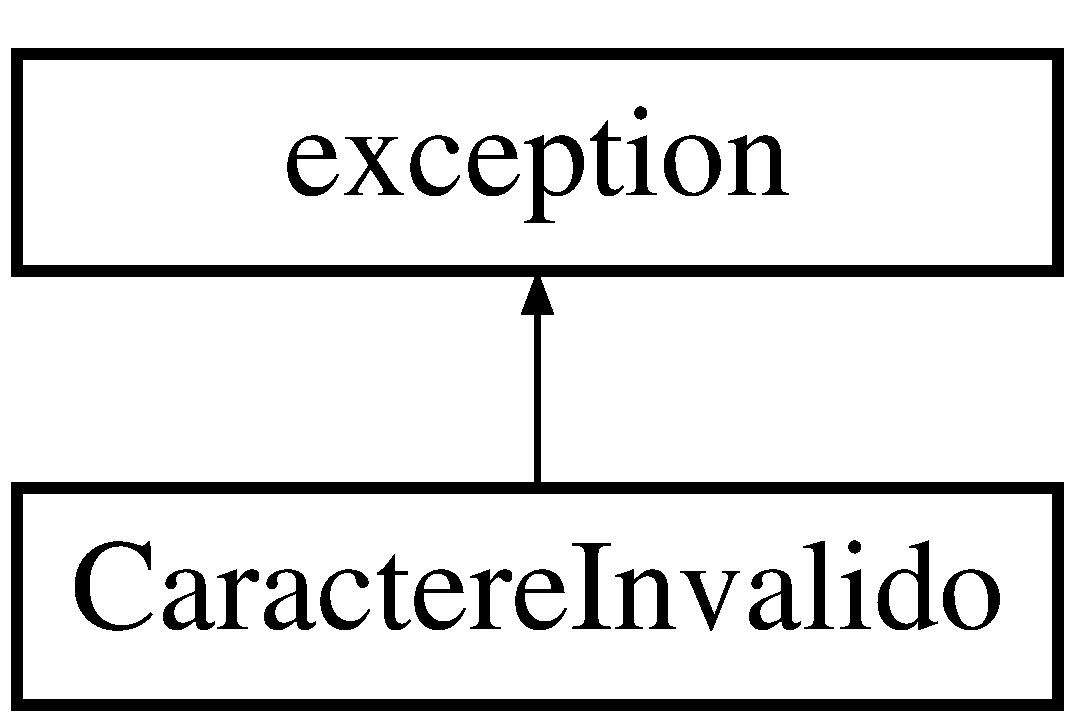
\includegraphics[height=2.000000cm]{classCaractereInvalido}
\end{center}
\end{figure}
\subsection*{Public Member Functions}
\begin{DoxyCompactItemize}
\item 
const char $\ast$ \hyperlink{classCaractereInvalido_afc8dae97f51348abe6909bd97d5959fb}{what} () const noexcept override
\end{DoxyCompactItemize}
\subsection*{Private Attributes}
\begin{DoxyCompactItemize}
\item 
string \hyperlink{classCaractereInvalido_ad7722f62c4ddc09838c94ef06d540780}{mensagem} = \char`\"{}Nome de usuário inválido. Tente novamente.\char`\"{}
\end{DoxyCompactItemize}


\subsection{Member Function Documentation}
\mbox{\Hypertarget{classCaractereInvalido_afc8dae97f51348abe6909bd97d5959fb}\label{classCaractereInvalido_afc8dae97f51348abe6909bd97d5959fb}} 
\index{Caractere\+Invalido@{Caractere\+Invalido}!what@{what}}
\index{what@{what}!Caractere\+Invalido@{Caractere\+Invalido}}
\subsubsection{\texorpdfstring{what()}{what()}}
{\footnotesize\ttfamily const char$\ast$ Caractere\+Invalido\+::what (\begin{DoxyParamCaption}{ }\end{DoxyParamCaption}) const\hspace{0.3cm}{\ttfamily [inline]}, {\ttfamily [override]}, {\ttfamily [noexcept]}}



\subsection{Member Data Documentation}
\mbox{\Hypertarget{classCaractereInvalido_ad7722f62c4ddc09838c94ef06d540780}\label{classCaractereInvalido_ad7722f62c4ddc09838c94ef06d540780}} 
\index{Caractere\+Invalido@{Caractere\+Invalido}!mensagem@{mensagem}}
\index{mensagem@{mensagem}!Caractere\+Invalido@{Caractere\+Invalido}}
\subsubsection{\texorpdfstring{mensagem}{mensagem}}
{\footnotesize\ttfamily string Caractere\+Invalido\+::mensagem = \char`\"{}Nome de usuário inválido. Tente novamente.\char`\"{}\hspace{0.3cm}{\ttfamily [private]}}



The documentation for this class was generated from the following file\+:\begin{DoxyCompactItemize}
\item 
include/excecoes/\hyperlink{exc__usuario_8hpp}{exc\+\_\+usuario.\+hpp}\end{DoxyCompactItemize}

\hypertarget{classComandoEditarGrupoErrado}{}\section{Comando\+Editar\+Grupo\+Errado Class Reference}
\label{classComandoEditarGrupoErrado}\index{Comando\+Editar\+Grupo\+Errado@{Comando\+Editar\+Grupo\+Errado}}


{\ttfamily \#include $<$exc\+\_\+comando.\+hpp$>$}

Inheritance diagram for Comando\+Editar\+Grupo\+Errado\+:\begin{figure}[H]
\begin{center}
\leavevmode
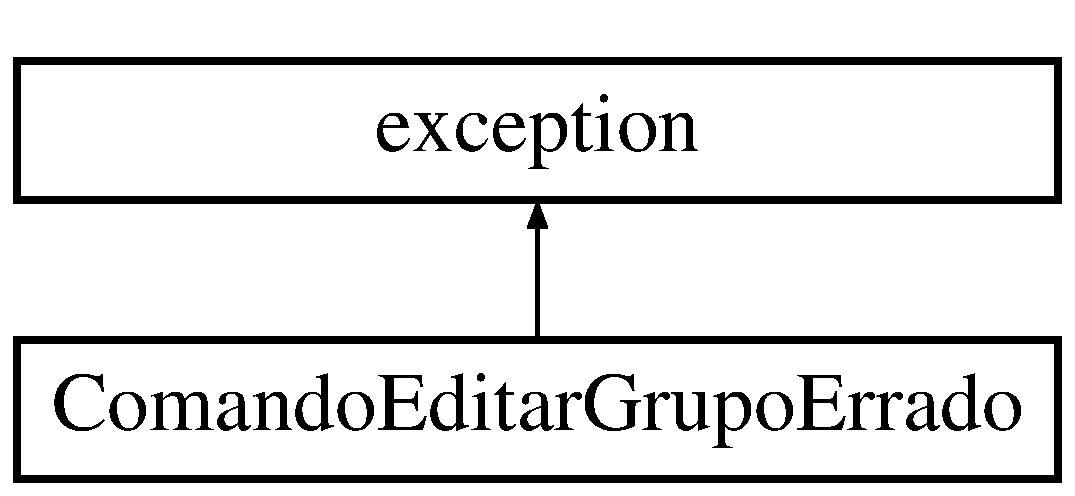
\includegraphics[height=2.000000cm]{classComandoEditarGrupoErrado}
\end{center}
\end{figure}
\subsection*{Public Member Functions}
\begin{DoxyCompactItemize}
\item 
const char $\ast$ \hyperlink{classComandoEditarGrupoErrado_a76dd1929368b3b0d0cc1443cd5a98bb6}{what} () const noexcept override
\end{DoxyCompactItemize}
\subsection*{Private Attributes}
\begin{DoxyCompactItemize}
\item 
string \hyperlink{classComandoEditarGrupoErrado_a9055ba079abfac17438aece597eb90d8}{mensagem} = \char`\"{}Você deve informar o ID do grupo que deseja editar. Tente novamente\char`\"{}
\end{DoxyCompactItemize}


\subsection{Member Function Documentation}
\mbox{\Hypertarget{classComandoEditarGrupoErrado_a76dd1929368b3b0d0cc1443cd5a98bb6}\label{classComandoEditarGrupoErrado_a76dd1929368b3b0d0cc1443cd5a98bb6}} 
\index{Comando\+Editar\+Grupo\+Errado@{Comando\+Editar\+Grupo\+Errado}!what@{what}}
\index{what@{what}!Comando\+Editar\+Grupo\+Errado@{Comando\+Editar\+Grupo\+Errado}}
\subsubsection{\texorpdfstring{what()}{what()}}
{\footnotesize\ttfamily const char$\ast$ Comando\+Editar\+Grupo\+Errado\+::what (\begin{DoxyParamCaption}{ }\end{DoxyParamCaption}) const\hspace{0.3cm}{\ttfamily [inline]}, {\ttfamily [override]}, {\ttfamily [noexcept]}}



\subsection{Member Data Documentation}
\mbox{\Hypertarget{classComandoEditarGrupoErrado_a9055ba079abfac17438aece597eb90d8}\label{classComandoEditarGrupoErrado_a9055ba079abfac17438aece597eb90d8}} 
\index{Comando\+Editar\+Grupo\+Errado@{Comando\+Editar\+Grupo\+Errado}!mensagem@{mensagem}}
\index{mensagem@{mensagem}!Comando\+Editar\+Grupo\+Errado@{Comando\+Editar\+Grupo\+Errado}}
\subsubsection{\texorpdfstring{mensagem}{mensagem}}
{\footnotesize\ttfamily string Comando\+Editar\+Grupo\+Errado\+::mensagem = \char`\"{}Você deve informar o ID do grupo que deseja editar. Tente novamente\char`\"{}\hspace{0.3cm}{\ttfamily [private]}}



The documentation for this class was generated from the following file\+:\begin{DoxyCompactItemize}
\item 
include/excecoes/\hyperlink{exc__comando_8hpp}{exc\+\_\+comando.\+hpp}\end{DoxyCompactItemize}

\hypertarget{classComandoEditarPrioridadeErrado}{}\section{Comando\+Editar\+Prioridade\+Errado Class Reference}
\label{classComandoEditarPrioridadeErrado}\index{Comando\+Editar\+Prioridade\+Errado@{Comando\+Editar\+Prioridade\+Errado}}


{\ttfamily \#include $<$exc\+\_\+comando.\+hpp$>$}

Inheritance diagram for Comando\+Editar\+Prioridade\+Errado\+:\begin{figure}[H]
\begin{center}
\leavevmode
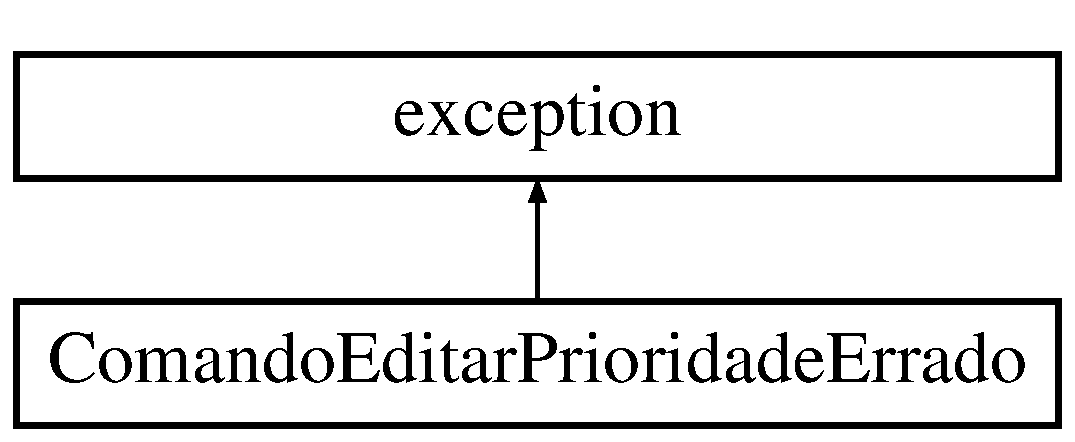
\includegraphics[height=2.000000cm]{classComandoEditarPrioridadeErrado}
\end{center}
\end{figure}
\subsection*{Public Member Functions}
\begin{DoxyCompactItemize}
\item 
const char $\ast$ \hyperlink{classComandoEditarPrioridadeErrado_a03d338a6103abdc73ce0c8554543c9d9}{what} () const noexcept override
\end{DoxyCompactItemize}
\subsection*{Private Attributes}
\begin{DoxyCompactItemize}
\item 
string \hyperlink{classComandoEditarPrioridadeErrado_a262cdc745b1bfc1d621b657a3c7c39ed}{mensagem} = \char`\"{}Você deve informar o ID da prioridade que deseja editar. Tente novamente\char`\"{}
\end{DoxyCompactItemize}


\subsection{Member Function Documentation}
\mbox{\Hypertarget{classComandoEditarPrioridadeErrado_a03d338a6103abdc73ce0c8554543c9d9}\label{classComandoEditarPrioridadeErrado_a03d338a6103abdc73ce0c8554543c9d9}} 
\index{Comando\+Editar\+Prioridade\+Errado@{Comando\+Editar\+Prioridade\+Errado}!what@{what}}
\index{what@{what}!Comando\+Editar\+Prioridade\+Errado@{Comando\+Editar\+Prioridade\+Errado}}
\subsubsection{\texorpdfstring{what()}{what()}}
{\footnotesize\ttfamily const char$\ast$ Comando\+Editar\+Prioridade\+Errado\+::what (\begin{DoxyParamCaption}{ }\end{DoxyParamCaption}) const\hspace{0.3cm}{\ttfamily [inline]}, {\ttfamily [override]}, {\ttfamily [noexcept]}}



\subsection{Member Data Documentation}
\mbox{\Hypertarget{classComandoEditarPrioridadeErrado_a262cdc745b1bfc1d621b657a3c7c39ed}\label{classComandoEditarPrioridadeErrado_a262cdc745b1bfc1d621b657a3c7c39ed}} 
\index{Comando\+Editar\+Prioridade\+Errado@{Comando\+Editar\+Prioridade\+Errado}!mensagem@{mensagem}}
\index{mensagem@{mensagem}!Comando\+Editar\+Prioridade\+Errado@{Comando\+Editar\+Prioridade\+Errado}}
\subsubsection{\texorpdfstring{mensagem}{mensagem}}
{\footnotesize\ttfamily string Comando\+Editar\+Prioridade\+Errado\+::mensagem = \char`\"{}Você deve informar o ID da prioridade que deseja editar. Tente novamente\char`\"{}\hspace{0.3cm}{\ttfamily [private]}}



The documentation for this class was generated from the following file\+:\begin{DoxyCompactItemize}
\item 
include/excecoes/\hyperlink{exc__comando_8hpp}{exc\+\_\+comando.\+hpp}\end{DoxyCompactItemize}

\hypertarget{classComandoEditarTarefaErrado}{}\section{Comando\+Editar\+Tarefa\+Errado Class Reference}
\label{classComandoEditarTarefaErrado}\index{Comando\+Editar\+Tarefa\+Errado@{Comando\+Editar\+Tarefa\+Errado}}


{\ttfamily \#include $<$exc\+\_\+comando.\+hpp$>$}

Inheritance diagram for Comando\+Editar\+Tarefa\+Errado\+:\begin{figure}[H]
\begin{center}
\leavevmode
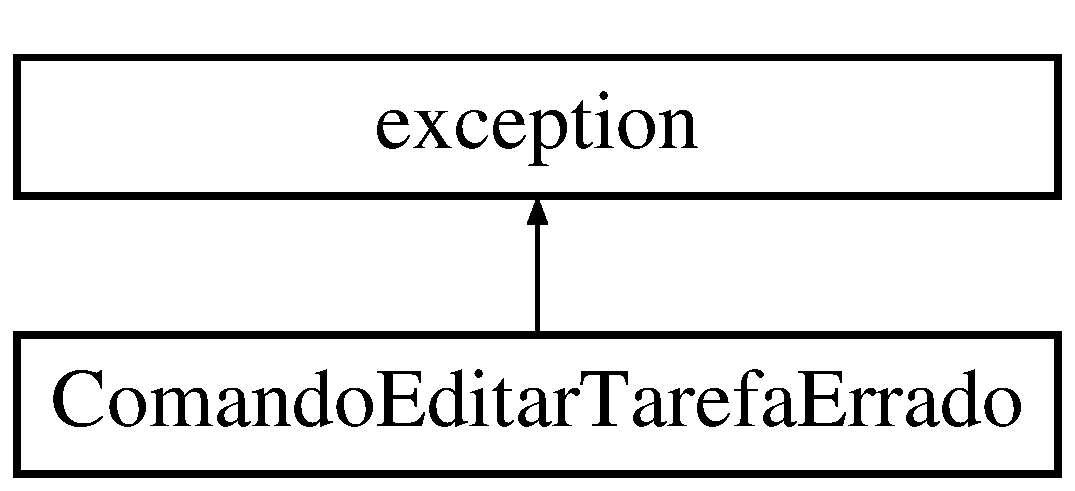
\includegraphics[height=2.000000cm]{classComandoEditarTarefaErrado}
\end{center}
\end{figure}
\subsection*{Public Member Functions}
\begin{DoxyCompactItemize}
\item 
const char $\ast$ \hyperlink{classComandoEditarTarefaErrado_aed17d6c56aea0b46eb88cff12ee5e25e}{what} () const noexcept override
\end{DoxyCompactItemize}
\subsection*{Private Attributes}
\begin{DoxyCompactItemize}
\item 
string \hyperlink{classComandoEditarTarefaErrado_a52e77fe112f01f71de548189720132c9}{mensagem} = \char`\"{}Você deve informar o ID da tarefa que deseja editar. Tente novamente\char`\"{}
\end{DoxyCompactItemize}


\subsection{Member Function Documentation}
\mbox{\Hypertarget{classComandoEditarTarefaErrado_aed17d6c56aea0b46eb88cff12ee5e25e}\label{classComandoEditarTarefaErrado_aed17d6c56aea0b46eb88cff12ee5e25e}} 
\index{Comando\+Editar\+Tarefa\+Errado@{Comando\+Editar\+Tarefa\+Errado}!what@{what}}
\index{what@{what}!Comando\+Editar\+Tarefa\+Errado@{Comando\+Editar\+Tarefa\+Errado}}
\subsubsection{\texorpdfstring{what()}{what()}}
{\footnotesize\ttfamily const char$\ast$ Comando\+Editar\+Tarefa\+Errado\+::what (\begin{DoxyParamCaption}{ }\end{DoxyParamCaption}) const\hspace{0.3cm}{\ttfamily [inline]}, {\ttfamily [override]}, {\ttfamily [noexcept]}}



\subsection{Member Data Documentation}
\mbox{\Hypertarget{classComandoEditarTarefaErrado_a52e77fe112f01f71de548189720132c9}\label{classComandoEditarTarefaErrado_a52e77fe112f01f71de548189720132c9}} 
\index{Comando\+Editar\+Tarefa\+Errado@{Comando\+Editar\+Tarefa\+Errado}!mensagem@{mensagem}}
\index{mensagem@{mensagem}!Comando\+Editar\+Tarefa\+Errado@{Comando\+Editar\+Tarefa\+Errado}}
\subsubsection{\texorpdfstring{mensagem}{mensagem}}
{\footnotesize\ttfamily string Comando\+Editar\+Tarefa\+Errado\+::mensagem = \char`\"{}Você deve informar o ID da tarefa que deseja editar. Tente novamente\char`\"{}\hspace{0.3cm}{\ttfamily [private]}}



The documentation for this class was generated from the following file\+:\begin{DoxyCompactItemize}
\item 
include/excecoes/\hyperlink{exc__comando_8hpp}{exc\+\_\+comando.\+hpp}\end{DoxyCompactItemize}

\hypertarget{classComandoExcluirGrupoErrado}{}\section{Comando\+Excluir\+Grupo\+Errado Class Reference}
\label{classComandoExcluirGrupoErrado}\index{Comando\+Excluir\+Grupo\+Errado@{Comando\+Excluir\+Grupo\+Errado}}


{\ttfamily \#include $<$exc\+\_\+comando.\+hpp$>$}

Inheritance diagram for Comando\+Excluir\+Grupo\+Errado\+:\begin{figure}[H]
\begin{center}
\leavevmode
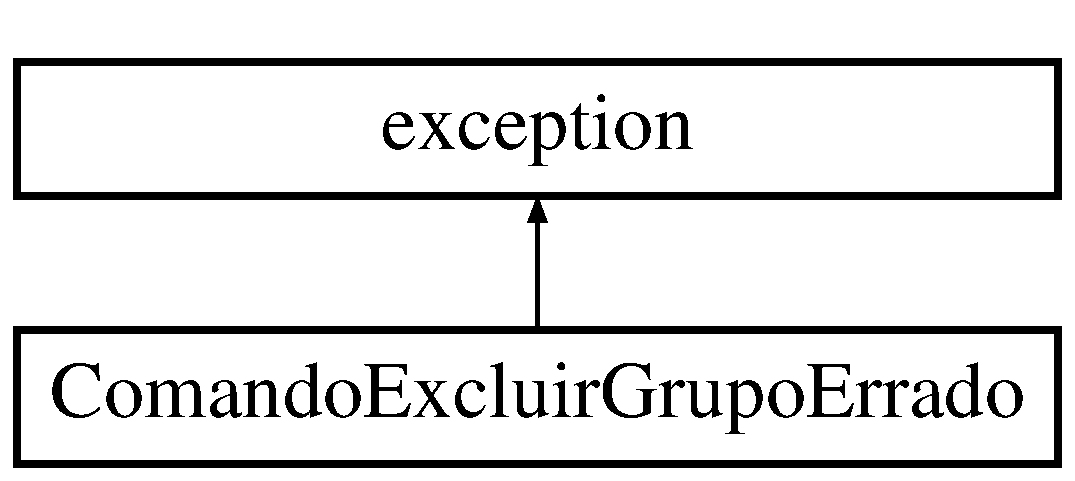
\includegraphics[height=2.000000cm]{classComandoExcluirGrupoErrado}
\end{center}
\end{figure}
\subsection*{Public Member Functions}
\begin{DoxyCompactItemize}
\item 
const char $\ast$ \hyperlink{classComandoExcluirGrupoErrado_abdf7deaa2a0467a556f57ed2d54b52d1}{what} () const noexcept override
\end{DoxyCompactItemize}
\subsection*{Private Attributes}
\begin{DoxyCompactItemize}
\item 
string \hyperlink{classComandoExcluirGrupoErrado_a3d55ba220737df2b3a454360ca1c7513}{mensagem} = \char`\"{}Você deve informar o ID do grupo que deseja editar. Tente novamente\char`\"{}
\end{DoxyCompactItemize}


\subsection{Member Function Documentation}
\mbox{\Hypertarget{classComandoExcluirGrupoErrado_abdf7deaa2a0467a556f57ed2d54b52d1}\label{classComandoExcluirGrupoErrado_abdf7deaa2a0467a556f57ed2d54b52d1}} 
\index{Comando\+Excluir\+Grupo\+Errado@{Comando\+Excluir\+Grupo\+Errado}!what@{what}}
\index{what@{what}!Comando\+Excluir\+Grupo\+Errado@{Comando\+Excluir\+Grupo\+Errado}}
\subsubsection{\texorpdfstring{what()}{what()}}
{\footnotesize\ttfamily const char$\ast$ Comando\+Excluir\+Grupo\+Errado\+::what (\begin{DoxyParamCaption}{ }\end{DoxyParamCaption}) const\hspace{0.3cm}{\ttfamily [inline]}, {\ttfamily [override]}, {\ttfamily [noexcept]}}



\subsection{Member Data Documentation}
\mbox{\Hypertarget{classComandoExcluirGrupoErrado_a3d55ba220737df2b3a454360ca1c7513}\label{classComandoExcluirGrupoErrado_a3d55ba220737df2b3a454360ca1c7513}} 
\index{Comando\+Excluir\+Grupo\+Errado@{Comando\+Excluir\+Grupo\+Errado}!mensagem@{mensagem}}
\index{mensagem@{mensagem}!Comando\+Excluir\+Grupo\+Errado@{Comando\+Excluir\+Grupo\+Errado}}
\subsubsection{\texorpdfstring{mensagem}{mensagem}}
{\footnotesize\ttfamily string Comando\+Excluir\+Grupo\+Errado\+::mensagem = \char`\"{}Você deve informar o ID do grupo que deseja editar. Tente novamente\char`\"{}\hspace{0.3cm}{\ttfamily [private]}}



The documentation for this class was generated from the following file\+:\begin{DoxyCompactItemize}
\item 
include/excecoes/\hyperlink{exc__comando_8hpp}{exc\+\_\+comando.\+hpp}\end{DoxyCompactItemize}

\hypertarget{classComandoExcluirPrioridadeErrado}{}\section{Comando\+Excluir\+Prioridade\+Errado Class Reference}
\label{classComandoExcluirPrioridadeErrado}\index{Comando\+Excluir\+Prioridade\+Errado@{Comando\+Excluir\+Prioridade\+Errado}}


{\ttfamily \#include $<$exc\+\_\+comando.\+hpp$>$}

Inheritance diagram for Comando\+Excluir\+Prioridade\+Errado\+:\begin{figure}[H]
\begin{center}
\leavevmode
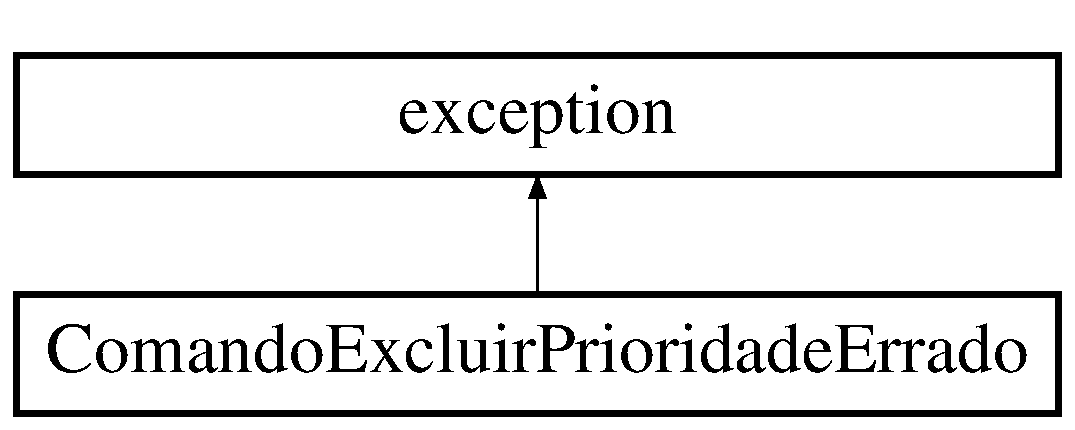
\includegraphics[height=2.000000cm]{classComandoExcluirPrioridadeErrado}
\end{center}
\end{figure}
\subsection*{Public Member Functions}
\begin{DoxyCompactItemize}
\item 
const char $\ast$ \hyperlink{classComandoExcluirPrioridadeErrado_a5cc6287358facad8209efc7c47eff853}{what} () const noexcept override
\end{DoxyCompactItemize}
\subsection*{Private Attributes}
\begin{DoxyCompactItemize}
\item 
string \hyperlink{classComandoExcluirPrioridadeErrado_a669931642bcb3157f9cdfc05bedff377}{mensagem} = \char`\"{}Você deve informar o ID da prioridade que deseja excluir. Tente novamente\char`\"{}
\end{DoxyCompactItemize}


\subsection{Member Function Documentation}
\mbox{\Hypertarget{classComandoExcluirPrioridadeErrado_a5cc6287358facad8209efc7c47eff853}\label{classComandoExcluirPrioridadeErrado_a5cc6287358facad8209efc7c47eff853}} 
\index{Comando\+Excluir\+Prioridade\+Errado@{Comando\+Excluir\+Prioridade\+Errado}!what@{what}}
\index{what@{what}!Comando\+Excluir\+Prioridade\+Errado@{Comando\+Excluir\+Prioridade\+Errado}}
\subsubsection{\texorpdfstring{what()}{what()}}
{\footnotesize\ttfamily const char$\ast$ Comando\+Excluir\+Prioridade\+Errado\+::what (\begin{DoxyParamCaption}{ }\end{DoxyParamCaption}) const\hspace{0.3cm}{\ttfamily [inline]}, {\ttfamily [override]}, {\ttfamily [noexcept]}}



\subsection{Member Data Documentation}
\mbox{\Hypertarget{classComandoExcluirPrioridadeErrado_a669931642bcb3157f9cdfc05bedff377}\label{classComandoExcluirPrioridadeErrado_a669931642bcb3157f9cdfc05bedff377}} 
\index{Comando\+Excluir\+Prioridade\+Errado@{Comando\+Excluir\+Prioridade\+Errado}!mensagem@{mensagem}}
\index{mensagem@{mensagem}!Comando\+Excluir\+Prioridade\+Errado@{Comando\+Excluir\+Prioridade\+Errado}}
\subsubsection{\texorpdfstring{mensagem}{mensagem}}
{\footnotesize\ttfamily string Comando\+Excluir\+Prioridade\+Errado\+::mensagem = \char`\"{}Você deve informar o ID da prioridade que deseja excluir. Tente novamente\char`\"{}\hspace{0.3cm}{\ttfamily [private]}}



The documentation for this class was generated from the following file\+:\begin{DoxyCompactItemize}
\item 
include/excecoes/\hyperlink{exc__comando_8hpp}{exc\+\_\+comando.\+hpp}\end{DoxyCompactItemize}

\hypertarget{classComandoExcluirTarefaErrado}{}\section{Comando\+Excluir\+Tarefa\+Errado Class Reference}
\label{classComandoExcluirTarefaErrado}\index{Comando\+Excluir\+Tarefa\+Errado@{Comando\+Excluir\+Tarefa\+Errado}}


{\ttfamily \#include $<$exc\+\_\+comando.\+hpp$>$}

Inheritance diagram for Comando\+Excluir\+Tarefa\+Errado\+:\begin{figure}[H]
\begin{center}
\leavevmode
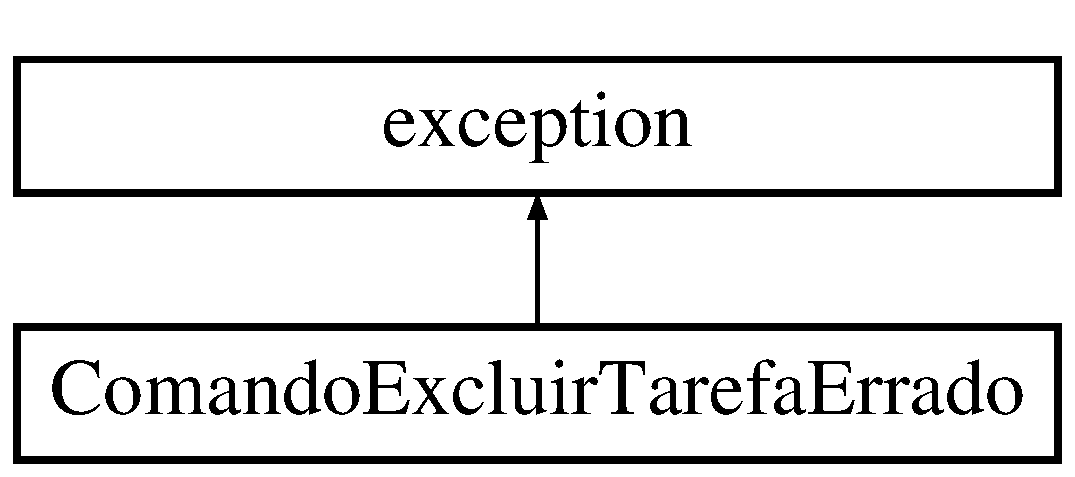
\includegraphics[height=2.000000cm]{classComandoExcluirTarefaErrado}
\end{center}
\end{figure}
\subsection*{Public Member Functions}
\begin{DoxyCompactItemize}
\item 
const char $\ast$ \hyperlink{classComandoExcluirTarefaErrado_a0e01ae298b6026f2497055d82f5b868f}{what} () const noexcept override
\end{DoxyCompactItemize}
\subsection*{Private Attributes}
\begin{DoxyCompactItemize}
\item 
string \hyperlink{classComandoExcluirTarefaErrado_a0223bc12d367ca404bab4ec1f5a084cf}{mensagem} = \char`\"{}Você deve informar o ID da tarefa que deseja excluir. Tente novamente\char`\"{}
\end{DoxyCompactItemize}


\subsection{Member Function Documentation}
\mbox{\Hypertarget{classComandoExcluirTarefaErrado_a0e01ae298b6026f2497055d82f5b868f}\label{classComandoExcluirTarefaErrado_a0e01ae298b6026f2497055d82f5b868f}} 
\index{Comando\+Excluir\+Tarefa\+Errado@{Comando\+Excluir\+Tarefa\+Errado}!what@{what}}
\index{what@{what}!Comando\+Excluir\+Tarefa\+Errado@{Comando\+Excluir\+Tarefa\+Errado}}
\subsubsection{\texorpdfstring{what()}{what()}}
{\footnotesize\ttfamily const char$\ast$ Comando\+Excluir\+Tarefa\+Errado\+::what (\begin{DoxyParamCaption}{ }\end{DoxyParamCaption}) const\hspace{0.3cm}{\ttfamily [inline]}, {\ttfamily [override]}, {\ttfamily [noexcept]}}



\subsection{Member Data Documentation}
\mbox{\Hypertarget{classComandoExcluirTarefaErrado_a0223bc12d367ca404bab4ec1f5a084cf}\label{classComandoExcluirTarefaErrado_a0223bc12d367ca404bab4ec1f5a084cf}} 
\index{Comando\+Excluir\+Tarefa\+Errado@{Comando\+Excluir\+Tarefa\+Errado}!mensagem@{mensagem}}
\index{mensagem@{mensagem}!Comando\+Excluir\+Tarefa\+Errado@{Comando\+Excluir\+Tarefa\+Errado}}
\subsubsection{\texorpdfstring{mensagem}{mensagem}}
{\footnotesize\ttfamily string Comando\+Excluir\+Tarefa\+Errado\+::mensagem = \char`\"{}Você deve informar o ID da tarefa que deseja excluir. Tente novamente\char`\"{}\hspace{0.3cm}{\ttfamily [private]}}



The documentation for this class was generated from the following file\+:\begin{DoxyCompactItemize}
\item 
include/excecoes/\hyperlink{exc__comando_8hpp}{exc\+\_\+comando.\+hpp}\end{DoxyCompactItemize}

\hypertarget{classComandoExibirTarefaErrado}{}\section{Comando\+Exibir\+Tarefa\+Errado Class Reference}
\label{classComandoExibirTarefaErrado}\index{Comando\+Exibir\+Tarefa\+Errado@{Comando\+Exibir\+Tarefa\+Errado}}


{\ttfamily \#include $<$exc\+\_\+comando.\+hpp$>$}

Inheritance diagram for Comando\+Exibir\+Tarefa\+Errado\+:\begin{figure}[H]
\begin{center}
\leavevmode
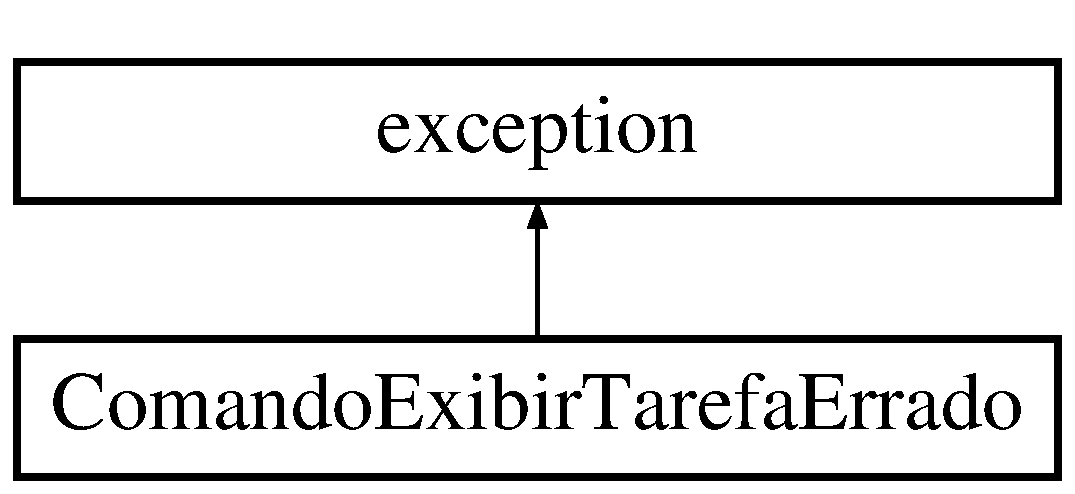
\includegraphics[height=2.000000cm]{classComandoExibirTarefaErrado}
\end{center}
\end{figure}
\subsection*{Public Member Functions}
\begin{DoxyCompactItemize}
\item 
const char $\ast$ \hyperlink{classComandoExibirTarefaErrado_abb4fbf8c6ce9ac105ab15000712a39ed}{what} () const noexcept override
\end{DoxyCompactItemize}
\subsection*{Private Attributes}
\begin{DoxyCompactItemize}
\item 
string \hyperlink{classComandoExibirTarefaErrado_ae5e55f9c70c2f3a187b86ecc32ca27dd}{mensagem} = \char`\"{}Você deve informar o ID da tarefa que deseja exibir. Tente novamente\char`\"{}
\end{DoxyCompactItemize}


\subsection{Member Function Documentation}
\mbox{\Hypertarget{classComandoExibirTarefaErrado_abb4fbf8c6ce9ac105ab15000712a39ed}\label{classComandoExibirTarefaErrado_abb4fbf8c6ce9ac105ab15000712a39ed}} 
\index{Comando\+Exibir\+Tarefa\+Errado@{Comando\+Exibir\+Tarefa\+Errado}!what@{what}}
\index{what@{what}!Comando\+Exibir\+Tarefa\+Errado@{Comando\+Exibir\+Tarefa\+Errado}}
\subsubsection{\texorpdfstring{what()}{what()}}
{\footnotesize\ttfamily const char$\ast$ Comando\+Exibir\+Tarefa\+Errado\+::what (\begin{DoxyParamCaption}{ }\end{DoxyParamCaption}) const\hspace{0.3cm}{\ttfamily [inline]}, {\ttfamily [override]}, {\ttfamily [noexcept]}}



\subsection{Member Data Documentation}
\mbox{\Hypertarget{classComandoExibirTarefaErrado_ae5e55f9c70c2f3a187b86ecc32ca27dd}\label{classComandoExibirTarefaErrado_ae5e55f9c70c2f3a187b86ecc32ca27dd}} 
\index{Comando\+Exibir\+Tarefa\+Errado@{Comando\+Exibir\+Tarefa\+Errado}!mensagem@{mensagem}}
\index{mensagem@{mensagem}!Comando\+Exibir\+Tarefa\+Errado@{Comando\+Exibir\+Tarefa\+Errado}}
\subsubsection{\texorpdfstring{mensagem}{mensagem}}
{\footnotesize\ttfamily string Comando\+Exibir\+Tarefa\+Errado\+::mensagem = \char`\"{}Você deve informar o ID da tarefa que deseja exibir. Tente novamente\char`\"{}\hspace{0.3cm}{\ttfamily [private]}}



The documentation for this class was generated from the following file\+:\begin{DoxyCompactItemize}
\item 
include/excecoes/\hyperlink{exc__comando_8hpp}{exc\+\_\+comando.\+hpp}\end{DoxyCompactItemize}

\hypertarget{classCriacaoGrupoCancelada}{}\section{Criacao\+Grupo\+Cancelada Class Reference}
\label{classCriacaoGrupoCancelada}\index{Criacao\+Grupo\+Cancelada@{Criacao\+Grupo\+Cancelada}}


{\ttfamily \#include $<$exc\+\_\+cancelamento.\+hpp$>$}

Inheritance diagram for Criacao\+Grupo\+Cancelada\+:\begin{figure}[H]
\begin{center}
\leavevmode
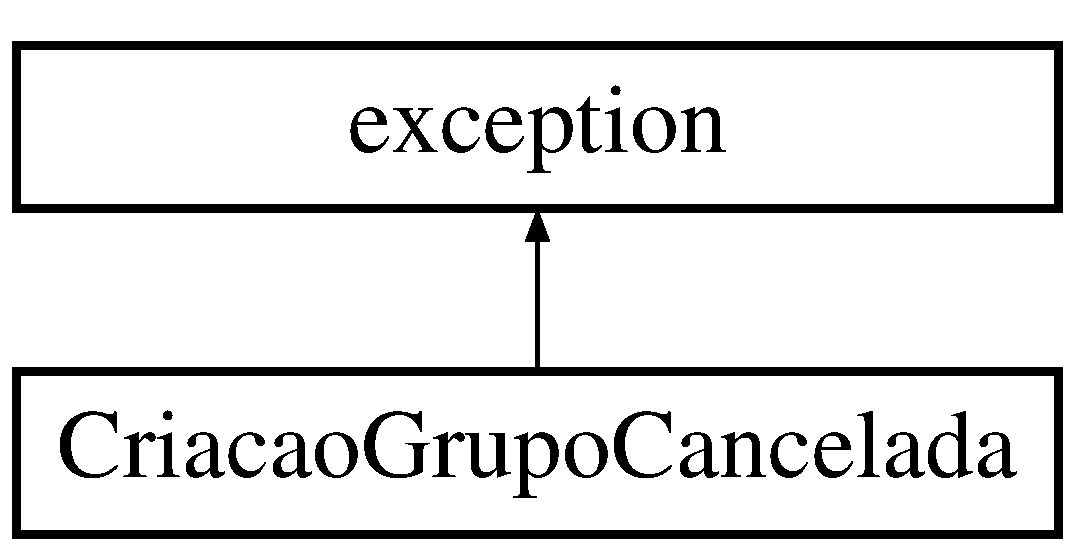
\includegraphics[height=2.000000cm]{classCriacaoGrupoCancelada}
\end{center}
\end{figure}
\subsection*{Public Member Functions}
\begin{DoxyCompactItemize}
\item 
const char $\ast$ \hyperlink{classCriacaoGrupoCancelada_a8e4b402896878ae2f154008d2e5eb136}{what} () const noexcept override
\end{DoxyCompactItemize}
\subsection*{Private Attributes}
\begin{DoxyCompactItemize}
\item 
string \hyperlink{classCriacaoGrupoCancelada_a4077c2d32782e91f124566a7085b4acf}{mensagem} = \char`\"{}Criação de grupo cancelada\char`\"{}
\end{DoxyCompactItemize}


\subsection{Member Function Documentation}
\mbox{\Hypertarget{classCriacaoGrupoCancelada_a8e4b402896878ae2f154008d2e5eb136}\label{classCriacaoGrupoCancelada_a8e4b402896878ae2f154008d2e5eb136}} 
\index{Criacao\+Grupo\+Cancelada@{Criacao\+Grupo\+Cancelada}!what@{what}}
\index{what@{what}!Criacao\+Grupo\+Cancelada@{Criacao\+Grupo\+Cancelada}}
\subsubsection{\texorpdfstring{what()}{what()}}
{\footnotesize\ttfamily const char$\ast$ Criacao\+Grupo\+Cancelada\+::what (\begin{DoxyParamCaption}{ }\end{DoxyParamCaption}) const\hspace{0.3cm}{\ttfamily [inline]}, {\ttfamily [override]}, {\ttfamily [noexcept]}}



\subsection{Member Data Documentation}
\mbox{\Hypertarget{classCriacaoGrupoCancelada_a4077c2d32782e91f124566a7085b4acf}\label{classCriacaoGrupoCancelada_a4077c2d32782e91f124566a7085b4acf}} 
\index{Criacao\+Grupo\+Cancelada@{Criacao\+Grupo\+Cancelada}!mensagem@{mensagem}}
\index{mensagem@{mensagem}!Criacao\+Grupo\+Cancelada@{Criacao\+Grupo\+Cancelada}}
\subsubsection{\texorpdfstring{mensagem}{mensagem}}
{\footnotesize\ttfamily string Criacao\+Grupo\+Cancelada\+::mensagem = \char`\"{}Criação de grupo cancelada\char`\"{}\hspace{0.3cm}{\ttfamily [private]}}



The documentation for this class was generated from the following file\+:\begin{DoxyCompactItemize}
\item 
include/excecoes/\hyperlink{exc__cancelamento_8hpp}{exc\+\_\+cancelamento.\+hpp}\end{DoxyCompactItemize}

\hypertarget{classCriacaoPrioridadeCancelada}{}\section{Criacao\+Prioridade\+Cancelada Class Reference}
\label{classCriacaoPrioridadeCancelada}\index{Criacao\+Prioridade\+Cancelada@{Criacao\+Prioridade\+Cancelada}}


{\ttfamily \#include $<$exc\+\_\+cancelamento.\+hpp$>$}

Inheritance diagram for Criacao\+Prioridade\+Cancelada\+:\begin{figure}[H]
\begin{center}
\leavevmode
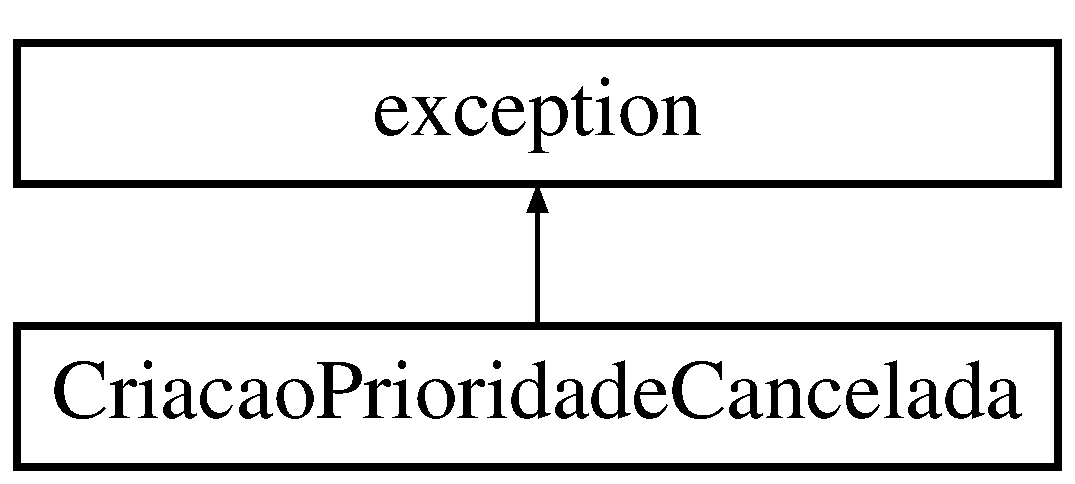
\includegraphics[height=2.000000cm]{classCriacaoPrioridadeCancelada}
\end{center}
\end{figure}
\subsection*{Public Member Functions}
\begin{DoxyCompactItemize}
\item 
const char $\ast$ \hyperlink{classCriacaoPrioridadeCancelada_aaa4835bad23542e67d2dedd75c9e7ded}{what} () const noexcept override
\end{DoxyCompactItemize}
\subsection*{Private Attributes}
\begin{DoxyCompactItemize}
\item 
string \hyperlink{classCriacaoPrioridadeCancelada_aec9dedf305887e4227ed1af5cf26b49c}{mensagem} = \char`\"{}Criação de prioridade cancelada\char`\"{}
\end{DoxyCompactItemize}


\subsection{Member Function Documentation}
\mbox{\Hypertarget{classCriacaoPrioridadeCancelada_aaa4835bad23542e67d2dedd75c9e7ded}\label{classCriacaoPrioridadeCancelada_aaa4835bad23542e67d2dedd75c9e7ded}} 
\index{Criacao\+Prioridade\+Cancelada@{Criacao\+Prioridade\+Cancelada}!what@{what}}
\index{what@{what}!Criacao\+Prioridade\+Cancelada@{Criacao\+Prioridade\+Cancelada}}
\subsubsection{\texorpdfstring{what()}{what()}}
{\footnotesize\ttfamily const char$\ast$ Criacao\+Prioridade\+Cancelada\+::what (\begin{DoxyParamCaption}{ }\end{DoxyParamCaption}) const\hspace{0.3cm}{\ttfamily [inline]}, {\ttfamily [override]}, {\ttfamily [noexcept]}}



\subsection{Member Data Documentation}
\mbox{\Hypertarget{classCriacaoPrioridadeCancelada_aec9dedf305887e4227ed1af5cf26b49c}\label{classCriacaoPrioridadeCancelada_aec9dedf305887e4227ed1af5cf26b49c}} 
\index{Criacao\+Prioridade\+Cancelada@{Criacao\+Prioridade\+Cancelada}!mensagem@{mensagem}}
\index{mensagem@{mensagem}!Criacao\+Prioridade\+Cancelada@{Criacao\+Prioridade\+Cancelada}}
\subsubsection{\texorpdfstring{mensagem}{mensagem}}
{\footnotesize\ttfamily string Criacao\+Prioridade\+Cancelada\+::mensagem = \char`\"{}Criação de prioridade cancelada\char`\"{}\hspace{0.3cm}{\ttfamily [private]}}



The documentation for this class was generated from the following file\+:\begin{DoxyCompactItemize}
\item 
include/excecoes/\hyperlink{exc__cancelamento_8hpp}{exc\+\_\+cancelamento.\+hpp}\end{DoxyCompactItemize}

\hypertarget{classCriacaoTarefaCancelada}{}\section{Criacao\+Tarefa\+Cancelada Class Reference}
\label{classCriacaoTarefaCancelada}\index{Criacao\+Tarefa\+Cancelada@{Criacao\+Tarefa\+Cancelada}}


{\ttfamily \#include $<$exc\+\_\+cancelamento.\+hpp$>$}

Inheritance diagram for Criacao\+Tarefa\+Cancelada\+:\begin{figure}[H]
\begin{center}
\leavevmode
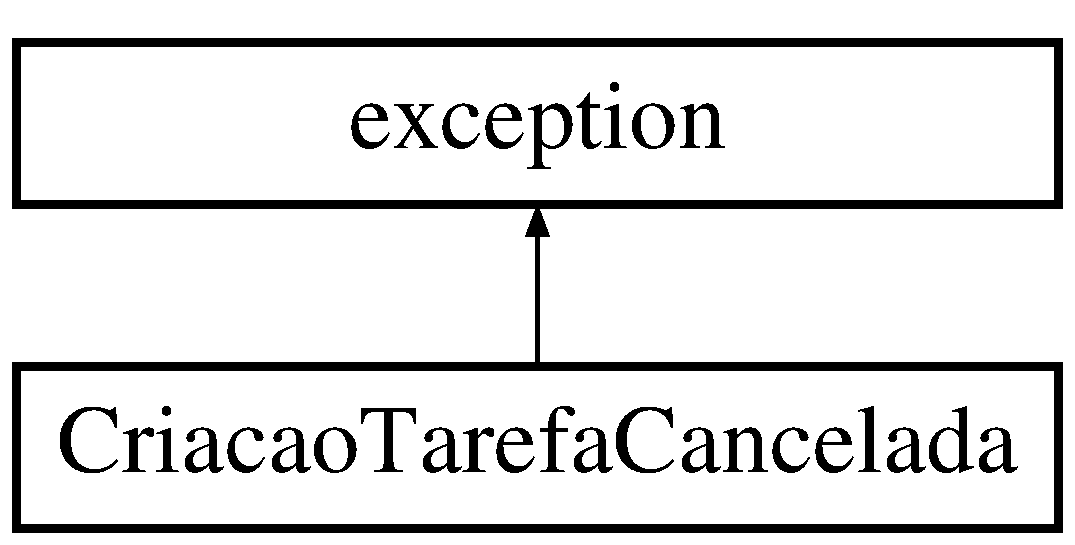
\includegraphics[height=2.000000cm]{classCriacaoTarefaCancelada}
\end{center}
\end{figure}
\subsection*{Public Member Functions}
\begin{DoxyCompactItemize}
\item 
const char $\ast$ \hyperlink{classCriacaoTarefaCancelada_aad818f5b62b134079ed47908825d52c9}{what} () const noexcept override
\end{DoxyCompactItemize}
\subsection*{Private Attributes}
\begin{DoxyCompactItemize}
\item 
string \hyperlink{classCriacaoTarefaCancelada_a8c861f898009f0691f033ecf83f4351f}{mensagem} = \char`\"{}Criação de tarefa cancelada\char`\"{}
\end{DoxyCompactItemize}


\subsection{Member Function Documentation}
\mbox{\Hypertarget{classCriacaoTarefaCancelada_aad818f5b62b134079ed47908825d52c9}\label{classCriacaoTarefaCancelada_aad818f5b62b134079ed47908825d52c9}} 
\index{Criacao\+Tarefa\+Cancelada@{Criacao\+Tarefa\+Cancelada}!what@{what}}
\index{what@{what}!Criacao\+Tarefa\+Cancelada@{Criacao\+Tarefa\+Cancelada}}
\subsubsection{\texorpdfstring{what()}{what()}}
{\footnotesize\ttfamily const char$\ast$ Criacao\+Tarefa\+Cancelada\+::what (\begin{DoxyParamCaption}{ }\end{DoxyParamCaption}) const\hspace{0.3cm}{\ttfamily [inline]}, {\ttfamily [override]}, {\ttfamily [noexcept]}}



\subsection{Member Data Documentation}
\mbox{\Hypertarget{classCriacaoTarefaCancelada_a8c861f898009f0691f033ecf83f4351f}\label{classCriacaoTarefaCancelada_a8c861f898009f0691f033ecf83f4351f}} 
\index{Criacao\+Tarefa\+Cancelada@{Criacao\+Tarefa\+Cancelada}!mensagem@{mensagem}}
\index{mensagem@{mensagem}!Criacao\+Tarefa\+Cancelada@{Criacao\+Tarefa\+Cancelada}}
\subsubsection{\texorpdfstring{mensagem}{mensagem}}
{\footnotesize\ttfamily string Criacao\+Tarefa\+Cancelada\+::mensagem = \char`\"{}Criação de tarefa cancelada\char`\"{}\hspace{0.3cm}{\ttfamily [private]}}



The documentation for this class was generated from the following file\+:\begin{DoxyCompactItemize}
\item 
include/excecoes/\hyperlink{exc__cancelamento_8hpp}{exc\+\_\+cancelamento.\+hpp}\end{DoxyCompactItemize}

\hypertarget{classEdicaoGrupoCancelada}{}\section{Edicao\+Grupo\+Cancelada Class Reference}
\label{classEdicaoGrupoCancelada}\index{Edicao\+Grupo\+Cancelada@{Edicao\+Grupo\+Cancelada}}


{\ttfamily \#include $<$exc\+\_\+cancelamento.\+hpp$>$}

Inheritance diagram for Edicao\+Grupo\+Cancelada\+:\begin{figure}[H]
\begin{center}
\leavevmode
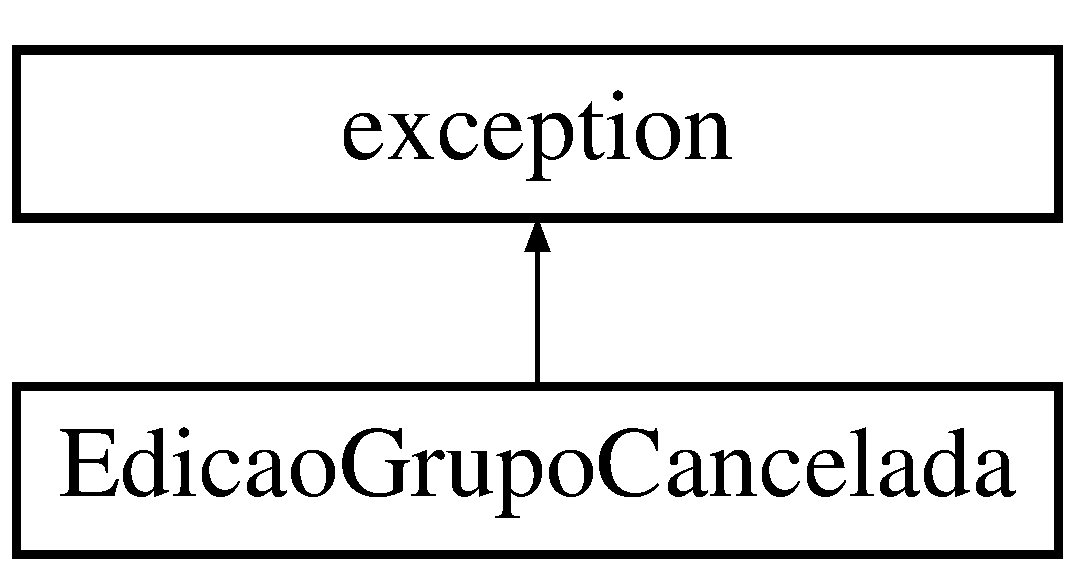
\includegraphics[height=2.000000cm]{classEdicaoGrupoCancelada}
\end{center}
\end{figure}
\subsection*{Public Member Functions}
\begin{DoxyCompactItemize}
\item 
const char $\ast$ \hyperlink{classEdicaoGrupoCancelada_a110bd7cb77b4df99d5a4dd051874ce19}{what} () const noexcept override
\end{DoxyCompactItemize}
\subsection*{Private Attributes}
\begin{DoxyCompactItemize}
\item 
string \hyperlink{classEdicaoGrupoCancelada_a53370c1e225786f8e874b8368468d793}{mensagem} = \char`\"{}Edição de grupo cancelada\char`\"{}
\end{DoxyCompactItemize}


\subsection{Member Function Documentation}
\mbox{\Hypertarget{classEdicaoGrupoCancelada_a110bd7cb77b4df99d5a4dd051874ce19}\label{classEdicaoGrupoCancelada_a110bd7cb77b4df99d5a4dd051874ce19}} 
\index{Edicao\+Grupo\+Cancelada@{Edicao\+Grupo\+Cancelada}!what@{what}}
\index{what@{what}!Edicao\+Grupo\+Cancelada@{Edicao\+Grupo\+Cancelada}}
\subsubsection{\texorpdfstring{what()}{what()}}
{\footnotesize\ttfamily const char$\ast$ Edicao\+Grupo\+Cancelada\+::what (\begin{DoxyParamCaption}{ }\end{DoxyParamCaption}) const\hspace{0.3cm}{\ttfamily [inline]}, {\ttfamily [override]}, {\ttfamily [noexcept]}}



\subsection{Member Data Documentation}
\mbox{\Hypertarget{classEdicaoGrupoCancelada_a53370c1e225786f8e874b8368468d793}\label{classEdicaoGrupoCancelada_a53370c1e225786f8e874b8368468d793}} 
\index{Edicao\+Grupo\+Cancelada@{Edicao\+Grupo\+Cancelada}!mensagem@{mensagem}}
\index{mensagem@{mensagem}!Edicao\+Grupo\+Cancelada@{Edicao\+Grupo\+Cancelada}}
\subsubsection{\texorpdfstring{mensagem}{mensagem}}
{\footnotesize\ttfamily string Edicao\+Grupo\+Cancelada\+::mensagem = \char`\"{}Edição de grupo cancelada\char`\"{}\hspace{0.3cm}{\ttfamily [private]}}



The documentation for this class was generated from the following file\+:\begin{DoxyCompactItemize}
\item 
include/excecoes/\hyperlink{exc__cancelamento_8hpp}{exc\+\_\+cancelamento.\+hpp}\end{DoxyCompactItemize}

\hypertarget{classEdicaoPrioridadeCancelada}{}\section{Edicao\+Prioridade\+Cancelada Class Reference}
\label{classEdicaoPrioridadeCancelada}\index{Edicao\+Prioridade\+Cancelada@{Edicao\+Prioridade\+Cancelada}}


{\ttfamily \#include $<$exc\+\_\+cancelamento.\+hpp$>$}

Inheritance diagram for Edicao\+Prioridade\+Cancelada\+:\begin{figure}[H]
\begin{center}
\leavevmode
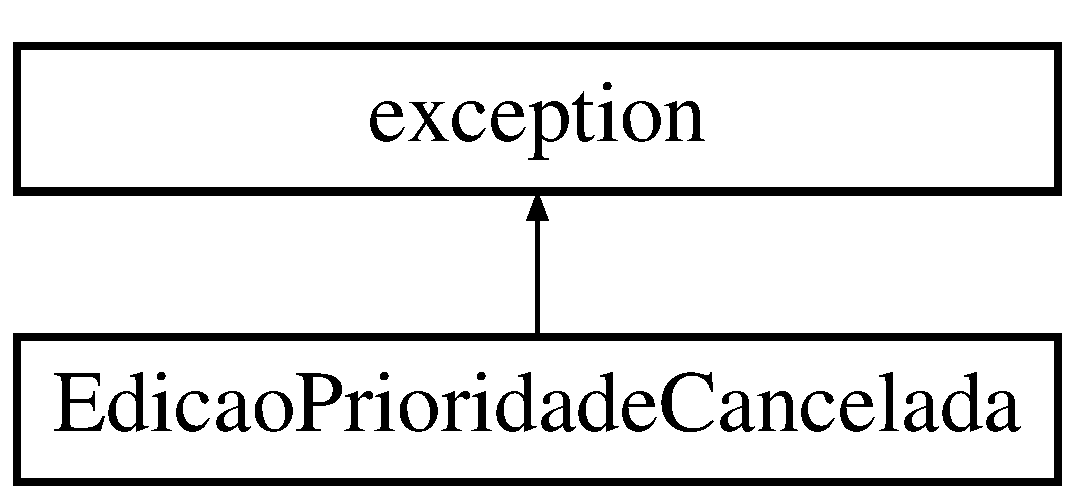
\includegraphics[height=2.000000cm]{classEdicaoPrioridadeCancelada}
\end{center}
\end{figure}
\subsection*{Public Member Functions}
\begin{DoxyCompactItemize}
\item 
const char $\ast$ \hyperlink{classEdicaoPrioridadeCancelada_a40a8af51b8b5e2c3c92b372e4c25edc3}{what} () const noexcept override
\end{DoxyCompactItemize}
\subsection*{Private Attributes}
\begin{DoxyCompactItemize}
\item 
string \hyperlink{classEdicaoPrioridadeCancelada_aa394e119ef20d94ce5ba0633dc0294d2}{mensagem} = \char`\"{}Edição de prioridade cancelada\char`\"{}
\end{DoxyCompactItemize}


\subsection{Member Function Documentation}
\mbox{\Hypertarget{classEdicaoPrioridadeCancelada_a40a8af51b8b5e2c3c92b372e4c25edc3}\label{classEdicaoPrioridadeCancelada_a40a8af51b8b5e2c3c92b372e4c25edc3}} 
\index{Edicao\+Prioridade\+Cancelada@{Edicao\+Prioridade\+Cancelada}!what@{what}}
\index{what@{what}!Edicao\+Prioridade\+Cancelada@{Edicao\+Prioridade\+Cancelada}}
\subsubsection{\texorpdfstring{what()}{what()}}
{\footnotesize\ttfamily const char$\ast$ Edicao\+Prioridade\+Cancelada\+::what (\begin{DoxyParamCaption}{ }\end{DoxyParamCaption}) const\hspace{0.3cm}{\ttfamily [inline]}, {\ttfamily [override]}, {\ttfamily [noexcept]}}



\subsection{Member Data Documentation}
\mbox{\Hypertarget{classEdicaoPrioridadeCancelada_aa394e119ef20d94ce5ba0633dc0294d2}\label{classEdicaoPrioridadeCancelada_aa394e119ef20d94ce5ba0633dc0294d2}} 
\index{Edicao\+Prioridade\+Cancelada@{Edicao\+Prioridade\+Cancelada}!mensagem@{mensagem}}
\index{mensagem@{mensagem}!Edicao\+Prioridade\+Cancelada@{Edicao\+Prioridade\+Cancelada}}
\subsubsection{\texorpdfstring{mensagem}{mensagem}}
{\footnotesize\ttfamily string Edicao\+Prioridade\+Cancelada\+::mensagem = \char`\"{}Edição de prioridade cancelada\char`\"{}\hspace{0.3cm}{\ttfamily [private]}}



The documentation for this class was generated from the following file\+:\begin{DoxyCompactItemize}
\item 
include/excecoes/\hyperlink{exc__cancelamento_8hpp}{exc\+\_\+cancelamento.\+hpp}\end{DoxyCompactItemize}

\hypertarget{classEdicaoTarefaCancelada}{}\section{Edicao\+Tarefa\+Cancelada Class Reference}
\label{classEdicaoTarefaCancelada}\index{Edicao\+Tarefa\+Cancelada@{Edicao\+Tarefa\+Cancelada}}


{\ttfamily \#include $<$exc\+\_\+cancelamento.\+hpp$>$}

Inheritance diagram for Edicao\+Tarefa\+Cancelada\+:\begin{figure}[H]
\begin{center}
\leavevmode
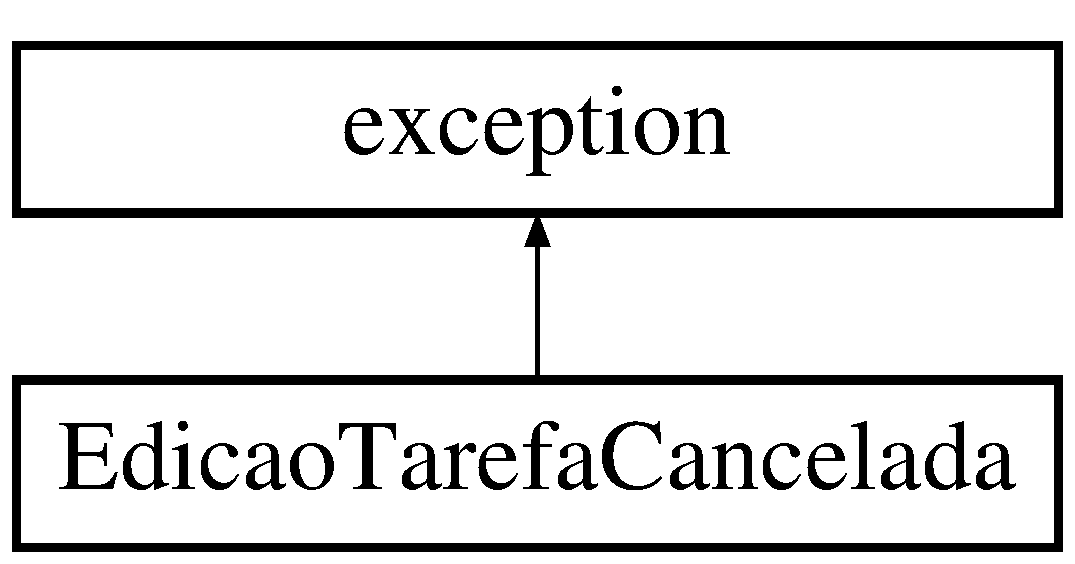
\includegraphics[height=2.000000cm]{classEdicaoTarefaCancelada}
\end{center}
\end{figure}
\subsection*{Public Member Functions}
\begin{DoxyCompactItemize}
\item 
const char $\ast$ \hyperlink{classEdicaoTarefaCancelada_a29a5052c938b209eddb78b9dc1200122}{what} () const noexcept override
\end{DoxyCompactItemize}
\subsection*{Private Attributes}
\begin{DoxyCompactItemize}
\item 
string \hyperlink{classEdicaoTarefaCancelada_a9b2145786ee5d1969d5f7703f6e4fb60}{mensagem} = \char`\"{}Edição de tarefa cancelada\char`\"{}
\end{DoxyCompactItemize}


\subsection{Member Function Documentation}
\mbox{\Hypertarget{classEdicaoTarefaCancelada_a29a5052c938b209eddb78b9dc1200122}\label{classEdicaoTarefaCancelada_a29a5052c938b209eddb78b9dc1200122}} 
\index{Edicao\+Tarefa\+Cancelada@{Edicao\+Tarefa\+Cancelada}!what@{what}}
\index{what@{what}!Edicao\+Tarefa\+Cancelada@{Edicao\+Tarefa\+Cancelada}}
\subsubsection{\texorpdfstring{what()}{what()}}
{\footnotesize\ttfamily const char$\ast$ Edicao\+Tarefa\+Cancelada\+::what (\begin{DoxyParamCaption}{ }\end{DoxyParamCaption}) const\hspace{0.3cm}{\ttfamily [inline]}, {\ttfamily [override]}, {\ttfamily [noexcept]}}



\subsection{Member Data Documentation}
\mbox{\Hypertarget{classEdicaoTarefaCancelada_a9b2145786ee5d1969d5f7703f6e4fb60}\label{classEdicaoTarefaCancelada_a9b2145786ee5d1969d5f7703f6e4fb60}} 
\index{Edicao\+Tarefa\+Cancelada@{Edicao\+Tarefa\+Cancelada}!mensagem@{mensagem}}
\index{mensagem@{mensagem}!Edicao\+Tarefa\+Cancelada@{Edicao\+Tarefa\+Cancelada}}
\subsubsection{\texorpdfstring{mensagem}{mensagem}}
{\footnotesize\ttfamily string Edicao\+Tarefa\+Cancelada\+::mensagem = \char`\"{}Edição de tarefa cancelada\char`\"{}\hspace{0.3cm}{\ttfamily [private]}}



The documentation for this class was generated from the following file\+:\begin{DoxyCompactItemize}
\item 
include/excecoes/\hyperlink{exc__cancelamento_8hpp}{exc\+\_\+cancelamento.\+hpp}\end{DoxyCompactItemize}

\hypertarget{classErroAoAbrirArquivo}{}\section{Erro\+Ao\+Abrir\+Arquivo Class Reference}
\label{classErroAoAbrirArquivo}\index{Erro\+Ao\+Abrir\+Arquivo@{Erro\+Ao\+Abrir\+Arquivo}}


{\ttfamily \#include $<$exc\+\_\+arquivo.\+hpp$>$}

Inheritance diagram for Erro\+Ao\+Abrir\+Arquivo\+:\begin{figure}[H]
\begin{center}
\leavevmode
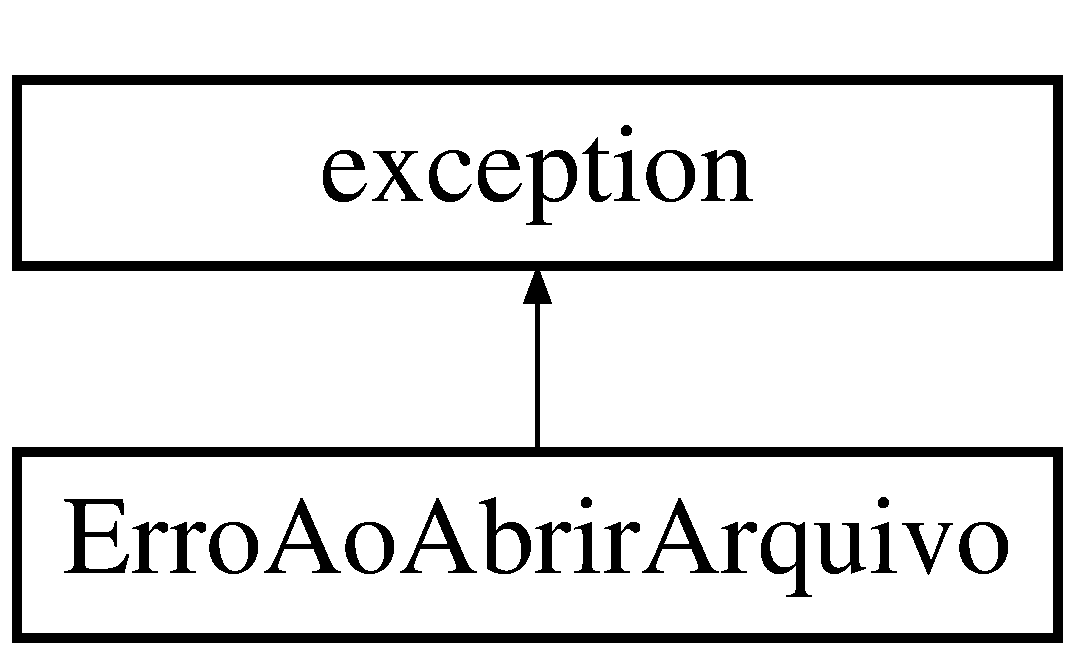
\includegraphics[height=2.000000cm]{classErroAoAbrirArquivo}
\end{center}
\end{figure}
\subsection*{Public Member Functions}
\begin{DoxyCompactItemize}
\item 
const char $\ast$ \hyperlink{classErroAoAbrirArquivo_a76820759458b6b1a6d89f2c685603ccd}{what} () const noexcept override
\end{DoxyCompactItemize}
\subsection*{Private Attributes}
\begin{DoxyCompactItemize}
\item 
string \hyperlink{classErroAoAbrirArquivo_a96c16ba42b2fbb0cfb8aed38801748f0}{mensagem} = \char`\"{}Erro ao abrir arquivo do usuário.\char`\"{}
\end{DoxyCompactItemize}


\subsection{Member Function Documentation}
\mbox{\Hypertarget{classErroAoAbrirArquivo_a76820759458b6b1a6d89f2c685603ccd}\label{classErroAoAbrirArquivo_a76820759458b6b1a6d89f2c685603ccd}} 
\index{Erro\+Ao\+Abrir\+Arquivo@{Erro\+Ao\+Abrir\+Arquivo}!what@{what}}
\index{what@{what}!Erro\+Ao\+Abrir\+Arquivo@{Erro\+Ao\+Abrir\+Arquivo}}
\subsubsection{\texorpdfstring{what()}{what()}}
{\footnotesize\ttfamily const char$\ast$ Erro\+Ao\+Abrir\+Arquivo\+::what (\begin{DoxyParamCaption}{ }\end{DoxyParamCaption}) const\hspace{0.3cm}{\ttfamily [inline]}, {\ttfamily [override]}, {\ttfamily [noexcept]}}



\subsection{Member Data Documentation}
\mbox{\Hypertarget{classErroAoAbrirArquivo_a96c16ba42b2fbb0cfb8aed38801748f0}\label{classErroAoAbrirArquivo_a96c16ba42b2fbb0cfb8aed38801748f0}} 
\index{Erro\+Ao\+Abrir\+Arquivo@{Erro\+Ao\+Abrir\+Arquivo}!mensagem@{mensagem}}
\index{mensagem@{mensagem}!Erro\+Ao\+Abrir\+Arquivo@{Erro\+Ao\+Abrir\+Arquivo}}
\subsubsection{\texorpdfstring{mensagem}{mensagem}}
{\footnotesize\ttfamily string Erro\+Ao\+Abrir\+Arquivo\+::mensagem = \char`\"{}Erro ao abrir arquivo do usuário.\char`\"{}\hspace{0.3cm}{\ttfamily [private]}}



The documentation for this class was generated from the following file\+:\begin{DoxyCompactItemize}
\item 
include/excecoes/\hyperlink{exc__arquivo_8hpp}{exc\+\_\+arquivo.\+hpp}\end{DoxyCompactItemize}

\hypertarget{classErroAoApagarGrupo}{}\section{Erro\+Ao\+Apagar\+Grupo Class Reference}
\label{classErroAoApagarGrupo}\index{Erro\+Ao\+Apagar\+Grupo@{Erro\+Ao\+Apagar\+Grupo}}


{\ttfamily \#include $<$exc\+\_\+grupo.\+hpp$>$}

Inheritance diagram for Erro\+Ao\+Apagar\+Grupo\+:\begin{figure}[H]
\begin{center}
\leavevmode
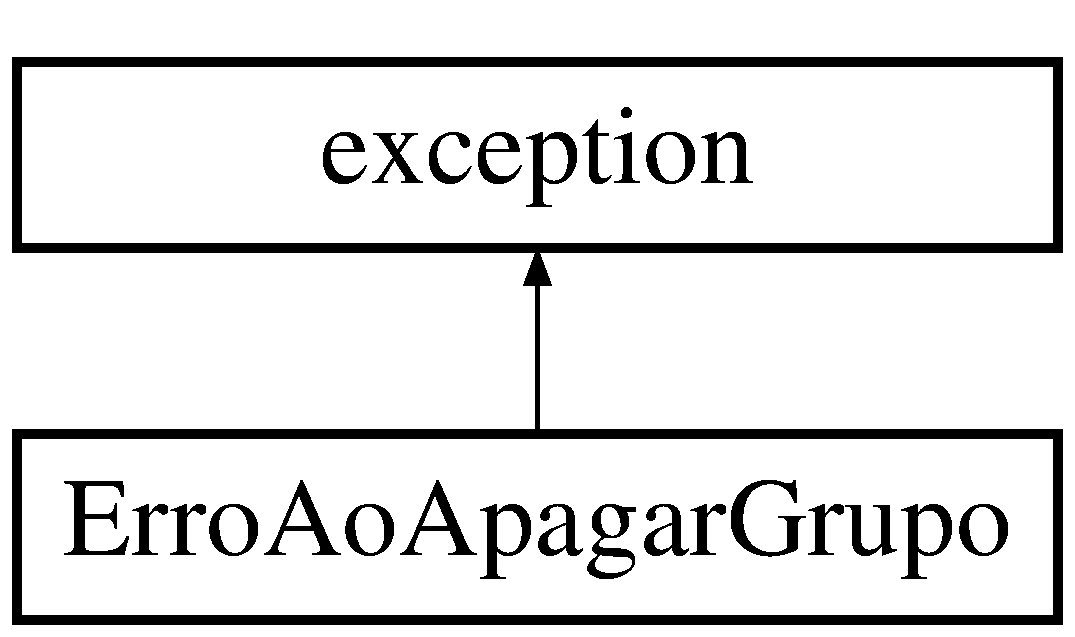
\includegraphics[height=2.000000cm]{classErroAoApagarGrupo}
\end{center}
\end{figure}
\subsection*{Public Member Functions}
\begin{DoxyCompactItemize}
\item 
const char $\ast$ \hyperlink{classErroAoApagarGrupo_a6857dcb5c67b480046e93e00d29c59ef}{what} () const noexcept override
\end{DoxyCompactItemize}
\subsection*{Private Attributes}
\begin{DoxyCompactItemize}
\item 
string \hyperlink{classErroAoApagarGrupo_a9a71b44cefcc19a8f9d4b8f97efa9ac5}{mensagem} = \char`\"{}Não é possivel apagar esse grupo pois existem tarefas associadas a ele.\char`\"{}
\end{DoxyCompactItemize}


\subsection{Member Function Documentation}
\mbox{\Hypertarget{classErroAoApagarGrupo_a6857dcb5c67b480046e93e00d29c59ef}\label{classErroAoApagarGrupo_a6857dcb5c67b480046e93e00d29c59ef}} 
\index{Erro\+Ao\+Apagar\+Grupo@{Erro\+Ao\+Apagar\+Grupo}!what@{what}}
\index{what@{what}!Erro\+Ao\+Apagar\+Grupo@{Erro\+Ao\+Apagar\+Grupo}}
\subsubsection{\texorpdfstring{what()}{what()}}
{\footnotesize\ttfamily const char$\ast$ Erro\+Ao\+Apagar\+Grupo\+::what (\begin{DoxyParamCaption}{ }\end{DoxyParamCaption}) const\hspace{0.3cm}{\ttfamily [inline]}, {\ttfamily [override]}, {\ttfamily [noexcept]}}



\subsection{Member Data Documentation}
\mbox{\Hypertarget{classErroAoApagarGrupo_a9a71b44cefcc19a8f9d4b8f97efa9ac5}\label{classErroAoApagarGrupo_a9a71b44cefcc19a8f9d4b8f97efa9ac5}} 
\index{Erro\+Ao\+Apagar\+Grupo@{Erro\+Ao\+Apagar\+Grupo}!mensagem@{mensagem}}
\index{mensagem@{mensagem}!Erro\+Ao\+Apagar\+Grupo@{Erro\+Ao\+Apagar\+Grupo}}
\subsubsection{\texorpdfstring{mensagem}{mensagem}}
{\footnotesize\ttfamily string Erro\+Ao\+Apagar\+Grupo\+::mensagem = \char`\"{}Não é possivel apagar esse grupo pois existem tarefas associadas a ele.\char`\"{}\hspace{0.3cm}{\ttfamily [private]}}



The documentation for this class was generated from the following file\+:\begin{DoxyCompactItemize}
\item 
include/excecoes/\hyperlink{exc__grupo_8hpp}{exc\+\_\+grupo.\+hpp}\end{DoxyCompactItemize}

\hypertarget{classErroAoApagarPrioridade}{}\section{Erro\+Ao\+Apagar\+Prioridade Class Reference}
\label{classErroAoApagarPrioridade}\index{Erro\+Ao\+Apagar\+Prioridade@{Erro\+Ao\+Apagar\+Prioridade}}


{\ttfamily \#include $<$exc\+\_\+prioridade.\+hpp$>$}

Inheritance diagram for Erro\+Ao\+Apagar\+Prioridade\+:\begin{figure}[H]
\begin{center}
\leavevmode
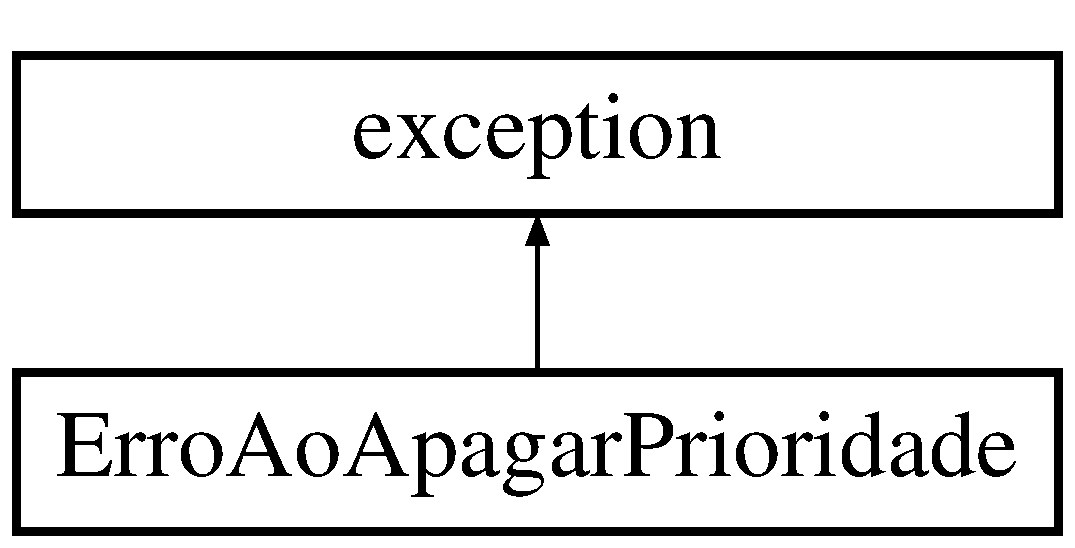
\includegraphics[height=2.000000cm]{classErroAoApagarPrioridade}
\end{center}
\end{figure}
\subsection*{Public Member Functions}
\begin{DoxyCompactItemize}
\item 
const char $\ast$ \hyperlink{classErroAoApagarPrioridade_ac6bc1bc5103de9f750fd5bda425db035}{what} () const noexcept override
\end{DoxyCompactItemize}
\subsection*{Private Attributes}
\begin{DoxyCompactItemize}
\item 
string \hyperlink{classErroAoApagarPrioridade_a97a77cb489c4dfea2fcd9084c31633e8}{mensagem} = \char`\"{}Não é possivel apagar essa prioridade pois existem tarefas associadas a ela.\char`\"{}
\end{DoxyCompactItemize}


\subsection{Member Function Documentation}
\mbox{\Hypertarget{classErroAoApagarPrioridade_ac6bc1bc5103de9f750fd5bda425db035}\label{classErroAoApagarPrioridade_ac6bc1bc5103de9f750fd5bda425db035}} 
\index{Erro\+Ao\+Apagar\+Prioridade@{Erro\+Ao\+Apagar\+Prioridade}!what@{what}}
\index{what@{what}!Erro\+Ao\+Apagar\+Prioridade@{Erro\+Ao\+Apagar\+Prioridade}}
\subsubsection{\texorpdfstring{what()}{what()}}
{\footnotesize\ttfamily const char$\ast$ Erro\+Ao\+Apagar\+Prioridade\+::what (\begin{DoxyParamCaption}{ }\end{DoxyParamCaption}) const\hspace{0.3cm}{\ttfamily [inline]}, {\ttfamily [override]}, {\ttfamily [noexcept]}}



\subsection{Member Data Documentation}
\mbox{\Hypertarget{classErroAoApagarPrioridade_a97a77cb489c4dfea2fcd9084c31633e8}\label{classErroAoApagarPrioridade_a97a77cb489c4dfea2fcd9084c31633e8}} 
\index{Erro\+Ao\+Apagar\+Prioridade@{Erro\+Ao\+Apagar\+Prioridade}!mensagem@{mensagem}}
\index{mensagem@{mensagem}!Erro\+Ao\+Apagar\+Prioridade@{Erro\+Ao\+Apagar\+Prioridade}}
\subsubsection{\texorpdfstring{mensagem}{mensagem}}
{\footnotesize\ttfamily string Erro\+Ao\+Apagar\+Prioridade\+::mensagem = \char`\"{}Não é possivel apagar essa prioridade pois existem tarefas associadas a ela.\char`\"{}\hspace{0.3cm}{\ttfamily [private]}}



The documentation for this class was generated from the following file\+:\begin{DoxyCompactItemize}
\item 
include/excecoes/\hyperlink{exc__prioridade_8hpp}{exc\+\_\+prioridade.\+hpp}\end{DoxyCompactItemize}

\hypertarget{classEtiqueta}{}\section{Etiqueta Class Reference}
\label{classEtiqueta}\index{Etiqueta@{Etiqueta}}


{\ttfamily \#include $<$etiqueta.\+hpp$>$}

Inheritance diagram for Etiqueta\+:\begin{figure}[H]
\begin{center}
\leavevmode
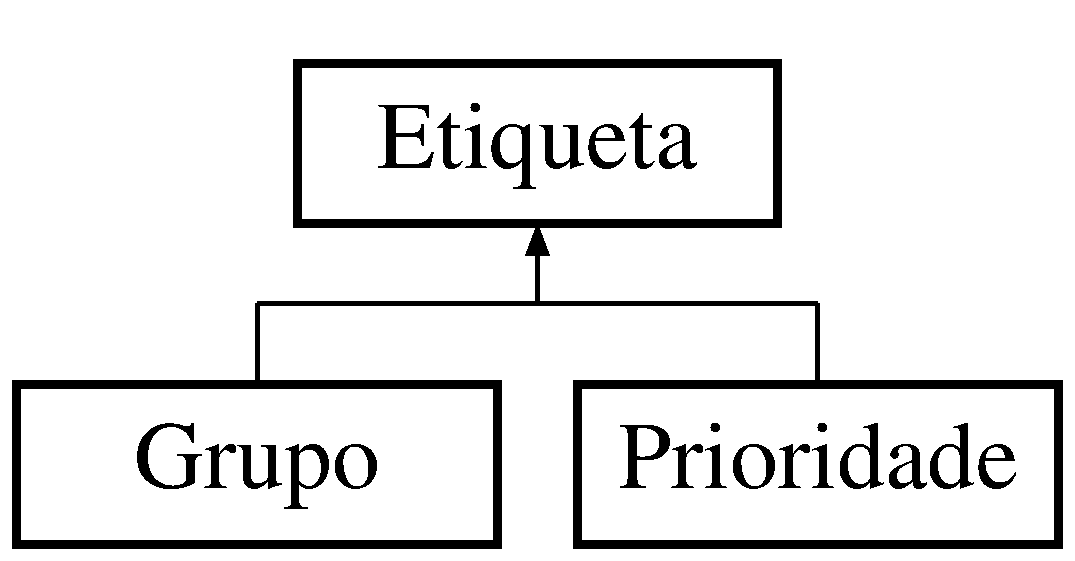
\includegraphics[height=2.000000cm]{classEtiqueta}
\end{center}
\end{figure}
\subsection*{Public Member Functions}
\begin{DoxyCompactItemize}
\item 
\hyperlink{classEtiqueta_aef0684cb6dc41c4f6f602b184ec64bce}{Etiqueta} (string nome\+\_\+etiqueta, string tipo)
\item 
string \hyperlink{classEtiqueta_a19d4e9c998e6b7fab0dafc88e9c7b9e2}{get\+\_\+nome\+\_\+etiqueta} ()
\item 
string \hyperlink{classEtiqueta_a27ea122e50442c29d7021fbe374ae4ea}{get\+\_\+tipo} ()
\item 
void \hyperlink{classEtiqueta_a1e19fda758d2d6118a3f9f8763bf50c2}{incrementa\+\_\+tarefa} ()
\item 
void \hyperlink{classEtiqueta_a01a51067b14191eba6f0fd7ac5d7a5bb}{decrementa\+\_\+tarefa} ()
\item 
int \hyperlink{classEtiqueta_a46c86502abf12a5824f1421a452fe239}{get\+\_\+qtd\+\_\+membros} ()
\end{DoxyCompactItemize}
\subsection*{Protected Attributes}
\begin{DoxyCompactItemize}
\item 
string \hyperlink{classEtiqueta_ad33c17ad4b54e7e8a1a760650747ee71}{\+\_\+nome\+\_\+etiqueta}
\item 
string \hyperlink{classEtiqueta_af4097d8bb6e190bb32c6bf70177f8b0c}{\+\_\+tipo}
\item 
int \hyperlink{classEtiqueta_af72d9ff60b84f4635e78f12ec8f80dab}{\+\_\+qtd\+\_\+membros}
\end{DoxyCompactItemize}


\subsection{Constructor \& Destructor Documentation}
\mbox{\Hypertarget{classEtiqueta_aef0684cb6dc41c4f6f602b184ec64bce}\label{classEtiqueta_aef0684cb6dc41c4f6f602b184ec64bce}} 
\index{Etiqueta@{Etiqueta}!Etiqueta@{Etiqueta}}
\index{Etiqueta@{Etiqueta}!Etiqueta@{Etiqueta}}
\subsubsection{\texorpdfstring{Etiqueta()}{Etiqueta()}}
{\footnotesize\ttfamily Etiqueta\+::\+Etiqueta (\begin{DoxyParamCaption}\item[{string}]{nome\+\_\+etiqueta,  }\item[{string}]{tipo }\end{DoxyParamCaption})}



\subsection{Member Function Documentation}
\mbox{\Hypertarget{classEtiqueta_a01a51067b14191eba6f0fd7ac5d7a5bb}\label{classEtiqueta_a01a51067b14191eba6f0fd7ac5d7a5bb}} 
\index{Etiqueta@{Etiqueta}!decrementa\+\_\+tarefa@{decrementa\+\_\+tarefa}}
\index{decrementa\+\_\+tarefa@{decrementa\+\_\+tarefa}!Etiqueta@{Etiqueta}}
\subsubsection{\texorpdfstring{decrementa\+\_\+tarefa()}{decrementa\_tarefa()}}
{\footnotesize\ttfamily void Etiqueta\+::decrementa\+\_\+tarefa (\begin{DoxyParamCaption}{ }\end{DoxyParamCaption})}

\mbox{\Hypertarget{classEtiqueta_a19d4e9c998e6b7fab0dafc88e9c7b9e2}\label{classEtiqueta_a19d4e9c998e6b7fab0dafc88e9c7b9e2}} 
\index{Etiqueta@{Etiqueta}!get\+\_\+nome\+\_\+etiqueta@{get\+\_\+nome\+\_\+etiqueta}}
\index{get\+\_\+nome\+\_\+etiqueta@{get\+\_\+nome\+\_\+etiqueta}!Etiqueta@{Etiqueta}}
\subsubsection{\texorpdfstring{get\+\_\+nome\+\_\+etiqueta()}{get\_nome\_etiqueta()}}
{\footnotesize\ttfamily string Etiqueta\+::get\+\_\+nome\+\_\+etiqueta (\begin{DoxyParamCaption}{ }\end{DoxyParamCaption})}

\mbox{\Hypertarget{classEtiqueta_a46c86502abf12a5824f1421a452fe239}\label{classEtiqueta_a46c86502abf12a5824f1421a452fe239}} 
\index{Etiqueta@{Etiqueta}!get\+\_\+qtd\+\_\+membros@{get\+\_\+qtd\+\_\+membros}}
\index{get\+\_\+qtd\+\_\+membros@{get\+\_\+qtd\+\_\+membros}!Etiqueta@{Etiqueta}}
\subsubsection{\texorpdfstring{get\+\_\+qtd\+\_\+membros()}{get\_qtd\_membros()}}
{\footnotesize\ttfamily int Etiqueta\+::get\+\_\+qtd\+\_\+membros (\begin{DoxyParamCaption}{ }\end{DoxyParamCaption})}

\mbox{\Hypertarget{classEtiqueta_a27ea122e50442c29d7021fbe374ae4ea}\label{classEtiqueta_a27ea122e50442c29d7021fbe374ae4ea}} 
\index{Etiqueta@{Etiqueta}!get\+\_\+tipo@{get\+\_\+tipo}}
\index{get\+\_\+tipo@{get\+\_\+tipo}!Etiqueta@{Etiqueta}}
\subsubsection{\texorpdfstring{get\+\_\+tipo()}{get\_tipo()}}
{\footnotesize\ttfamily string Etiqueta\+::get\+\_\+tipo (\begin{DoxyParamCaption}{ }\end{DoxyParamCaption})}

\mbox{\Hypertarget{classEtiqueta_a1e19fda758d2d6118a3f9f8763bf50c2}\label{classEtiqueta_a1e19fda758d2d6118a3f9f8763bf50c2}} 
\index{Etiqueta@{Etiqueta}!incrementa\+\_\+tarefa@{incrementa\+\_\+tarefa}}
\index{incrementa\+\_\+tarefa@{incrementa\+\_\+tarefa}!Etiqueta@{Etiqueta}}
\subsubsection{\texorpdfstring{incrementa\+\_\+tarefa()}{incrementa\_tarefa()}}
{\footnotesize\ttfamily void Etiqueta\+::incrementa\+\_\+tarefa (\begin{DoxyParamCaption}{ }\end{DoxyParamCaption})}



\subsection{Member Data Documentation}
\mbox{\Hypertarget{classEtiqueta_ad33c17ad4b54e7e8a1a760650747ee71}\label{classEtiqueta_ad33c17ad4b54e7e8a1a760650747ee71}} 
\index{Etiqueta@{Etiqueta}!\+\_\+nome\+\_\+etiqueta@{\+\_\+nome\+\_\+etiqueta}}
\index{\+\_\+nome\+\_\+etiqueta@{\+\_\+nome\+\_\+etiqueta}!Etiqueta@{Etiqueta}}
\subsubsection{\texorpdfstring{\+\_\+nome\+\_\+etiqueta}{\_nome\_etiqueta}}
{\footnotesize\ttfamily string Etiqueta\+::\+\_\+nome\+\_\+etiqueta\hspace{0.3cm}{\ttfamily [protected]}}

\mbox{\Hypertarget{classEtiqueta_af72d9ff60b84f4635e78f12ec8f80dab}\label{classEtiqueta_af72d9ff60b84f4635e78f12ec8f80dab}} 
\index{Etiqueta@{Etiqueta}!\+\_\+qtd\+\_\+membros@{\+\_\+qtd\+\_\+membros}}
\index{\+\_\+qtd\+\_\+membros@{\+\_\+qtd\+\_\+membros}!Etiqueta@{Etiqueta}}
\subsubsection{\texorpdfstring{\+\_\+qtd\+\_\+membros}{\_qtd\_membros}}
{\footnotesize\ttfamily int Etiqueta\+::\+\_\+qtd\+\_\+membros\hspace{0.3cm}{\ttfamily [protected]}}

\mbox{\Hypertarget{classEtiqueta_af4097d8bb6e190bb32c6bf70177f8b0c}\label{classEtiqueta_af4097d8bb6e190bb32c6bf70177f8b0c}} 
\index{Etiqueta@{Etiqueta}!\+\_\+tipo@{\+\_\+tipo}}
\index{\+\_\+tipo@{\+\_\+tipo}!Etiqueta@{Etiqueta}}
\subsubsection{\texorpdfstring{\+\_\+tipo}{\_tipo}}
{\footnotesize\ttfamily string Etiqueta\+::\+\_\+tipo\hspace{0.3cm}{\ttfamily [protected]}}



The documentation for this class was generated from the following file\+:\begin{DoxyCompactItemize}
\item 
include/\hyperlink{etiqueta_8hpp}{etiqueta.\+hpp}\end{DoxyCompactItemize}

\hypertarget{classFileUtil}{}\section{File\+Util Class Reference}
\label{classFileUtil}\index{File\+Util@{File\+Util}}


{\ttfamily \#include $<$file\+\_\+util.\+hpp$>$}

\subsection*{Static Public Member Functions}
\begin{DoxyCompactItemize}
\item 
static bool \hyperlink{classFileUtil_af2aa664a3cee3c3d9a0c07d4312e6c2d}{folder\+\_\+exists} (string folder\+\_\+name)
\item 
static bool \hyperlink{classFileUtil_a3ee8a43a763142c166ea87e50bbde33d}{file\+\_\+exists} (string file\+\_\+name)
\end{DoxyCompactItemize}


\subsection{Member Function Documentation}
\mbox{\Hypertarget{classFileUtil_a3ee8a43a763142c166ea87e50bbde33d}\label{classFileUtil_a3ee8a43a763142c166ea87e50bbde33d}} 
\index{File\+Util@{File\+Util}!file\+\_\+exists@{file\+\_\+exists}}
\index{file\+\_\+exists@{file\+\_\+exists}!File\+Util@{File\+Util}}
\subsubsection{\texorpdfstring{file\+\_\+exists()}{file\_exists()}}
{\footnotesize\ttfamily static bool File\+Util\+::file\+\_\+exists (\begin{DoxyParamCaption}\item[{string}]{file\+\_\+name }\end{DoxyParamCaption})\hspace{0.3cm}{\ttfamily [static]}}

\mbox{\Hypertarget{classFileUtil_af2aa664a3cee3c3d9a0c07d4312e6c2d}\label{classFileUtil_af2aa664a3cee3c3d9a0c07d4312e6c2d}} 
\index{File\+Util@{File\+Util}!folder\+\_\+exists@{folder\+\_\+exists}}
\index{folder\+\_\+exists@{folder\+\_\+exists}!File\+Util@{File\+Util}}
\subsubsection{\texorpdfstring{folder\+\_\+exists()}{folder\_exists()}}
{\footnotesize\ttfamily static bool File\+Util\+::folder\+\_\+exists (\begin{DoxyParamCaption}\item[{string}]{folder\+\_\+name }\end{DoxyParamCaption})\hspace{0.3cm}{\ttfamily [static]}}



The documentation for this class was generated from the following file\+:\begin{DoxyCompactItemize}
\item 
include/\hyperlink{file__util_8hpp}{file\+\_\+util.\+hpp}\end{DoxyCompactItemize}

\hypertarget{classGrupo}{}\section{Grupo Class Reference}
\label{classGrupo}\index{Grupo@{Grupo}}


{\ttfamily \#include $<$grupo.\+hpp$>$}

Inheritance diagram for Grupo\+:\begin{figure}[H]
\begin{center}
\leavevmode
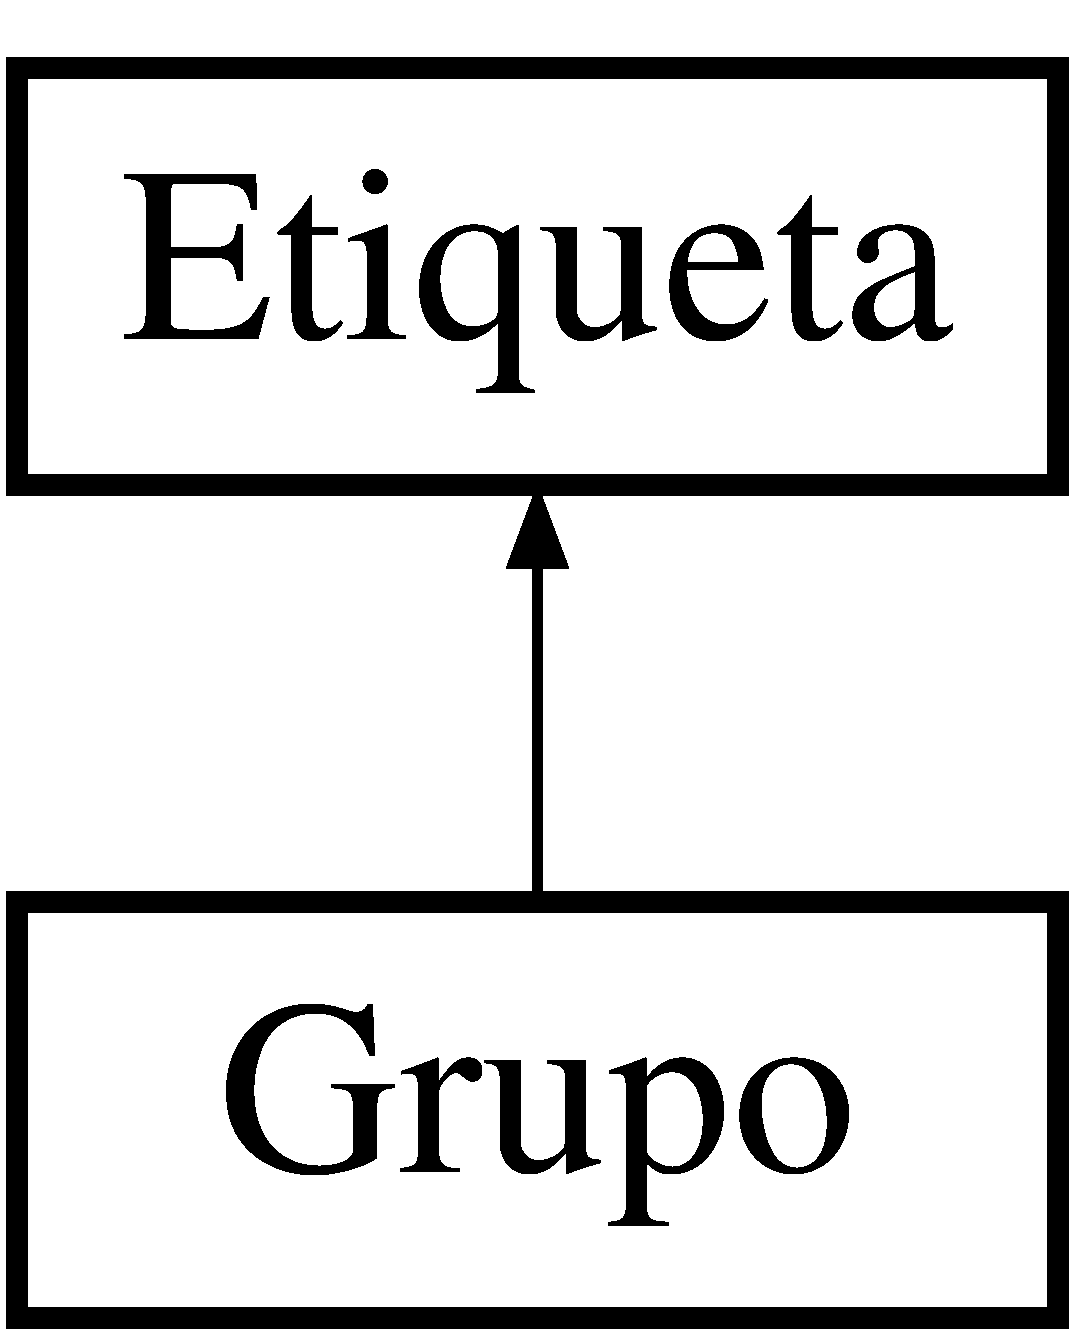
\includegraphics[height=2.000000cm]{classGrupo}
\end{center}
\end{figure}
\subsection*{Public Member Functions}
\begin{DoxyCompactItemize}
\item 
\hyperlink{classGrupo_a14745ea67ff25543b2cf949f765a726b}{Grupo} (string nome\+\_\+etiqueta, string tipo, string descricao)
\item 
int \hyperlink{classGrupo_a9d93d76de63fb7b7faca9e7c1d1c607a}{get\+\_\+qtd\+\_\+membros} ()
\item 
string \hyperlink{classGrupo_a750990ef2e00c1c56558aeacab25d5a9}{get\+\_\+descricao} ()
\item 
void \hyperlink{classGrupo_ad89de5bdcf8aa7913bb9d3cabe16aba1}{alterar} (string new\+\_\+grupo)
\item 
void \hyperlink{classGrupo_a307ca8081150b1c9784d22ff1d3d72d2}{alterar\+\_\+descricao} (string new\+\_\+descricao)
\end{DoxyCompactItemize}
\subsection*{Private Attributes}
\begin{DoxyCompactItemize}
\item 
string \hyperlink{classGrupo_a8f3c802c33537298ddbbc8b11bcea2f3}{\+\_\+descricao}
\end{DoxyCompactItemize}
\subsection*{Additional Inherited Members}


\subsection{Constructor \& Destructor Documentation}
\mbox{\Hypertarget{classGrupo_a14745ea67ff25543b2cf949f765a726b}\label{classGrupo_a14745ea67ff25543b2cf949f765a726b}} 
\index{Grupo@{Grupo}!Grupo@{Grupo}}
\index{Grupo@{Grupo}!Grupo@{Grupo}}
\subsubsection{\texorpdfstring{Grupo()}{Grupo()}}
{\footnotesize\ttfamily Grupo\+::\+Grupo (\begin{DoxyParamCaption}\item[{string}]{nome\+\_\+etiqueta,  }\item[{string}]{tipo,  }\item[{string}]{descricao }\end{DoxyParamCaption})}



\subsection{Member Function Documentation}
\mbox{\Hypertarget{classGrupo_ad89de5bdcf8aa7913bb9d3cabe16aba1}\label{classGrupo_ad89de5bdcf8aa7913bb9d3cabe16aba1}} 
\index{Grupo@{Grupo}!alterar@{alterar}}
\index{alterar@{alterar}!Grupo@{Grupo}}
\subsubsection{\texorpdfstring{alterar()}{alterar()}}
{\footnotesize\ttfamily void Grupo\+::alterar (\begin{DoxyParamCaption}\item[{string}]{new\+\_\+grupo }\end{DoxyParamCaption})}

\mbox{\Hypertarget{classGrupo_a307ca8081150b1c9784d22ff1d3d72d2}\label{classGrupo_a307ca8081150b1c9784d22ff1d3d72d2}} 
\index{Grupo@{Grupo}!alterar\+\_\+descricao@{alterar\+\_\+descricao}}
\index{alterar\+\_\+descricao@{alterar\+\_\+descricao}!Grupo@{Grupo}}
\subsubsection{\texorpdfstring{alterar\+\_\+descricao()}{alterar\_descricao()}}
{\footnotesize\ttfamily void Grupo\+::alterar\+\_\+descricao (\begin{DoxyParamCaption}\item[{string}]{new\+\_\+descricao }\end{DoxyParamCaption})}

\mbox{\Hypertarget{classGrupo_a750990ef2e00c1c56558aeacab25d5a9}\label{classGrupo_a750990ef2e00c1c56558aeacab25d5a9}} 
\index{Grupo@{Grupo}!get\+\_\+descricao@{get\+\_\+descricao}}
\index{get\+\_\+descricao@{get\+\_\+descricao}!Grupo@{Grupo}}
\subsubsection{\texorpdfstring{get\+\_\+descricao()}{get\_descricao()}}
{\footnotesize\ttfamily string Grupo\+::get\+\_\+descricao (\begin{DoxyParamCaption}{ }\end{DoxyParamCaption})}

\mbox{\Hypertarget{classGrupo_a9d93d76de63fb7b7faca9e7c1d1c607a}\label{classGrupo_a9d93d76de63fb7b7faca9e7c1d1c607a}} 
\index{Grupo@{Grupo}!get\+\_\+qtd\+\_\+membros@{get\+\_\+qtd\+\_\+membros}}
\index{get\+\_\+qtd\+\_\+membros@{get\+\_\+qtd\+\_\+membros}!Grupo@{Grupo}}
\subsubsection{\texorpdfstring{get\+\_\+qtd\+\_\+membros()}{get\_qtd\_membros()}}
{\footnotesize\ttfamily int Grupo\+::get\+\_\+qtd\+\_\+membros (\begin{DoxyParamCaption}{ }\end{DoxyParamCaption})}



\subsection{Member Data Documentation}
\mbox{\Hypertarget{classGrupo_a8f3c802c33537298ddbbc8b11bcea2f3}\label{classGrupo_a8f3c802c33537298ddbbc8b11bcea2f3}} 
\index{Grupo@{Grupo}!\+\_\+descricao@{\+\_\+descricao}}
\index{\+\_\+descricao@{\+\_\+descricao}!Grupo@{Grupo}}
\subsubsection{\texorpdfstring{\+\_\+descricao}{\_descricao}}
{\footnotesize\ttfamily string Grupo\+::\+\_\+descricao\hspace{0.3cm}{\ttfamily [private]}}



The documentation for this class was generated from the following file\+:\begin{DoxyCompactItemize}
\item 
include/\hyperlink{grupo_8hpp}{grupo.\+hpp}\end{DoxyCompactItemize}

\hypertarget{classGrupoJaExiste}{}\section{Grupo\+Ja\+Existe Class Reference}
\label{classGrupoJaExiste}\index{Grupo\+Ja\+Existe@{Grupo\+Ja\+Existe}}


{\ttfamily \#include $<$exc\+\_\+grupo.\+hpp$>$}

Inheritance diagram for Grupo\+Ja\+Existe\+:\begin{figure}[H]
\begin{center}
\leavevmode
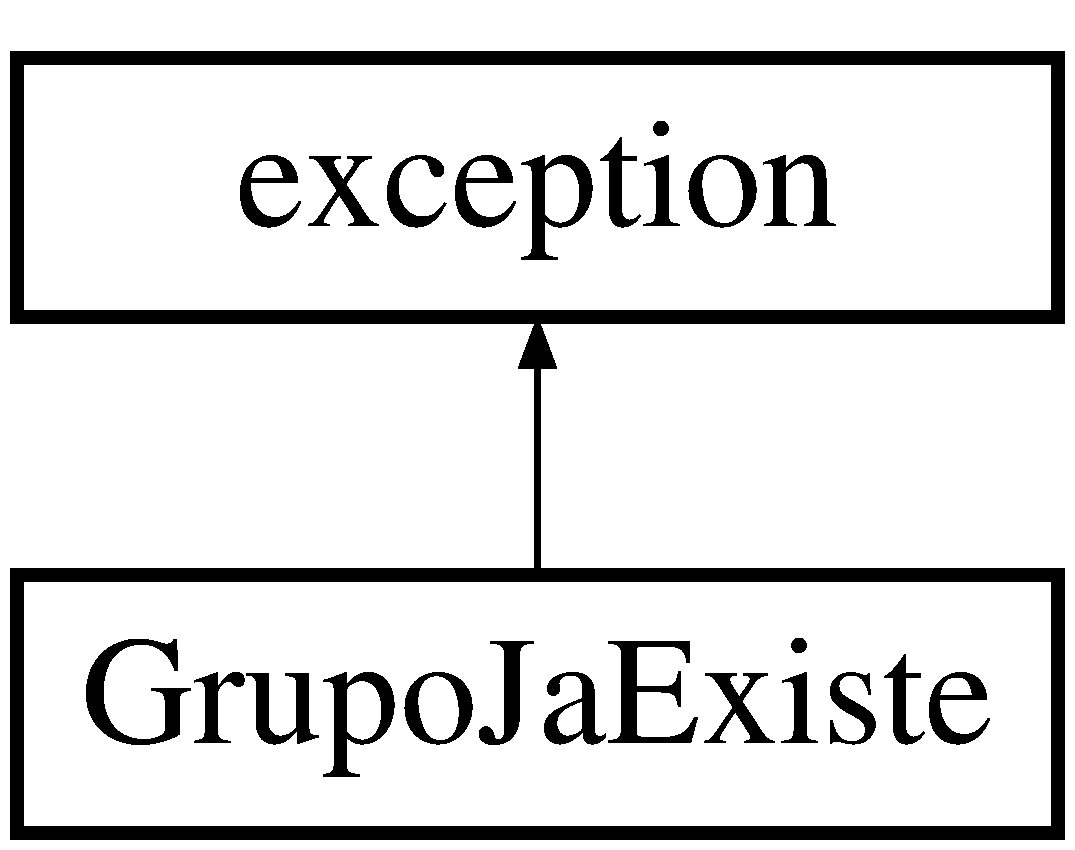
\includegraphics[height=2.000000cm]{classGrupoJaExiste}
\end{center}
\end{figure}
\subsection*{Public Member Functions}
\begin{DoxyCompactItemize}
\item 
const char $\ast$ \hyperlink{classGrupoJaExiste_a3a976953ceee43dbcadbf7638209b2c4}{what} () const noexcept override
\end{DoxyCompactItemize}
\subsection*{Private Attributes}
\begin{DoxyCompactItemize}
\item 
string \hyperlink{classGrupoJaExiste_aa2438c23067a525e7e1cdbf773b01dba}{mensagem} = \char`\"{}Já existe um grupo com esse nome. Tente novamente\char`\"{}
\end{DoxyCompactItemize}


\subsection{Member Function Documentation}
\mbox{\Hypertarget{classGrupoJaExiste_a3a976953ceee43dbcadbf7638209b2c4}\label{classGrupoJaExiste_a3a976953ceee43dbcadbf7638209b2c4}} 
\index{Grupo\+Ja\+Existe@{Grupo\+Ja\+Existe}!what@{what}}
\index{what@{what}!Grupo\+Ja\+Existe@{Grupo\+Ja\+Existe}}
\subsubsection{\texorpdfstring{what()}{what()}}
{\footnotesize\ttfamily const char$\ast$ Grupo\+Ja\+Existe\+::what (\begin{DoxyParamCaption}{ }\end{DoxyParamCaption}) const\hspace{0.3cm}{\ttfamily [inline]}, {\ttfamily [override]}, {\ttfamily [noexcept]}}



\subsection{Member Data Documentation}
\mbox{\Hypertarget{classGrupoJaExiste_aa2438c23067a525e7e1cdbf773b01dba}\label{classGrupoJaExiste_aa2438c23067a525e7e1cdbf773b01dba}} 
\index{Grupo\+Ja\+Existe@{Grupo\+Ja\+Existe}!mensagem@{mensagem}}
\index{mensagem@{mensagem}!Grupo\+Ja\+Existe@{Grupo\+Ja\+Existe}}
\subsubsection{\texorpdfstring{mensagem}{mensagem}}
{\footnotesize\ttfamily string Grupo\+Ja\+Existe\+::mensagem = \char`\"{}Já existe um grupo com esse nome. Tente novamente\char`\"{}\hspace{0.3cm}{\ttfamily [private]}}



The documentation for this class was generated from the following file\+:\begin{DoxyCompactItemize}
\item 
include/excecoes/\hyperlink{exc__grupo_8hpp}{exc\+\_\+grupo.\+hpp}\end{DoxyCompactItemize}

\hypertarget{classGrupoNaoExiste}{}\section{Grupo\+Nao\+Existe Class Reference}
\label{classGrupoNaoExiste}\index{Grupo\+Nao\+Existe@{Grupo\+Nao\+Existe}}


{\ttfamily \#include $<$exc\+\_\+grupo.\+hpp$>$}

Inheritance diagram for Grupo\+Nao\+Existe\+:\begin{figure}[H]
\begin{center}
\leavevmode
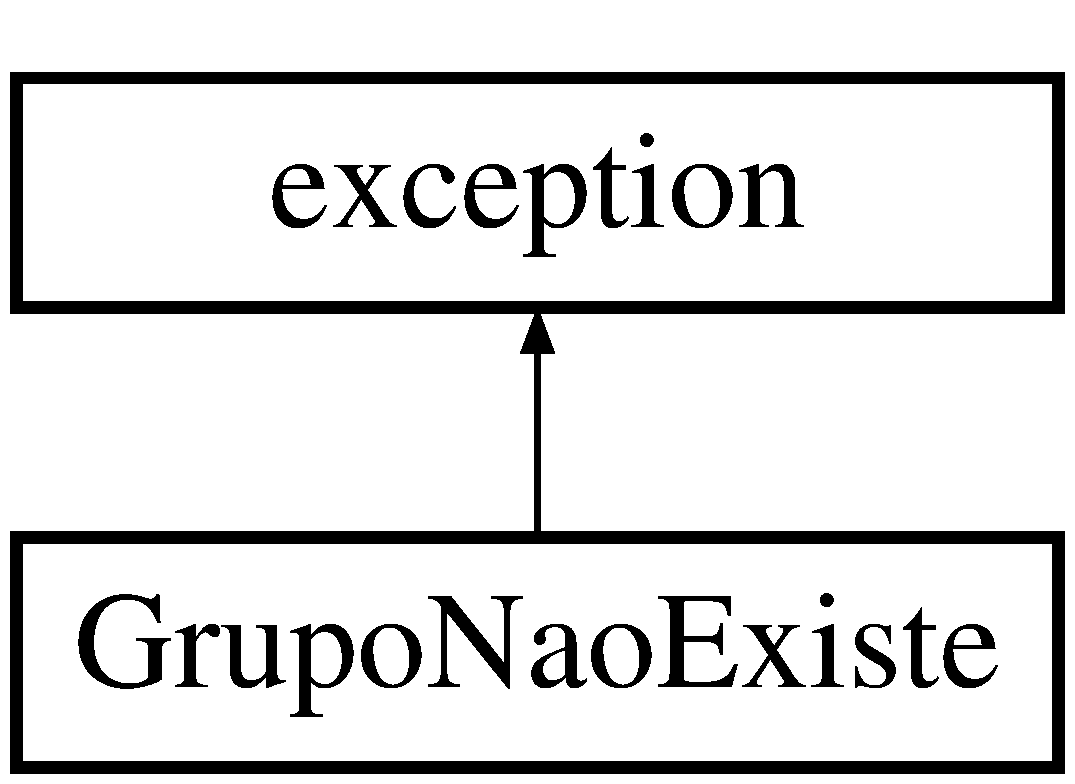
\includegraphics[height=2.000000cm]{classGrupoNaoExiste}
\end{center}
\end{figure}
\subsection*{Public Member Functions}
\begin{DoxyCompactItemize}
\item 
const char $\ast$ \hyperlink{classGrupoNaoExiste_afaddb4269a1b225b0f1045ae29fe8d6f}{what} () const noexcept override
\end{DoxyCompactItemize}
\subsection*{Private Attributes}
\begin{DoxyCompactItemize}
\item 
string \hyperlink{classGrupoNaoExiste_ae3a886240476581b33f88327c3282525}{mensagem} = \char`\"{}Não existe nenhum grupo com esse nome. Tente novamente\char`\"{}
\end{DoxyCompactItemize}


\subsection{Member Function Documentation}
\mbox{\Hypertarget{classGrupoNaoExiste_afaddb4269a1b225b0f1045ae29fe8d6f}\label{classGrupoNaoExiste_afaddb4269a1b225b0f1045ae29fe8d6f}} 
\index{Grupo\+Nao\+Existe@{Grupo\+Nao\+Existe}!what@{what}}
\index{what@{what}!Grupo\+Nao\+Existe@{Grupo\+Nao\+Existe}}
\subsubsection{\texorpdfstring{what()}{what()}}
{\footnotesize\ttfamily const char$\ast$ Grupo\+Nao\+Existe\+::what (\begin{DoxyParamCaption}{ }\end{DoxyParamCaption}) const\hspace{0.3cm}{\ttfamily [inline]}, {\ttfamily [override]}, {\ttfamily [noexcept]}}



\subsection{Member Data Documentation}
\mbox{\Hypertarget{classGrupoNaoExiste_ae3a886240476581b33f88327c3282525}\label{classGrupoNaoExiste_ae3a886240476581b33f88327c3282525}} 
\index{Grupo\+Nao\+Existe@{Grupo\+Nao\+Existe}!mensagem@{mensagem}}
\index{mensagem@{mensagem}!Grupo\+Nao\+Existe@{Grupo\+Nao\+Existe}}
\subsubsection{\texorpdfstring{mensagem}{mensagem}}
{\footnotesize\ttfamily string Grupo\+Nao\+Existe\+::mensagem = \char`\"{}Não existe nenhum grupo com esse nome. Tente novamente\char`\"{}\hspace{0.3cm}{\ttfamily [private]}}



The documentation for this class was generated from the following file\+:\begin{DoxyCompactItemize}
\item 
include/excecoes/\hyperlink{exc__grupo_8hpp}{exc\+\_\+grupo.\+hpp}\end{DoxyCompactItemize}

\hypertarget{classIdGrupoNaoExiste}{}\section{Id\+Grupo\+Nao\+Existe Class Reference}
\label{classIdGrupoNaoExiste}\index{Id\+Grupo\+Nao\+Existe@{Id\+Grupo\+Nao\+Existe}}


{\ttfamily \#include $<$exc\+\_\+grupo.\+hpp$>$}

Inheritance diagram for Id\+Grupo\+Nao\+Existe\+:\begin{figure}[H]
\begin{center}
\leavevmode
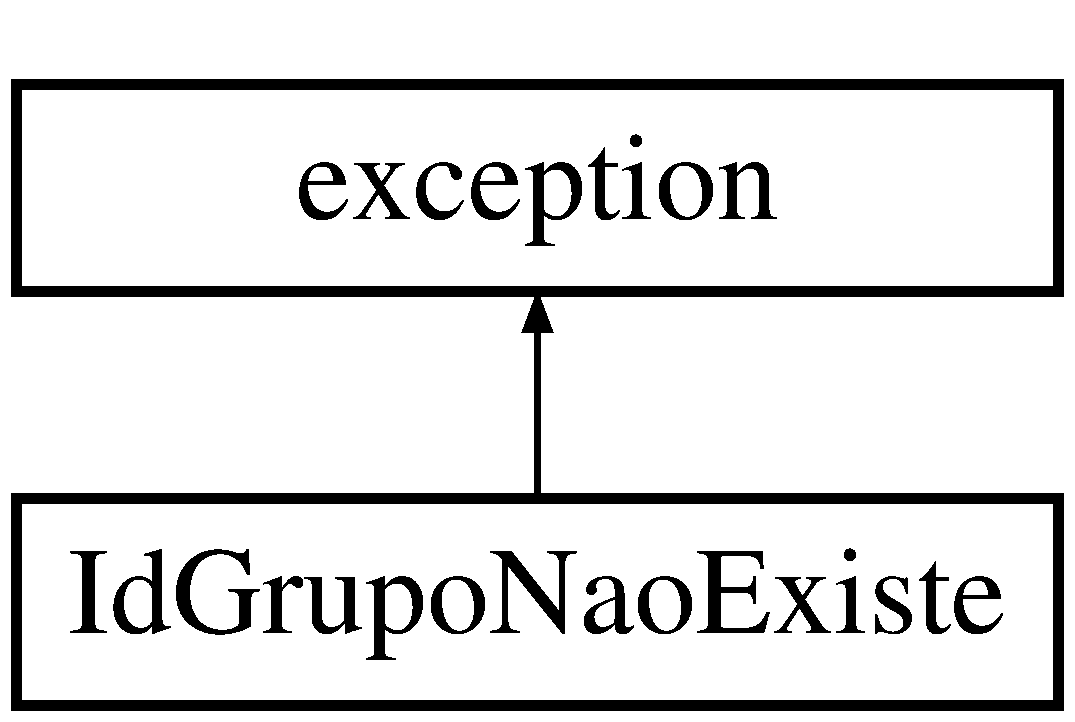
\includegraphics[height=2.000000cm]{classIdGrupoNaoExiste}
\end{center}
\end{figure}
\subsection*{Public Member Functions}
\begin{DoxyCompactItemize}
\item 
const char $\ast$ \hyperlink{classIdGrupoNaoExiste_a344839c288289dd67648514acb38da74}{what} () const noexcept override
\end{DoxyCompactItemize}
\subsection*{Private Attributes}
\begin{DoxyCompactItemize}
\item 
string \hyperlink{classIdGrupoNaoExiste_a75e9a2c40fb07070424acc3666b0babc}{mensagem} = \char`\"{}Não existe nenhum grupo com esse I\+D. Tente novamente\char`\"{}
\end{DoxyCompactItemize}


\subsection{Member Function Documentation}
\mbox{\Hypertarget{classIdGrupoNaoExiste_a344839c288289dd67648514acb38da74}\label{classIdGrupoNaoExiste_a344839c288289dd67648514acb38da74}} 
\index{Id\+Grupo\+Nao\+Existe@{Id\+Grupo\+Nao\+Existe}!what@{what}}
\index{what@{what}!Id\+Grupo\+Nao\+Existe@{Id\+Grupo\+Nao\+Existe}}
\subsubsection{\texorpdfstring{what()}{what()}}
{\footnotesize\ttfamily const char$\ast$ Id\+Grupo\+Nao\+Existe\+::what (\begin{DoxyParamCaption}{ }\end{DoxyParamCaption}) const\hspace{0.3cm}{\ttfamily [inline]}, {\ttfamily [override]}, {\ttfamily [noexcept]}}



\subsection{Member Data Documentation}
\mbox{\Hypertarget{classIdGrupoNaoExiste_a75e9a2c40fb07070424acc3666b0babc}\label{classIdGrupoNaoExiste_a75e9a2c40fb07070424acc3666b0babc}} 
\index{Id\+Grupo\+Nao\+Existe@{Id\+Grupo\+Nao\+Existe}!mensagem@{mensagem}}
\index{mensagem@{mensagem}!Id\+Grupo\+Nao\+Existe@{Id\+Grupo\+Nao\+Existe}}
\subsubsection{\texorpdfstring{mensagem}{mensagem}}
{\footnotesize\ttfamily string Id\+Grupo\+Nao\+Existe\+::mensagem = \char`\"{}Não existe nenhum grupo com esse I\+D. Tente novamente\char`\"{}\hspace{0.3cm}{\ttfamily [private]}}



The documentation for this class was generated from the following file\+:\begin{DoxyCompactItemize}
\item 
include/excecoes/\hyperlink{exc__grupo_8hpp}{exc\+\_\+grupo.\+hpp}\end{DoxyCompactItemize}

\hypertarget{classIdPrioridadeNaoExiste}{}\section{Id\+Prioridade\+Nao\+Existe Class Reference}
\label{classIdPrioridadeNaoExiste}\index{Id\+Prioridade\+Nao\+Existe@{Id\+Prioridade\+Nao\+Existe}}


{\ttfamily \#include $<$exc\+\_\+prioridade.\+hpp$>$}

Inheritance diagram for Id\+Prioridade\+Nao\+Existe\+:\begin{figure}[H]
\begin{center}
\leavevmode
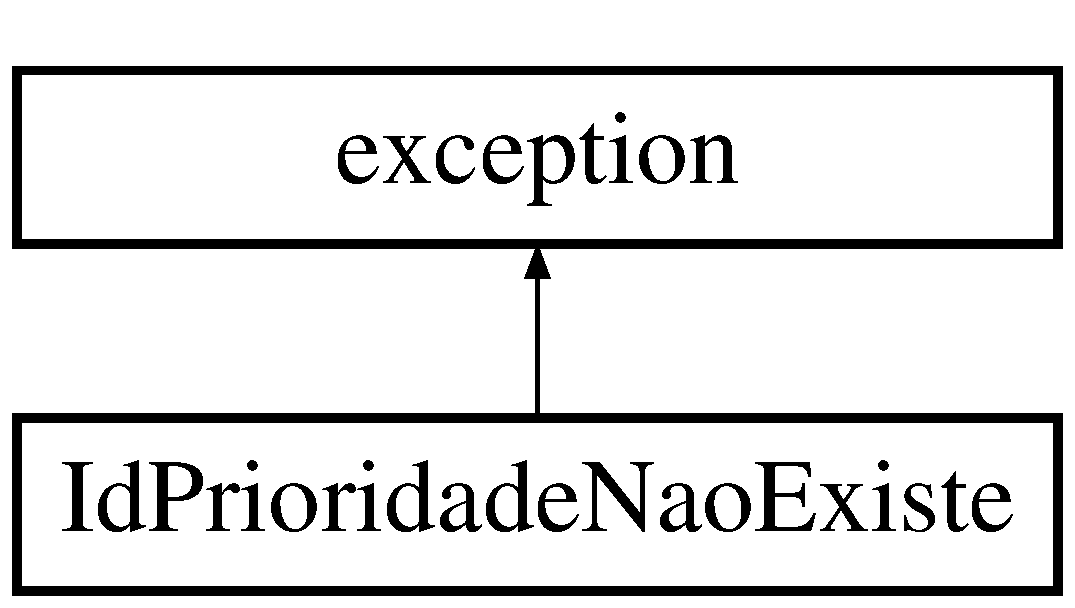
\includegraphics[height=2.000000cm]{classIdPrioridadeNaoExiste}
\end{center}
\end{figure}
\subsection*{Public Member Functions}
\begin{DoxyCompactItemize}
\item 
const char $\ast$ \hyperlink{classIdPrioridadeNaoExiste_a9e04482f29c7ed2c98fe3a388c6781d1}{what} () const noexcept override
\end{DoxyCompactItemize}
\subsection*{Private Attributes}
\begin{DoxyCompactItemize}
\item 
string \hyperlink{classIdPrioridadeNaoExiste_a0dc8383d0ca6ae78bf02a7429604bf63}{mensagem} = \char`\"{}Não existe nenhuma prioridade com esse I\+D. Tente novamente\char`\"{}
\end{DoxyCompactItemize}


\subsection{Member Function Documentation}
\mbox{\Hypertarget{classIdPrioridadeNaoExiste_a9e04482f29c7ed2c98fe3a388c6781d1}\label{classIdPrioridadeNaoExiste_a9e04482f29c7ed2c98fe3a388c6781d1}} 
\index{Id\+Prioridade\+Nao\+Existe@{Id\+Prioridade\+Nao\+Existe}!what@{what}}
\index{what@{what}!Id\+Prioridade\+Nao\+Existe@{Id\+Prioridade\+Nao\+Existe}}
\subsubsection{\texorpdfstring{what()}{what()}}
{\footnotesize\ttfamily const char$\ast$ Id\+Prioridade\+Nao\+Existe\+::what (\begin{DoxyParamCaption}{ }\end{DoxyParamCaption}) const\hspace{0.3cm}{\ttfamily [inline]}, {\ttfamily [override]}, {\ttfamily [noexcept]}}



\subsection{Member Data Documentation}
\mbox{\Hypertarget{classIdPrioridadeNaoExiste_a0dc8383d0ca6ae78bf02a7429604bf63}\label{classIdPrioridadeNaoExiste_a0dc8383d0ca6ae78bf02a7429604bf63}} 
\index{Id\+Prioridade\+Nao\+Existe@{Id\+Prioridade\+Nao\+Existe}!mensagem@{mensagem}}
\index{mensagem@{mensagem}!Id\+Prioridade\+Nao\+Existe@{Id\+Prioridade\+Nao\+Existe}}
\subsubsection{\texorpdfstring{mensagem}{mensagem}}
{\footnotesize\ttfamily string Id\+Prioridade\+Nao\+Existe\+::mensagem = \char`\"{}Não existe nenhuma prioridade com esse I\+D. Tente novamente\char`\"{}\hspace{0.3cm}{\ttfamily [private]}}



The documentation for this class was generated from the following file\+:\begin{DoxyCompactItemize}
\item 
include/excecoes/\hyperlink{exc__prioridade_8hpp}{exc\+\_\+prioridade.\+hpp}\end{DoxyCompactItemize}

\hypertarget{classIdTarefaNaoExiste}{}\section{Id\+Tarefa\+Nao\+Existe Class Reference}
\label{classIdTarefaNaoExiste}\index{Id\+Tarefa\+Nao\+Existe@{Id\+Tarefa\+Nao\+Existe}}


{\ttfamily \#include $<$exc\+\_\+tarefa.\+hpp$>$}

Inheritance diagram for Id\+Tarefa\+Nao\+Existe\+:\begin{figure}[H]
\begin{center}
\leavevmode
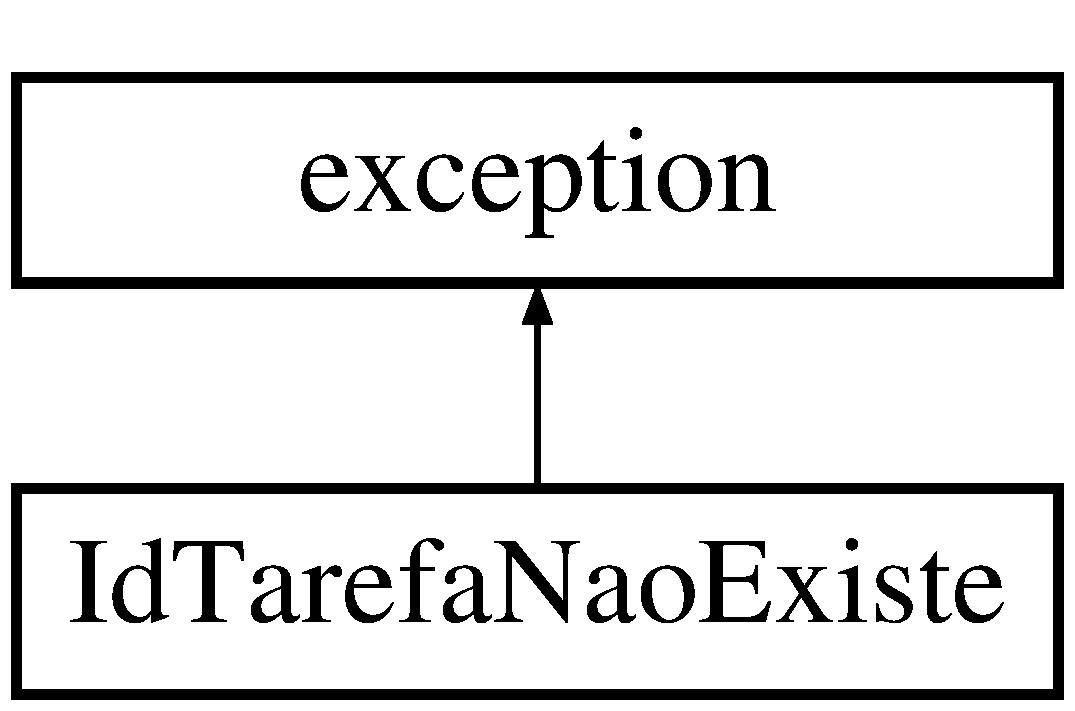
\includegraphics[height=2.000000cm]{classIdTarefaNaoExiste}
\end{center}
\end{figure}
\subsection*{Public Member Functions}
\begin{DoxyCompactItemize}
\item 
const char $\ast$ \hyperlink{classIdTarefaNaoExiste_a0e69982b6d345fe04e5a18c60d1e10f6}{what} () const noexcept override
\end{DoxyCompactItemize}
\subsection*{Private Attributes}
\begin{DoxyCompactItemize}
\item 
string \hyperlink{classIdTarefaNaoExiste_a139ea7adf62da317199adb6c77fb95bf}{mensagem} = \char`\"{}Não existe nenhuma tarefa com esse I\+D. Tente novamente\char`\"{}
\end{DoxyCompactItemize}


\subsection{Member Function Documentation}
\mbox{\Hypertarget{classIdTarefaNaoExiste_a0e69982b6d345fe04e5a18c60d1e10f6}\label{classIdTarefaNaoExiste_a0e69982b6d345fe04e5a18c60d1e10f6}} 
\index{Id\+Tarefa\+Nao\+Existe@{Id\+Tarefa\+Nao\+Existe}!what@{what}}
\index{what@{what}!Id\+Tarefa\+Nao\+Existe@{Id\+Tarefa\+Nao\+Existe}}
\subsubsection{\texorpdfstring{what()}{what()}}
{\footnotesize\ttfamily const char$\ast$ Id\+Tarefa\+Nao\+Existe\+::what (\begin{DoxyParamCaption}{ }\end{DoxyParamCaption}) const\hspace{0.3cm}{\ttfamily [inline]}, {\ttfamily [override]}, {\ttfamily [noexcept]}}



\subsection{Member Data Documentation}
\mbox{\Hypertarget{classIdTarefaNaoExiste_a139ea7adf62da317199adb6c77fb95bf}\label{classIdTarefaNaoExiste_a139ea7adf62da317199adb6c77fb95bf}} 
\index{Id\+Tarefa\+Nao\+Existe@{Id\+Tarefa\+Nao\+Existe}!mensagem@{mensagem}}
\index{mensagem@{mensagem}!Id\+Tarefa\+Nao\+Existe@{Id\+Tarefa\+Nao\+Existe}}
\subsubsection{\texorpdfstring{mensagem}{mensagem}}
{\footnotesize\ttfamily string Id\+Tarefa\+Nao\+Existe\+::mensagem = \char`\"{}Não existe nenhuma tarefa com esse I\+D. Tente novamente\char`\"{}\hspace{0.3cm}{\ttfamily [private]}}



The documentation for this class was generated from the following file\+:\begin{DoxyCompactItemize}
\item 
include/excecoes/\hyperlink{exc__tarefa_8hpp}{exc\+\_\+tarefa.\+hpp}\end{DoxyCompactItemize}

\hypertarget{classNomeGrupoMuitoLongo}{}\section{Nome\+Grupo\+Muito\+Longo Class Reference}
\label{classNomeGrupoMuitoLongo}\index{Nome\+Grupo\+Muito\+Longo@{Nome\+Grupo\+Muito\+Longo}}


{\ttfamily \#include $<$exc\+\_\+grupo.\+hpp$>$}

Inheritance diagram for Nome\+Grupo\+Muito\+Longo\+:\begin{figure}[H]
\begin{center}
\leavevmode
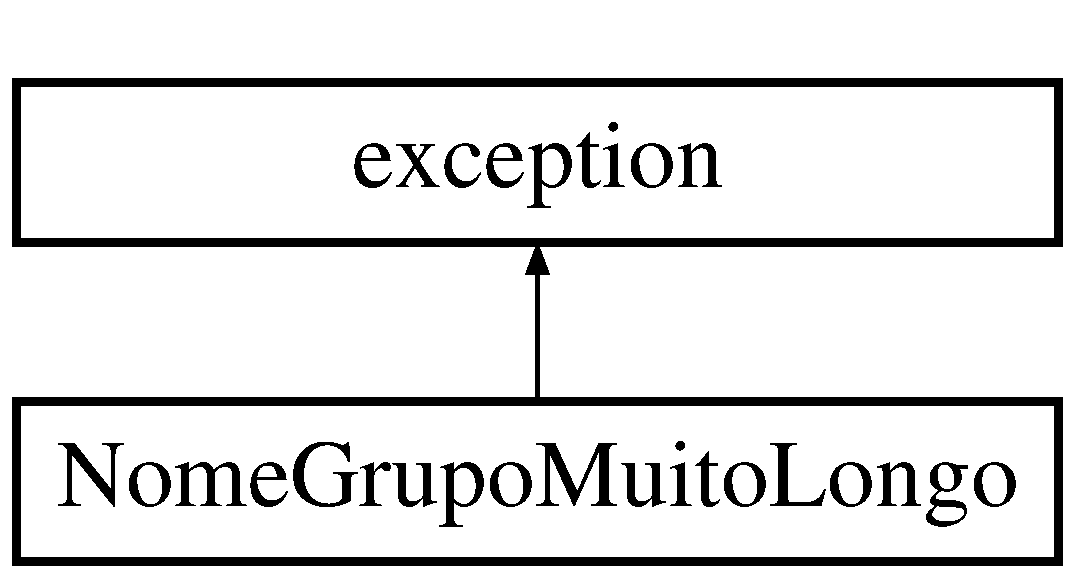
\includegraphics[height=2.000000cm]{classNomeGrupoMuitoLongo}
\end{center}
\end{figure}
\subsection*{Public Member Functions}
\begin{DoxyCompactItemize}
\item 
const char $\ast$ \hyperlink{classNomeGrupoMuitoLongo_a2b75f8838ba032215a34cba6cf9f52b7}{what} () const noexcept override
\end{DoxyCompactItemize}
\subsection*{Private Attributes}
\begin{DoxyCompactItemize}
\item 
string \hyperlink{classNomeGrupoMuitoLongo_a41c3c15095f9045cad1563e8f2257bbc}{mensagem} = \char`\"{}O nome do grupo não pode ter mais que 15 caracteres. Tente novamente\char`\"{}
\end{DoxyCompactItemize}


\subsection{Member Function Documentation}
\mbox{\Hypertarget{classNomeGrupoMuitoLongo_a2b75f8838ba032215a34cba6cf9f52b7}\label{classNomeGrupoMuitoLongo_a2b75f8838ba032215a34cba6cf9f52b7}} 
\index{Nome\+Grupo\+Muito\+Longo@{Nome\+Grupo\+Muito\+Longo}!what@{what}}
\index{what@{what}!Nome\+Grupo\+Muito\+Longo@{Nome\+Grupo\+Muito\+Longo}}
\subsubsection{\texorpdfstring{what()}{what()}}
{\footnotesize\ttfamily const char$\ast$ Nome\+Grupo\+Muito\+Longo\+::what (\begin{DoxyParamCaption}{ }\end{DoxyParamCaption}) const\hspace{0.3cm}{\ttfamily [inline]}, {\ttfamily [override]}, {\ttfamily [noexcept]}}



\subsection{Member Data Documentation}
\mbox{\Hypertarget{classNomeGrupoMuitoLongo_a41c3c15095f9045cad1563e8f2257bbc}\label{classNomeGrupoMuitoLongo_a41c3c15095f9045cad1563e8f2257bbc}} 
\index{Nome\+Grupo\+Muito\+Longo@{Nome\+Grupo\+Muito\+Longo}!mensagem@{mensagem}}
\index{mensagem@{mensagem}!Nome\+Grupo\+Muito\+Longo@{Nome\+Grupo\+Muito\+Longo}}
\subsubsection{\texorpdfstring{mensagem}{mensagem}}
{\footnotesize\ttfamily string Nome\+Grupo\+Muito\+Longo\+::mensagem = \char`\"{}O nome do grupo não pode ter mais que 15 caracteres. Tente novamente\char`\"{}\hspace{0.3cm}{\ttfamily [private]}}



The documentation for this class was generated from the following file\+:\begin{DoxyCompactItemize}
\item 
include/excecoes/\hyperlink{exc__grupo_8hpp}{exc\+\_\+grupo.\+hpp}\end{DoxyCompactItemize}

\hypertarget{classNomePrioridadeMuitoLongo}{}\section{Nome\+Prioridade\+Muito\+Longo Class Reference}
\label{classNomePrioridadeMuitoLongo}\index{Nome\+Prioridade\+Muito\+Longo@{Nome\+Prioridade\+Muito\+Longo}}


{\ttfamily \#include $<$exc\+\_\+prioridade.\+hpp$>$}

Inheritance diagram for Nome\+Prioridade\+Muito\+Longo\+:\begin{figure}[H]
\begin{center}
\leavevmode
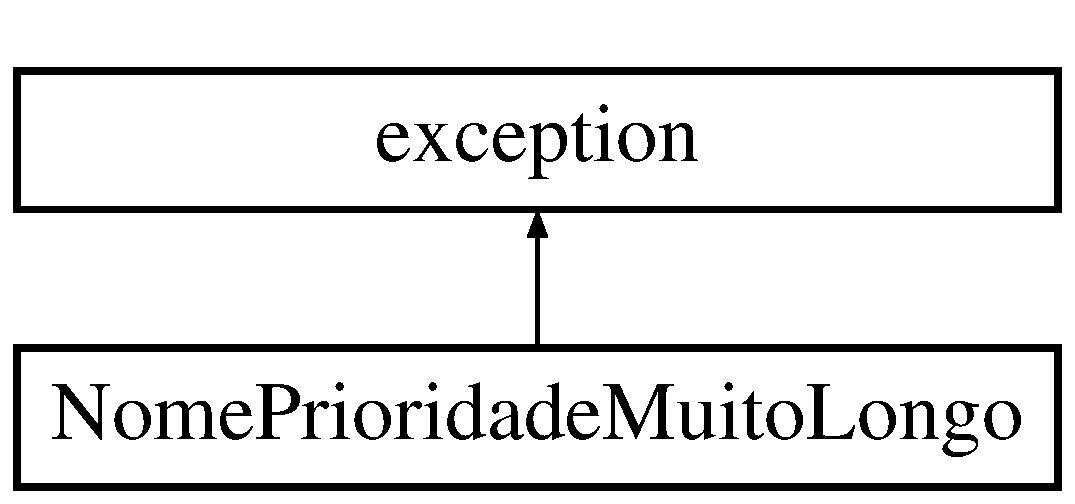
\includegraphics[height=2.000000cm]{classNomePrioridadeMuitoLongo}
\end{center}
\end{figure}
\subsection*{Public Member Functions}
\begin{DoxyCompactItemize}
\item 
const char $\ast$ \hyperlink{classNomePrioridadeMuitoLongo_a47faeee7100e964cb4bd8db518043316}{what} () const noexcept override
\end{DoxyCompactItemize}
\subsection*{Private Attributes}
\begin{DoxyCompactItemize}
\item 
string \hyperlink{classNomePrioridadeMuitoLongo_aa80f887bae3a735020c0113998991345}{mensagem} = \char`\"{}O nome da prioridade não pode ter mais que 15 caracteres. Tente novamente\char`\"{}
\end{DoxyCompactItemize}


\subsection{Member Function Documentation}
\mbox{\Hypertarget{classNomePrioridadeMuitoLongo_a47faeee7100e964cb4bd8db518043316}\label{classNomePrioridadeMuitoLongo_a47faeee7100e964cb4bd8db518043316}} 
\index{Nome\+Prioridade\+Muito\+Longo@{Nome\+Prioridade\+Muito\+Longo}!what@{what}}
\index{what@{what}!Nome\+Prioridade\+Muito\+Longo@{Nome\+Prioridade\+Muito\+Longo}}
\subsubsection{\texorpdfstring{what()}{what()}}
{\footnotesize\ttfamily const char$\ast$ Nome\+Prioridade\+Muito\+Longo\+::what (\begin{DoxyParamCaption}{ }\end{DoxyParamCaption}) const\hspace{0.3cm}{\ttfamily [inline]}, {\ttfamily [override]}, {\ttfamily [noexcept]}}



\subsection{Member Data Documentation}
\mbox{\Hypertarget{classNomePrioridadeMuitoLongo_aa80f887bae3a735020c0113998991345}\label{classNomePrioridadeMuitoLongo_aa80f887bae3a735020c0113998991345}} 
\index{Nome\+Prioridade\+Muito\+Longo@{Nome\+Prioridade\+Muito\+Longo}!mensagem@{mensagem}}
\index{mensagem@{mensagem}!Nome\+Prioridade\+Muito\+Longo@{Nome\+Prioridade\+Muito\+Longo}}
\subsubsection{\texorpdfstring{mensagem}{mensagem}}
{\footnotesize\ttfamily string Nome\+Prioridade\+Muito\+Longo\+::mensagem = \char`\"{}O nome da prioridade não pode ter mais que 15 caracteres. Tente novamente\char`\"{}\hspace{0.3cm}{\ttfamily [private]}}



The documentation for this class was generated from the following file\+:\begin{DoxyCompactItemize}
\item 
include/excecoes/\hyperlink{exc__prioridade_8hpp}{exc\+\_\+prioridade.\+hpp}\end{DoxyCompactItemize}

\hypertarget{classNomeTarefaMuitoLongo}{}\section{Nome\+Tarefa\+Muito\+Longo Class Reference}
\label{classNomeTarefaMuitoLongo}\index{Nome\+Tarefa\+Muito\+Longo@{Nome\+Tarefa\+Muito\+Longo}}


{\ttfamily \#include $<$exc\+\_\+tarefa.\+hpp$>$}

Inheritance diagram for Nome\+Tarefa\+Muito\+Longo\+:\begin{figure}[H]
\begin{center}
\leavevmode
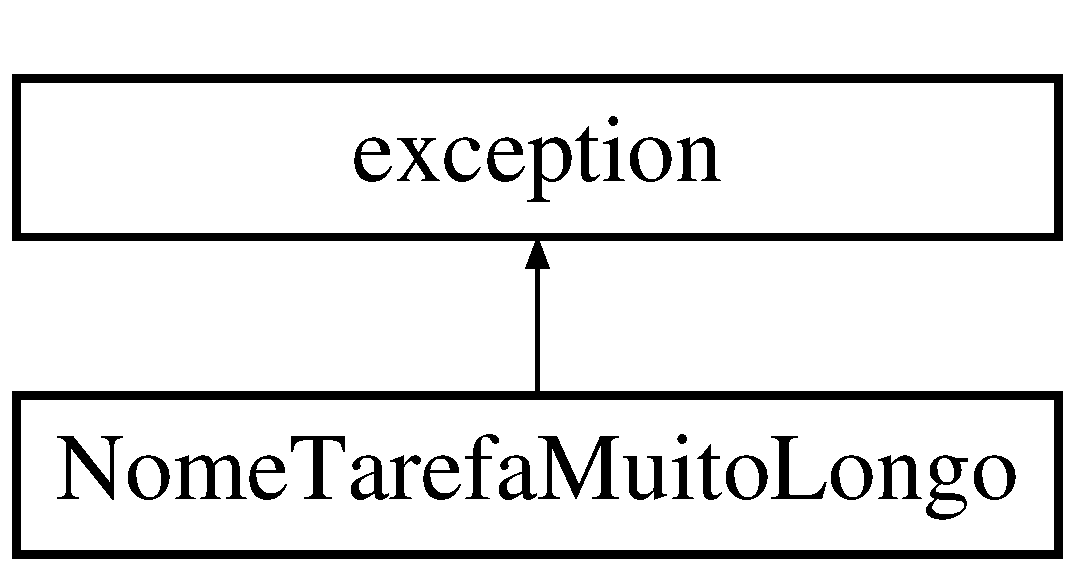
\includegraphics[height=2.000000cm]{classNomeTarefaMuitoLongo}
\end{center}
\end{figure}
\subsection*{Public Member Functions}
\begin{DoxyCompactItemize}
\item 
const char $\ast$ \hyperlink{classNomeTarefaMuitoLongo_af174669e16f0604829cd61d03809ed75}{what} () const noexcept override
\end{DoxyCompactItemize}
\subsection*{Private Attributes}
\begin{DoxyCompactItemize}
\item 
string \hyperlink{classNomeTarefaMuitoLongo_a72f730ba8580b5cd8efc1cee8f9ca4c9}{mensagem} = \char`\"{}O nome da tarefa não pode ter mais que 30 caracteres. Tente novamente\char`\"{}
\end{DoxyCompactItemize}


\subsection{Member Function Documentation}
\mbox{\Hypertarget{classNomeTarefaMuitoLongo_af174669e16f0604829cd61d03809ed75}\label{classNomeTarefaMuitoLongo_af174669e16f0604829cd61d03809ed75}} 
\index{Nome\+Tarefa\+Muito\+Longo@{Nome\+Tarefa\+Muito\+Longo}!what@{what}}
\index{what@{what}!Nome\+Tarefa\+Muito\+Longo@{Nome\+Tarefa\+Muito\+Longo}}
\subsubsection{\texorpdfstring{what()}{what()}}
{\footnotesize\ttfamily const char$\ast$ Nome\+Tarefa\+Muito\+Longo\+::what (\begin{DoxyParamCaption}{ }\end{DoxyParamCaption}) const\hspace{0.3cm}{\ttfamily [inline]}, {\ttfamily [override]}, {\ttfamily [noexcept]}}



\subsection{Member Data Documentation}
\mbox{\Hypertarget{classNomeTarefaMuitoLongo_a72f730ba8580b5cd8efc1cee8f9ca4c9}\label{classNomeTarefaMuitoLongo_a72f730ba8580b5cd8efc1cee8f9ca4c9}} 
\index{Nome\+Tarefa\+Muito\+Longo@{Nome\+Tarefa\+Muito\+Longo}!mensagem@{mensagem}}
\index{mensagem@{mensagem}!Nome\+Tarefa\+Muito\+Longo@{Nome\+Tarefa\+Muito\+Longo}}
\subsubsection{\texorpdfstring{mensagem}{mensagem}}
{\footnotesize\ttfamily string Nome\+Tarefa\+Muito\+Longo\+::mensagem = \char`\"{}O nome da tarefa não pode ter mais que 30 caracteres. Tente novamente\char`\"{}\hspace{0.3cm}{\ttfamily [private]}}



The documentation for this class was generated from the following file\+:\begin{DoxyCompactItemize}
\item 
include/excecoes/\hyperlink{exc__tarefa_8hpp}{exc\+\_\+tarefa.\+hpp}\end{DoxyCompactItemize}

\hypertarget{classPaginaInvalida}{}\section{Pagina\+Invalida Class Reference}
\label{classPaginaInvalida}\index{Pagina\+Invalida@{Pagina\+Invalida}}


{\ttfamily \#include $<$exc\+\_\+pagina.\+hpp$>$}

Inheritance diagram for Pagina\+Invalida\+:\begin{figure}[H]
\begin{center}
\leavevmode
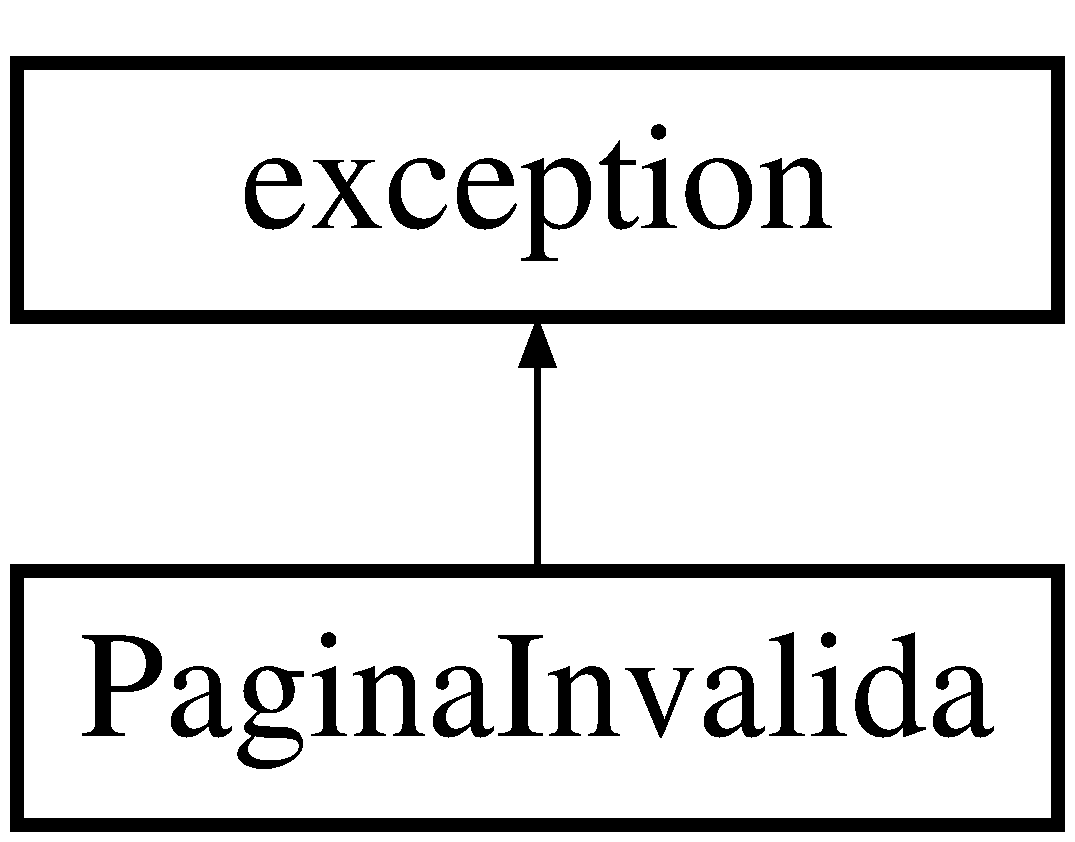
\includegraphics[height=2.000000cm]{classPaginaInvalida}
\end{center}
\end{figure}
\subsection*{Public Member Functions}
\begin{DoxyCompactItemize}
\item 
const char $\ast$ \hyperlink{classPaginaInvalida_a4022cf89811330d6505d8ed01cbc9132}{what} () const noexcept override
\end{DoxyCompactItemize}
\subsection*{Private Attributes}
\begin{DoxyCompactItemize}
\item 
string \hyperlink{classPaginaInvalida_aebeaffd6e9c09496a4a9d6ed2b87d0f9}{mensagem} = \char`\"{}Essa página não existe. Escolha uma página válida.\char`\"{}
\end{DoxyCompactItemize}


\subsection{Member Function Documentation}
\mbox{\Hypertarget{classPaginaInvalida_a4022cf89811330d6505d8ed01cbc9132}\label{classPaginaInvalida_a4022cf89811330d6505d8ed01cbc9132}} 
\index{Pagina\+Invalida@{Pagina\+Invalida}!what@{what}}
\index{what@{what}!Pagina\+Invalida@{Pagina\+Invalida}}
\subsubsection{\texorpdfstring{what()}{what()}}
{\footnotesize\ttfamily const char$\ast$ Pagina\+Invalida\+::what (\begin{DoxyParamCaption}{ }\end{DoxyParamCaption}) const\hspace{0.3cm}{\ttfamily [inline]}, {\ttfamily [override]}, {\ttfamily [noexcept]}}



\subsection{Member Data Documentation}
\mbox{\Hypertarget{classPaginaInvalida_aebeaffd6e9c09496a4a9d6ed2b87d0f9}\label{classPaginaInvalida_aebeaffd6e9c09496a4a9d6ed2b87d0f9}} 
\index{Pagina\+Invalida@{Pagina\+Invalida}!mensagem@{mensagem}}
\index{mensagem@{mensagem}!Pagina\+Invalida@{Pagina\+Invalida}}
\subsubsection{\texorpdfstring{mensagem}{mensagem}}
{\footnotesize\ttfamily string Pagina\+Invalida\+::mensagem = \char`\"{}Essa página não existe. Escolha uma página válida.\char`\"{}\hspace{0.3cm}{\ttfamily [private]}}



The documentation for this class was generated from the following file\+:\begin{DoxyCompactItemize}
\item 
include/excecoes/\hyperlink{exc__pagina_8hpp}{exc\+\_\+pagina.\+hpp}\end{DoxyCompactItemize}

\hypertarget{classPaginaNaoInformada}{}\section{Pagina\+Nao\+Informada Class Reference}
\label{classPaginaNaoInformada}\index{Pagina\+Nao\+Informada@{Pagina\+Nao\+Informada}}


{\ttfamily \#include $<$exc\+\_\+pagina.\+hpp$>$}

Inheritance diagram for Pagina\+Nao\+Informada\+:\begin{figure}[H]
\begin{center}
\leavevmode
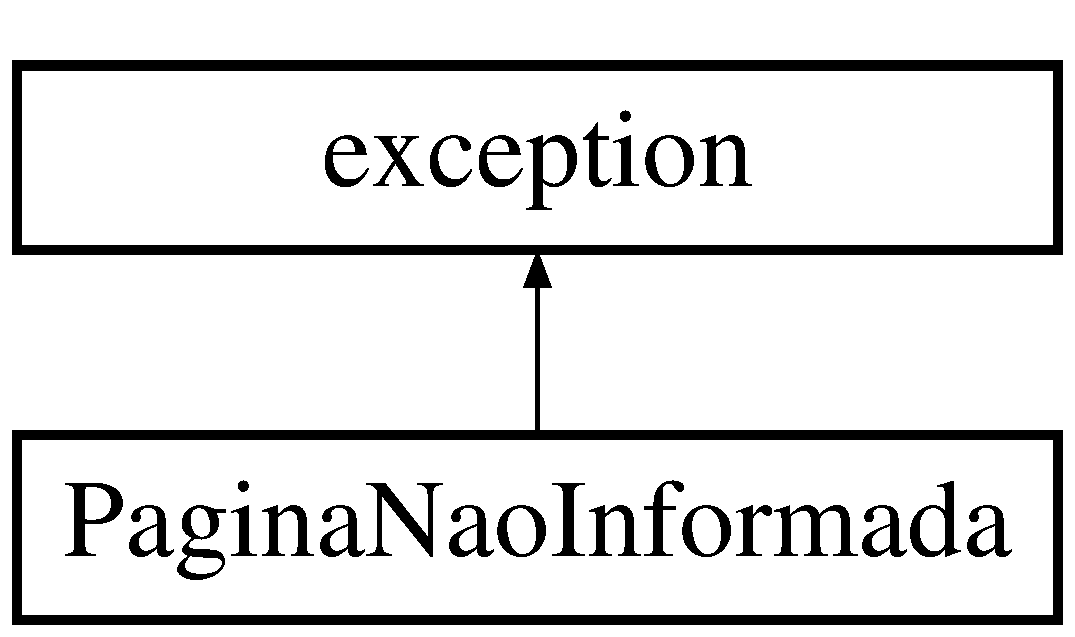
\includegraphics[height=2.000000cm]{classPaginaNaoInformada}
\end{center}
\end{figure}
\subsection*{Public Member Functions}
\begin{DoxyCompactItemize}
\item 
const char $\ast$ \hyperlink{classPaginaNaoInformada_a82d391c70c1e60f988448eac2b22571a}{what} () const noexcept override
\end{DoxyCompactItemize}
\subsection*{Private Attributes}
\begin{DoxyCompactItemize}
\item 
string \hyperlink{classPaginaNaoInformada_ac24c6f91d5c86702424530c6b0fba7ec}{mensagem} = \char`\"{}Você deve informar o número da página que deseja exibir. Tente novamente\char`\"{}
\end{DoxyCompactItemize}


\subsection{Member Function Documentation}
\mbox{\Hypertarget{classPaginaNaoInformada_a82d391c70c1e60f988448eac2b22571a}\label{classPaginaNaoInformada_a82d391c70c1e60f988448eac2b22571a}} 
\index{Pagina\+Nao\+Informada@{Pagina\+Nao\+Informada}!what@{what}}
\index{what@{what}!Pagina\+Nao\+Informada@{Pagina\+Nao\+Informada}}
\subsubsection{\texorpdfstring{what()}{what()}}
{\footnotesize\ttfamily const char$\ast$ Pagina\+Nao\+Informada\+::what (\begin{DoxyParamCaption}{ }\end{DoxyParamCaption}) const\hspace{0.3cm}{\ttfamily [inline]}, {\ttfamily [override]}, {\ttfamily [noexcept]}}



\subsection{Member Data Documentation}
\mbox{\Hypertarget{classPaginaNaoInformada_ac24c6f91d5c86702424530c6b0fba7ec}\label{classPaginaNaoInformada_ac24c6f91d5c86702424530c6b0fba7ec}} 
\index{Pagina\+Nao\+Informada@{Pagina\+Nao\+Informada}!mensagem@{mensagem}}
\index{mensagem@{mensagem}!Pagina\+Nao\+Informada@{Pagina\+Nao\+Informada}}
\subsubsection{\texorpdfstring{mensagem}{mensagem}}
{\footnotesize\ttfamily string Pagina\+Nao\+Informada\+::mensagem = \char`\"{}Você deve informar o número da página que deseja exibir. Tente novamente\char`\"{}\hspace{0.3cm}{\ttfamily [private]}}



The documentation for this class was generated from the following file\+:\begin{DoxyCompactItemize}
\item 
include/excecoes/\hyperlink{exc__pagina_8hpp}{exc\+\_\+pagina.\+hpp}\end{DoxyCompactItemize}

\hypertarget{classPrazoInvalido}{}\section{Prazo\+Invalido Class Reference}
\label{classPrazoInvalido}\index{Prazo\+Invalido@{Prazo\+Invalido}}


{\ttfamily \#include $<$exc\+\_\+tarefa.\+hpp$>$}

Inheritance diagram for Prazo\+Invalido\+:\begin{figure}[H]
\begin{center}
\leavevmode
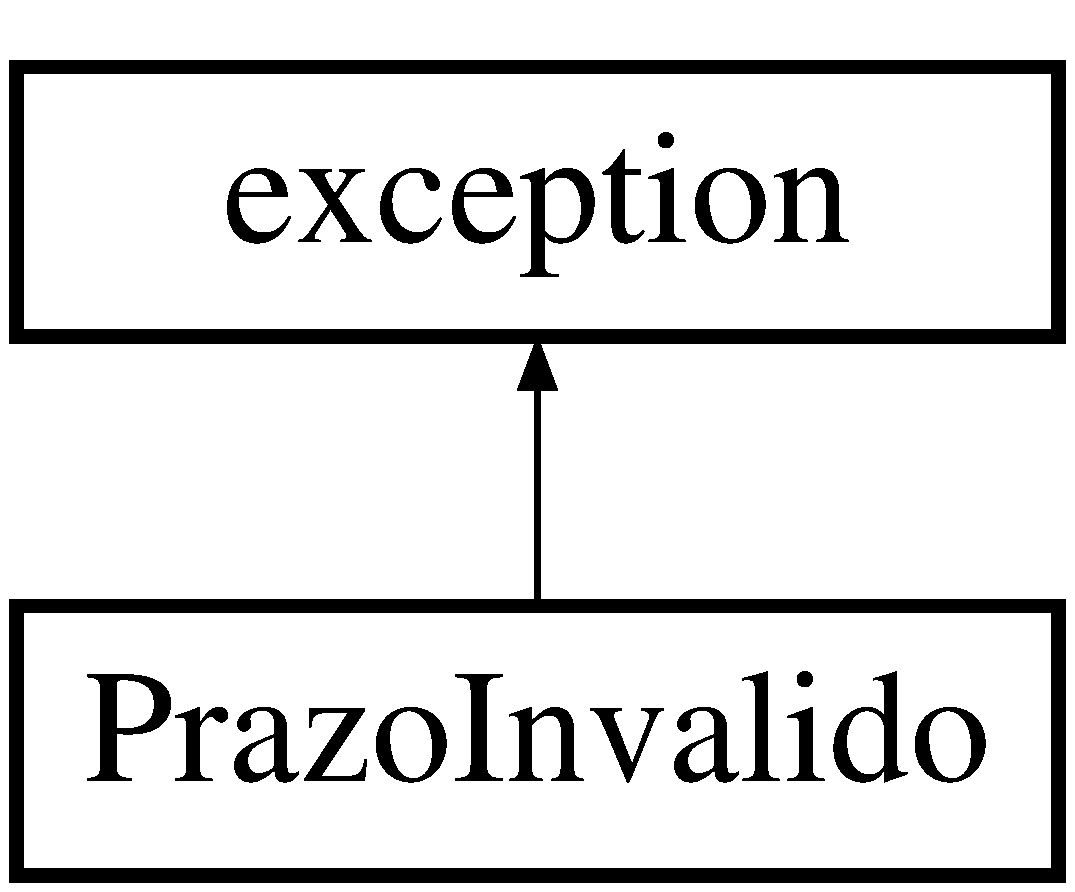
\includegraphics[height=2.000000cm]{classPrazoInvalido}
\end{center}
\end{figure}
\subsection*{Public Member Functions}
\begin{DoxyCompactItemize}
\item 
const char $\ast$ \hyperlink{classPrazoInvalido_a17083a87d16651f20e9f1aac6edcea4c}{what} () const noexcept override
\end{DoxyCompactItemize}
\subsection*{Private Attributes}
\begin{DoxyCompactItemize}
\item 
string \hyperlink{classPrazoInvalido_af2bb20a8cc0b09f0b348e0ea2f9d18e8}{mensagem} = \char`\"{}O prazo deve ter o formato \textquotesingle{}DD/MM/A\+A\+AA\textquotesingle{}. Tente novamente\char`\"{}
\end{DoxyCompactItemize}


\subsection{Member Function Documentation}
\mbox{\Hypertarget{classPrazoInvalido_a17083a87d16651f20e9f1aac6edcea4c}\label{classPrazoInvalido_a17083a87d16651f20e9f1aac6edcea4c}} 
\index{Prazo\+Invalido@{Prazo\+Invalido}!what@{what}}
\index{what@{what}!Prazo\+Invalido@{Prazo\+Invalido}}
\subsubsection{\texorpdfstring{what()}{what()}}
{\footnotesize\ttfamily const char$\ast$ Prazo\+Invalido\+::what (\begin{DoxyParamCaption}{ }\end{DoxyParamCaption}) const\hspace{0.3cm}{\ttfamily [inline]}, {\ttfamily [override]}, {\ttfamily [noexcept]}}



\subsection{Member Data Documentation}
\mbox{\Hypertarget{classPrazoInvalido_af2bb20a8cc0b09f0b348e0ea2f9d18e8}\label{classPrazoInvalido_af2bb20a8cc0b09f0b348e0ea2f9d18e8}} 
\index{Prazo\+Invalido@{Prazo\+Invalido}!mensagem@{mensagem}}
\index{mensagem@{mensagem}!Prazo\+Invalido@{Prazo\+Invalido}}
\subsubsection{\texorpdfstring{mensagem}{mensagem}}
{\footnotesize\ttfamily string Prazo\+Invalido\+::mensagem = \char`\"{}O prazo deve ter o formato \textquotesingle{}DD/MM/A\+A\+AA\textquotesingle{}. Tente novamente\char`\"{}\hspace{0.3cm}{\ttfamily [private]}}



The documentation for this class was generated from the following file\+:\begin{DoxyCompactItemize}
\item 
include/excecoes/\hyperlink{exc__tarefa_8hpp}{exc\+\_\+tarefa.\+hpp}\end{DoxyCompactItemize}

\hypertarget{classPrioridade}{}\section{Prioridade Class Reference}
\label{classPrioridade}\index{Prioridade@{Prioridade}}


{\ttfamily \#include $<$prioridade.\+hpp$>$}

Inheritance diagram for Prioridade\+:\begin{figure}[H]
\begin{center}
\leavevmode
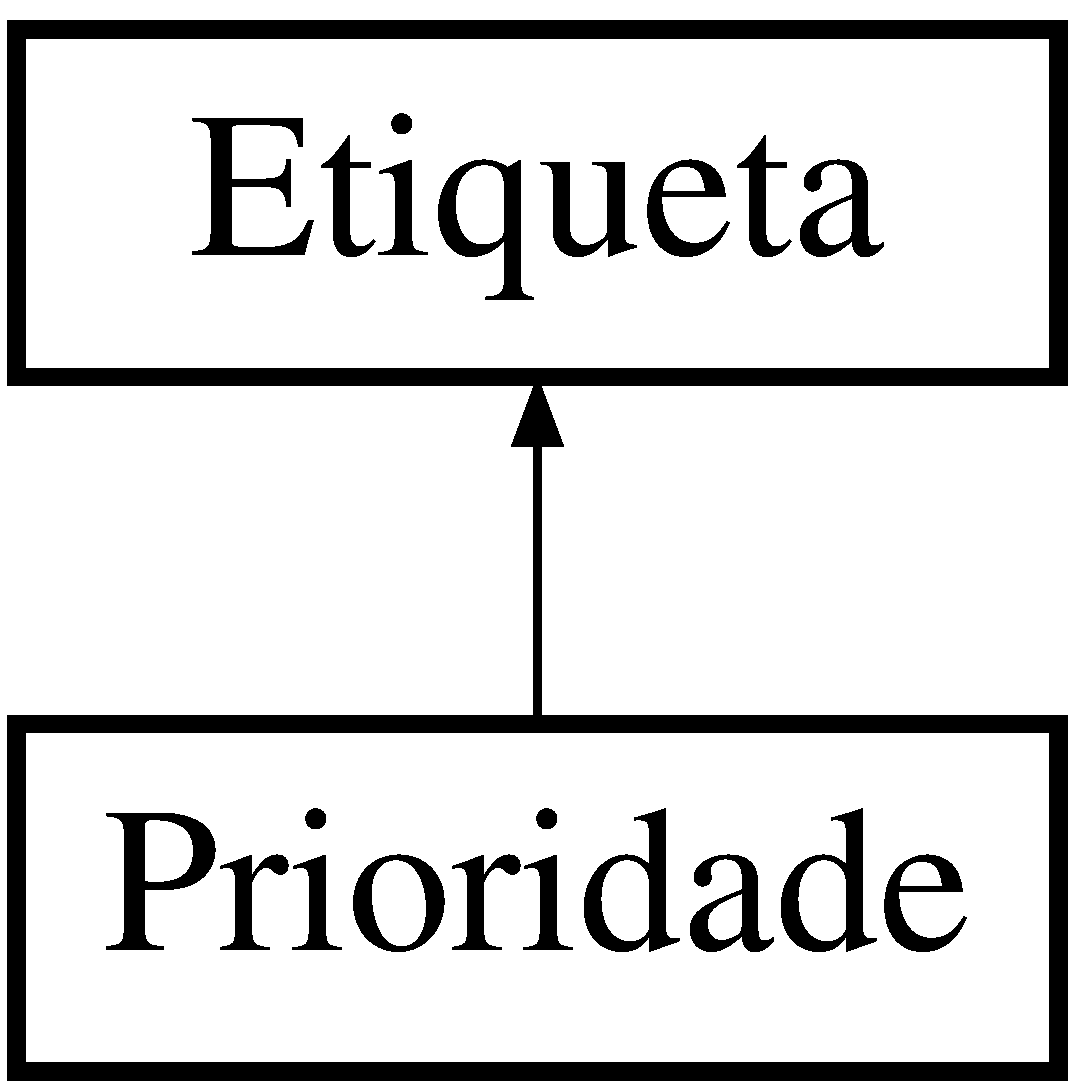
\includegraphics[height=2.000000cm]{classPrioridade}
\end{center}
\end{figure}
\subsection*{Public Member Functions}
\begin{DoxyCompactItemize}
\item 
\hyperlink{classPrioridade_adcad6f20e5c15a659968e088c8dd642e}{Prioridade} (string nome\+\_\+etiqueta, string tipo, int nivel\+\_\+prioridade)
\item 
int \hyperlink{classPrioridade_a9660b4662782a91b1061217f9122034a}{get\+\_\+nivel\+\_\+prioridade} ()
\item 
void \hyperlink{classPrioridade_ac9f930199df2060972b589c4f40ef3c7}{alterar\+\_\+valor} (int new\+\_\+prioridade)
\item 
string \hyperlink{classPrioridade_a01c961e447cff5a75d4400e6bcf59bb9}{get\+\_\+nome} ()
\item 
void \hyperlink{classPrioridade_a8457dcba4fb03aeb7ae5505d5d25226d}{editar\+\_\+prioridade} (string new\+\_\+nome)
\item 
void \hyperlink{classPrioridade_a8895aedea7a5c69c073d69e3dec802f6}{incrementa\+\_\+tarefa} ()
\end{DoxyCompactItemize}
\subsection*{Private Attributes}
\begin{DoxyCompactItemize}
\item 
int \hyperlink{classPrioridade_a33d58f99a6bab88419583a66b0a8e3b5}{\+\_\+nivel\+\_\+prioridade}
\end{DoxyCompactItemize}
\subsection*{Additional Inherited Members}


\subsection{Constructor \& Destructor Documentation}
\mbox{\Hypertarget{classPrioridade_adcad6f20e5c15a659968e088c8dd642e}\label{classPrioridade_adcad6f20e5c15a659968e088c8dd642e}} 
\index{Prioridade@{Prioridade}!Prioridade@{Prioridade}}
\index{Prioridade@{Prioridade}!Prioridade@{Prioridade}}
\subsubsection{\texorpdfstring{Prioridade()}{Prioridade()}}
{\footnotesize\ttfamily Prioridade\+::\+Prioridade (\begin{DoxyParamCaption}\item[{string}]{nome\+\_\+etiqueta,  }\item[{string}]{tipo,  }\item[{int}]{nivel\+\_\+prioridade }\end{DoxyParamCaption})}



\subsection{Member Function Documentation}
\mbox{\Hypertarget{classPrioridade_ac9f930199df2060972b589c4f40ef3c7}\label{classPrioridade_ac9f930199df2060972b589c4f40ef3c7}} 
\index{Prioridade@{Prioridade}!alterar\+\_\+valor@{alterar\+\_\+valor}}
\index{alterar\+\_\+valor@{alterar\+\_\+valor}!Prioridade@{Prioridade}}
\subsubsection{\texorpdfstring{alterar\+\_\+valor()}{alterar\_valor()}}
{\footnotesize\ttfamily void Prioridade\+::alterar\+\_\+valor (\begin{DoxyParamCaption}\item[{int}]{new\+\_\+prioridade }\end{DoxyParamCaption})}

\mbox{\Hypertarget{classPrioridade_a8457dcba4fb03aeb7ae5505d5d25226d}\label{classPrioridade_a8457dcba4fb03aeb7ae5505d5d25226d}} 
\index{Prioridade@{Prioridade}!editar\+\_\+prioridade@{editar\+\_\+prioridade}}
\index{editar\+\_\+prioridade@{editar\+\_\+prioridade}!Prioridade@{Prioridade}}
\subsubsection{\texorpdfstring{editar\+\_\+prioridade()}{editar\_prioridade()}}
{\footnotesize\ttfamily void Prioridade\+::editar\+\_\+prioridade (\begin{DoxyParamCaption}\item[{string}]{new\+\_\+nome }\end{DoxyParamCaption})}

\mbox{\Hypertarget{classPrioridade_a9660b4662782a91b1061217f9122034a}\label{classPrioridade_a9660b4662782a91b1061217f9122034a}} 
\index{Prioridade@{Prioridade}!get\+\_\+nivel\+\_\+prioridade@{get\+\_\+nivel\+\_\+prioridade}}
\index{get\+\_\+nivel\+\_\+prioridade@{get\+\_\+nivel\+\_\+prioridade}!Prioridade@{Prioridade}}
\subsubsection{\texorpdfstring{get\+\_\+nivel\+\_\+prioridade()}{get\_nivel\_prioridade()}}
{\footnotesize\ttfamily int Prioridade\+::get\+\_\+nivel\+\_\+prioridade (\begin{DoxyParamCaption}{ }\end{DoxyParamCaption})}

\mbox{\Hypertarget{classPrioridade_a01c961e447cff5a75d4400e6bcf59bb9}\label{classPrioridade_a01c961e447cff5a75d4400e6bcf59bb9}} 
\index{Prioridade@{Prioridade}!get\+\_\+nome@{get\+\_\+nome}}
\index{get\+\_\+nome@{get\+\_\+nome}!Prioridade@{Prioridade}}
\subsubsection{\texorpdfstring{get\+\_\+nome()}{get\_nome()}}
{\footnotesize\ttfamily string Prioridade\+::get\+\_\+nome (\begin{DoxyParamCaption}{ }\end{DoxyParamCaption})}

\mbox{\Hypertarget{classPrioridade_a8895aedea7a5c69c073d69e3dec802f6}\label{classPrioridade_a8895aedea7a5c69c073d69e3dec802f6}} 
\index{Prioridade@{Prioridade}!incrementa\+\_\+tarefa@{incrementa\+\_\+tarefa}}
\index{incrementa\+\_\+tarefa@{incrementa\+\_\+tarefa}!Prioridade@{Prioridade}}
\subsubsection{\texorpdfstring{incrementa\+\_\+tarefa()}{incrementa\_tarefa()}}
{\footnotesize\ttfamily void Prioridade\+::incrementa\+\_\+tarefa (\begin{DoxyParamCaption}{ }\end{DoxyParamCaption})}



\subsection{Member Data Documentation}
\mbox{\Hypertarget{classPrioridade_a33d58f99a6bab88419583a66b0a8e3b5}\label{classPrioridade_a33d58f99a6bab88419583a66b0a8e3b5}} 
\index{Prioridade@{Prioridade}!\+\_\+nivel\+\_\+prioridade@{\+\_\+nivel\+\_\+prioridade}}
\index{\+\_\+nivel\+\_\+prioridade@{\+\_\+nivel\+\_\+prioridade}!Prioridade@{Prioridade}}
\subsubsection{\texorpdfstring{\+\_\+nivel\+\_\+prioridade}{\_nivel\_prioridade}}
{\footnotesize\ttfamily int Prioridade\+::\+\_\+nivel\+\_\+prioridade\hspace{0.3cm}{\ttfamily [private]}}



The documentation for this class was generated from the following file\+:\begin{DoxyCompactItemize}
\item 
include/\hyperlink{prioridade_8hpp}{prioridade.\+hpp}\end{DoxyCompactItemize}

\hypertarget{classPrioridadeJaExiste}{}\section{Prioridade\+Ja\+Existe Class Reference}
\label{classPrioridadeJaExiste}\index{Prioridade\+Ja\+Existe@{Prioridade\+Ja\+Existe}}


{\ttfamily \#include $<$exc\+\_\+prioridade.\+hpp$>$}

Inheritance diagram for Prioridade\+Ja\+Existe\+:\begin{figure}[H]
\begin{center}
\leavevmode
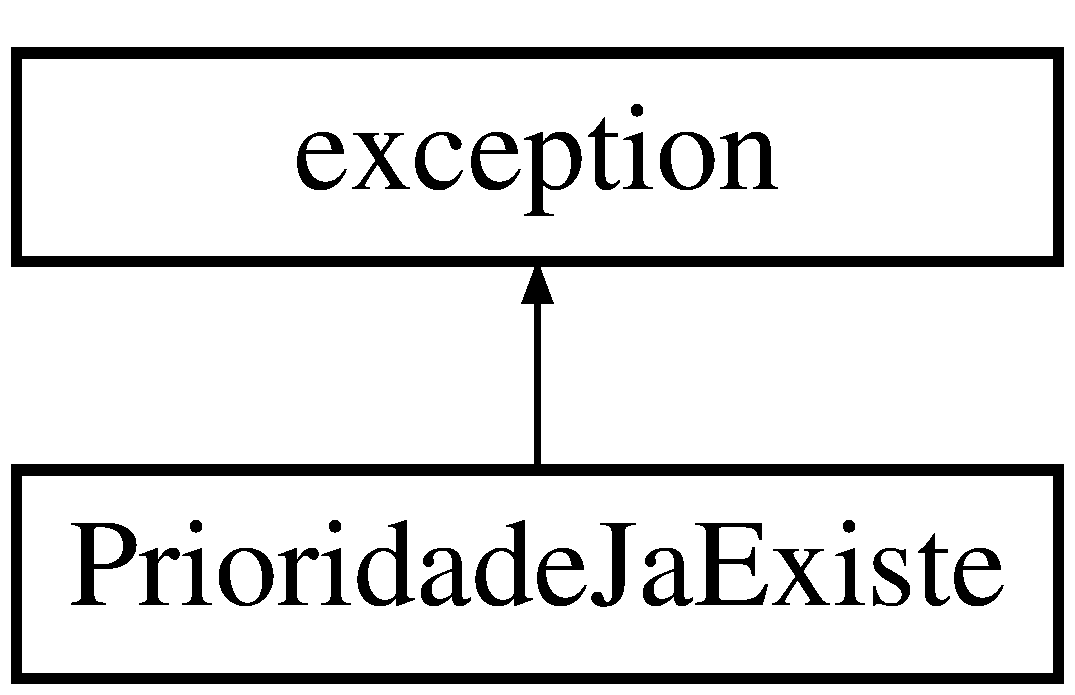
\includegraphics[height=2.000000cm]{classPrioridadeJaExiste}
\end{center}
\end{figure}
\subsection*{Public Member Functions}
\begin{DoxyCompactItemize}
\item 
const char $\ast$ \hyperlink{classPrioridadeJaExiste_aa2859fd1148802c4145ee579e04c1e7e}{what} () const noexcept override
\end{DoxyCompactItemize}
\subsection*{Private Attributes}
\begin{DoxyCompactItemize}
\item 
string \hyperlink{classPrioridadeJaExiste_aceee66510e48bda05955378f9e481104}{mensagem} = \char`\"{}Já existe uma prioridade com esse nome. Tente novamente\char`\"{}
\end{DoxyCompactItemize}


\subsection{Member Function Documentation}
\mbox{\Hypertarget{classPrioridadeJaExiste_aa2859fd1148802c4145ee579e04c1e7e}\label{classPrioridadeJaExiste_aa2859fd1148802c4145ee579e04c1e7e}} 
\index{Prioridade\+Ja\+Existe@{Prioridade\+Ja\+Existe}!what@{what}}
\index{what@{what}!Prioridade\+Ja\+Existe@{Prioridade\+Ja\+Existe}}
\subsubsection{\texorpdfstring{what()}{what()}}
{\footnotesize\ttfamily const char$\ast$ Prioridade\+Ja\+Existe\+::what (\begin{DoxyParamCaption}{ }\end{DoxyParamCaption}) const\hspace{0.3cm}{\ttfamily [inline]}, {\ttfamily [override]}, {\ttfamily [noexcept]}}



\subsection{Member Data Documentation}
\mbox{\Hypertarget{classPrioridadeJaExiste_aceee66510e48bda05955378f9e481104}\label{classPrioridadeJaExiste_aceee66510e48bda05955378f9e481104}} 
\index{Prioridade\+Ja\+Existe@{Prioridade\+Ja\+Existe}!mensagem@{mensagem}}
\index{mensagem@{mensagem}!Prioridade\+Ja\+Existe@{Prioridade\+Ja\+Existe}}
\subsubsection{\texorpdfstring{mensagem}{mensagem}}
{\footnotesize\ttfamily string Prioridade\+Ja\+Existe\+::mensagem = \char`\"{}Já existe uma prioridade com esse nome. Tente novamente\char`\"{}\hspace{0.3cm}{\ttfamily [private]}}



The documentation for this class was generated from the following file\+:\begin{DoxyCompactItemize}
\item 
include/excecoes/\hyperlink{exc__prioridade_8hpp}{exc\+\_\+prioridade.\+hpp}\end{DoxyCompactItemize}

\hypertarget{classPrioridadeNaoExiste}{}\section{Prioridade\+Nao\+Existe Class Reference}
\label{classPrioridadeNaoExiste}\index{Prioridade\+Nao\+Existe@{Prioridade\+Nao\+Existe}}


{\ttfamily \#include $<$exc\+\_\+prioridade.\+hpp$>$}

Inheritance diagram for Prioridade\+Nao\+Existe\+:\begin{figure}[H]
\begin{center}
\leavevmode
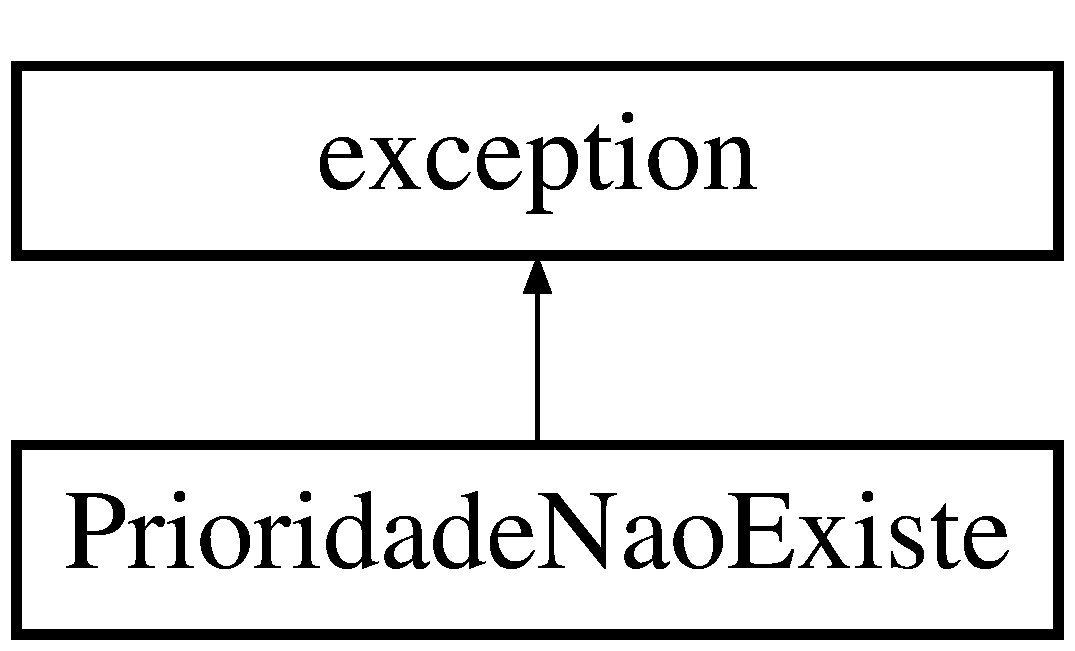
\includegraphics[height=2.000000cm]{classPrioridadeNaoExiste}
\end{center}
\end{figure}
\subsection*{Public Member Functions}
\begin{DoxyCompactItemize}
\item 
const char $\ast$ \hyperlink{classPrioridadeNaoExiste_a062cd6dd0326bc61a9505eab4cd78d4f}{what} () const noexcept override
\end{DoxyCompactItemize}
\subsection*{Private Attributes}
\begin{DoxyCompactItemize}
\item 
string \hyperlink{classPrioridadeNaoExiste_a5c675d0cd81b87bb26b6cac15b29cfb2}{mensagem} = \char`\"{}Não existe nenhuma prioridade com esse nome. Tente novamente\char`\"{}
\end{DoxyCompactItemize}


\subsection{Member Function Documentation}
\mbox{\Hypertarget{classPrioridadeNaoExiste_a062cd6dd0326bc61a9505eab4cd78d4f}\label{classPrioridadeNaoExiste_a062cd6dd0326bc61a9505eab4cd78d4f}} 
\index{Prioridade\+Nao\+Existe@{Prioridade\+Nao\+Existe}!what@{what}}
\index{what@{what}!Prioridade\+Nao\+Existe@{Prioridade\+Nao\+Existe}}
\subsubsection{\texorpdfstring{what()}{what()}}
{\footnotesize\ttfamily const char$\ast$ Prioridade\+Nao\+Existe\+::what (\begin{DoxyParamCaption}{ }\end{DoxyParamCaption}) const\hspace{0.3cm}{\ttfamily [inline]}, {\ttfamily [override]}, {\ttfamily [noexcept]}}



\subsection{Member Data Documentation}
\mbox{\Hypertarget{classPrioridadeNaoExiste_a5c675d0cd81b87bb26b6cac15b29cfb2}\label{classPrioridadeNaoExiste_a5c675d0cd81b87bb26b6cac15b29cfb2}} 
\index{Prioridade\+Nao\+Existe@{Prioridade\+Nao\+Existe}!mensagem@{mensagem}}
\index{mensagem@{mensagem}!Prioridade\+Nao\+Existe@{Prioridade\+Nao\+Existe}}
\subsubsection{\texorpdfstring{mensagem}{mensagem}}
{\footnotesize\ttfamily string Prioridade\+Nao\+Existe\+::mensagem = \char`\"{}Não existe nenhuma prioridade com esse nome. Tente novamente\char`\"{}\hspace{0.3cm}{\ttfamily [private]}}



The documentation for this class was generated from the following file\+:\begin{DoxyCompactItemize}
\item 
include/excecoes/\hyperlink{exc__prioridade_8hpp}{exc\+\_\+prioridade.\+hpp}\end{DoxyCompactItemize}

\hypertarget{classSenhaIncorreta}{}\section{Senha\+Incorreta Class Reference}
\label{classSenhaIncorreta}\index{Senha\+Incorreta@{Senha\+Incorreta}}


{\ttfamily \#include $<$exc\+\_\+usuario.\+hpp$>$}

Inheritance diagram for Senha\+Incorreta\+:\begin{figure}[H]
\begin{center}
\leavevmode
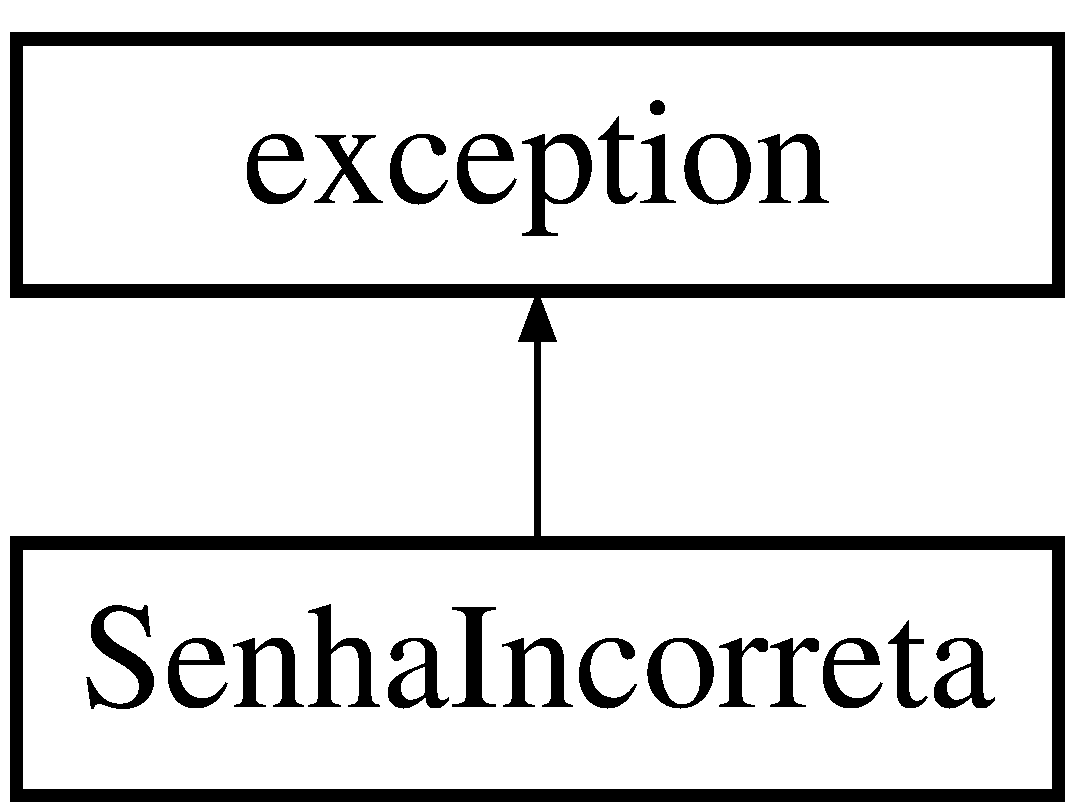
\includegraphics[height=2.000000cm]{classSenhaIncorreta}
\end{center}
\end{figure}
\subsection*{Public Member Functions}
\begin{DoxyCompactItemize}
\item 
const char $\ast$ \hyperlink{classSenhaIncorreta_a88aa7d851d1f6e81ef29f5ce3bae0c76}{what} () const noexcept override
\end{DoxyCompactItemize}
\subsection*{Private Attributes}
\begin{DoxyCompactItemize}
\item 
string \hyperlink{classSenhaIncorreta_a79a5b7430df661579c81fd1be29ff66f}{mensagem} = \char`\"{}Senha incorreta. Tente novamente.\char`\"{}
\end{DoxyCompactItemize}


\subsection{Member Function Documentation}
\mbox{\Hypertarget{classSenhaIncorreta_a88aa7d851d1f6e81ef29f5ce3bae0c76}\label{classSenhaIncorreta_a88aa7d851d1f6e81ef29f5ce3bae0c76}} 
\index{Senha\+Incorreta@{Senha\+Incorreta}!what@{what}}
\index{what@{what}!Senha\+Incorreta@{Senha\+Incorreta}}
\subsubsection{\texorpdfstring{what()}{what()}}
{\footnotesize\ttfamily const char$\ast$ Senha\+Incorreta\+::what (\begin{DoxyParamCaption}{ }\end{DoxyParamCaption}) const\hspace{0.3cm}{\ttfamily [inline]}, {\ttfamily [override]}, {\ttfamily [noexcept]}}



\subsection{Member Data Documentation}
\mbox{\Hypertarget{classSenhaIncorreta_a79a5b7430df661579c81fd1be29ff66f}\label{classSenhaIncorreta_a79a5b7430df661579c81fd1be29ff66f}} 
\index{Senha\+Incorreta@{Senha\+Incorreta}!mensagem@{mensagem}}
\index{mensagem@{mensagem}!Senha\+Incorreta@{Senha\+Incorreta}}
\subsubsection{\texorpdfstring{mensagem}{mensagem}}
{\footnotesize\ttfamily string Senha\+Incorreta\+::mensagem = \char`\"{}Senha incorreta. Tente novamente.\char`\"{}\hspace{0.3cm}{\ttfamily [private]}}



The documentation for this class was generated from the following file\+:\begin{DoxyCompactItemize}
\item 
include/excecoes/\hyperlink{exc__usuario_8hpp}{exc\+\_\+usuario.\+hpp}\end{DoxyCompactItemize}

\hypertarget{classStorage}{}\section{Storage Class Reference}
\label{classStorage}\index{Storage@{Storage}}


{\ttfamily \#include $<$storage.\+hpp$>$}

\subsection*{Public Member Functions}
\begin{DoxyCompactItemize}
\item 
\hyperlink{classStorage_a80ef6af5e4c9fd4424ae16e808d05291}{Storage} ()
\item 
string \hyperlink{classStorage_a72004c148e48fdd5fde71db2319762e9}{get\+\_\+nome\+\_\+arquivo} (string usuario)
\item 
bool \hyperlink{classStorage_adb9fc5565d70a106da231654e15cf090}{usuario\+\_\+existe} (string usuario)
\item 
void \hyperlink{classStorage_a572d1e337404b8819f1565be9689a271}{cria\+\_\+usuario} (string usuario, string senha)
\item 
bool \hyperlink{classStorage_af2d39c70a0cd9d63959ab90c9f039dee}{confere\+\_\+senha} (string usuario, string senha)
\item 
void \hyperlink{classStorage_a4d149db70dfa838a52ad53bb22555050}{ordena\+\_\+tarefas} ()
\item 
void \hyperlink{classStorage_a0b13d6c7e111f6bbeb4c6c03feb532c9}{le\+\_\+tarefa} ()
\item 
void \hyperlink{classStorage_a571f009d0dca33811883d381a70ccda5}{le\+\_\+grupo} ()
\item 
void \hyperlink{classStorage_aac1b536c28c1bd7a3bef1f0b8738f8d2}{le\+\_\+prioridade} ()
\item 
void \hyperlink{classStorage_a2e74fd83ed4bcaad391af72e8cd569c1}{le\+\_\+conteudo} ()
\item 
int \hyperlink{classStorage_aa42ca5fe247fbc390ca86c4a05346daa}{get\+\_\+qtd\+\_\+tarefas} ()
\item 
int \hyperlink{classStorage_ae92552f01f0e393d4168f6e159a0ca12}{get\+\_\+qtd\+\_\+grupos} ()
\item 
int \hyperlink{classStorage_a3ab42001bc5be1d4607fb5b24157c85d}{get\+\_\+qtd\+\_\+prioridades} ()
\item 
\hyperlink{classPrioridade}{Prioridade} $\ast$ \hyperlink{classStorage_aeb09b13da8b70a5bc279197d7298de06}{get\+\_\+prioridade} (string nome\+\_\+prioridade)
\item 
\hyperlink{classPrioridade}{Prioridade} $\ast$ \hyperlink{classStorage_abc3618c3a0b69ffe6e895cd701b0516e}{get\+\_\+prioridade} (int indice\+\_\+prioridade)
\item 
\hyperlink{classGrupo}{Grupo} $\ast$ \hyperlink{classStorage_a1b478e593dd0b18eeb7fc0490b87b362}{get\+\_\+grupo} (string nome\+\_\+grupo)
\item 
\hyperlink{classGrupo}{Grupo} $\ast$ \hyperlink{classStorage_af340fa785af6416b6d7ca0eb38ea4be7}{get\+\_\+grupo} (int indice\+\_\+grupo)
\item 
\hyperlink{classTarefa}{Tarefa} $\ast$ \hyperlink{classStorage_af8f0367791223137d6249220bceb4d22}{get\+\_\+tarefa} (string titulo\+\_\+tarefa)
\item 
\hyperlink{classTarefa}{Tarefa} $\ast$ \hyperlink{classStorage_ae1d09a603b179fe84c9d4e1dfa02e4cb}{get\+\_\+tarefa} (int indice\+\_\+tarefa)
\item 
void \hyperlink{classStorage_a128d891f8907c1089e8ac925743b0446}{registra\+\_\+tarefa} (\hyperlink{classTarefa}{Tarefa} $\ast$tarefa)
\item 
void \hyperlink{classStorage_a53b5c543a7eb6ca4bb7a83433b67e977}{cria\+\_\+tarefa} (string titulo, string descricao, string prazo, string grupo\+\_\+tarefa, string prioridade\+\_\+tarefa)
\item 
void \hyperlink{classStorage_a566777194a365ed00d442ec3d531e146}{registra\+\_\+grupo} (\hyperlink{classGrupo}{Grupo} $\ast$grupo)
\item 
void \hyperlink{classStorage_ae08fbaf921bcbbd0b92da839ff930e76}{cria\+\_\+grupo} (string nome\+\_\+etiqueta, string descricao)
\item 
void \hyperlink{classStorage_a203e5aad2fc6a8fbd4a23b37c4cb9f3c}{registra\+\_\+prioridade} (\hyperlink{classPrioridade}{Prioridade} $\ast$prioridade)
\item 
void \hyperlink{classStorage_a2cb353c0910afe7c69996b51dc65a754}{cria\+\_\+prioridade} (string nome\+\_\+etiqueta, int nivel\+\_\+prioridade)
\item 
bool \hyperlink{classStorage_a501b15eb866bfbc27aa968ce96b8ae8b}{tarefa\+\_\+existe} (string titulo\+\_\+tarefa)
\item 
bool \hyperlink{classStorage_a7d38af18bdb46b1c8928cdadca13db52}{grupo\+\_\+existe} (string nome\+\_\+grupo)
\item 
bool \hyperlink{classStorage_aaa42cd171fb2624c9675e2b220d532e4}{prioridade\+\_\+existe} (string nome\+\_\+prioridade)
\item 
void \hyperlink{classStorage_a6164e94fc3a86249dcce0aa66320ad2b}{editar\+\_\+titulo} (int indice\+\_\+tarefa, string novo\+\_\+titulo)
\item 
void \hyperlink{classStorage_aca052dc1a570f55746a66f1dd7795354}{editar\+\_\+descricao} (int indice\+\_\+tarefa, string nova\+\_\+descricao)
\item 
void \hyperlink{classStorage_a593548cb2b9ee3e570dae32b55140a0c}{editar\+\_\+prazo} (int indice\+\_\+tarefa, string novo\+\_\+prazo)
\item 
void \hyperlink{classStorage_a34a852bccbf913731f17a654e6e97c5a}{editar\+\_\+grupo} (int indice\+\_\+tarefa, string novo\+\_\+grupo)
\item 
void \hyperlink{classStorage_a15c3a41053de23043a4b16c751515804}{editar\+\_\+prioridade} (int indice\+\_\+tarefa, string nova\+\_\+prioridade)
\item 
void \hyperlink{classStorage_a9ffb7a7dad34dc12d3dc4e6808e5f431}{alterar\+\_\+grupo} (int indice\+\_\+grupo, string novo\+\_\+grupo)
\item 
void \hyperlink{classStorage_af487be83a5acaf49850f9fff02e0e30f}{alterar\+\_\+des\+\_\+grupo} (int indice\+\_\+grupo, string nova\+\_\+descricao)
\item 
void \hyperlink{classStorage_aad0905f797b2112aa95846bbb1714873}{alterar\+\_\+prioridade} (int indice\+\_\+prioridade, string nova\+\_\+prioridade)
\item 
void \hyperlink{classStorage_a3e7f675101378565f4f63d799e8408ae}{alterar\+\_\+nivel} (int indice\+\_\+prioridade, int novo\+\_\+nivel)
\item 
void \hyperlink{classStorage_acd2ad4c9120d2968cb811be2d96ce7ea}{alterar\+\_\+concluido} (int indice\+\_\+tarefa, bool novo\+\_\+status)
\item 
void \hyperlink{classStorage_a2b6c4db3728ad5f6f9787b7af199b4a0}{apaga\+\_\+tarefa} (int indice\+\_\+tarefa)
\item 
void \hyperlink{classStorage_abf9179dcd9d27a8e1b5faf74d254f1bb}{apaga\+\_\+grupo} (int indice\+\_\+grupo)
\item 
void \hyperlink{classStorage_ac05b88b868646f514f2c8c114c28ce60}{apaga\+\_\+prioridade} (int indice\+\_\+prioridade)
\end{DoxyCompactItemize}
\subsection*{Private Attributes}
\begin{DoxyCompactItemize}
\item 
fstream \hyperlink{classStorage_ad9934ed8b6423a91135819a7f301ffba}{\+\_\+file}
\item 
bool \hyperlink{classStorage_afb88caad0d6b81083c03169d39718f81}{\+\_\+logado}
\item 
string \hyperlink{classStorage_a2c715507a5c7b44e912a827faf310dc8}{\+\_\+usuario\+\_\+logado}
\item 
vector$<$ \hyperlink{classTarefa}{Tarefa} $\ast$ $>$ \hyperlink{classStorage_a289eb400729d4db505aa427cdcd83fdf}{\+\_\+tarefas}
\item 
vector$<$ \hyperlink{classGrupo}{Grupo} $\ast$ $>$ \hyperlink{classStorage_a4bd9a86ddbe7dd8d4f2a2b0fe60255e6}{\+\_\+grupos}
\item 
vector$<$ \hyperlink{classPrioridade}{Prioridade} $\ast$ $>$ \hyperlink{classStorage_a1cd2e4e622c1e7988c8bc52f2a56f869}{\+\_\+prioridades}
\end{DoxyCompactItemize}


\subsection{Constructor \& Destructor Documentation}
\mbox{\Hypertarget{classStorage_a80ef6af5e4c9fd4424ae16e808d05291}\label{classStorage_a80ef6af5e4c9fd4424ae16e808d05291}} 
\index{Storage@{Storage}!Storage@{Storage}}
\index{Storage@{Storage}!Storage@{Storage}}
\subsubsection{\texorpdfstring{Storage()}{Storage()}}
{\footnotesize\ttfamily Storage\+::\+Storage (\begin{DoxyParamCaption}{ }\end{DoxyParamCaption})}



\subsection{Member Function Documentation}
\mbox{\Hypertarget{classStorage_acd2ad4c9120d2968cb811be2d96ce7ea}\label{classStorage_acd2ad4c9120d2968cb811be2d96ce7ea}} 
\index{Storage@{Storage}!alterar\+\_\+concluido@{alterar\+\_\+concluido}}
\index{alterar\+\_\+concluido@{alterar\+\_\+concluido}!Storage@{Storage}}
\subsubsection{\texorpdfstring{alterar\+\_\+concluido()}{alterar\_concluido()}}
{\footnotesize\ttfamily void Storage\+::alterar\+\_\+concluido (\begin{DoxyParamCaption}\item[{int}]{indice\+\_\+tarefa,  }\item[{bool}]{novo\+\_\+status }\end{DoxyParamCaption})}

\mbox{\Hypertarget{classStorage_af487be83a5acaf49850f9fff02e0e30f}\label{classStorage_af487be83a5acaf49850f9fff02e0e30f}} 
\index{Storage@{Storage}!alterar\+\_\+des\+\_\+grupo@{alterar\+\_\+des\+\_\+grupo}}
\index{alterar\+\_\+des\+\_\+grupo@{alterar\+\_\+des\+\_\+grupo}!Storage@{Storage}}
\subsubsection{\texorpdfstring{alterar\+\_\+des\+\_\+grupo()}{alterar\_des\_grupo()}}
{\footnotesize\ttfamily void Storage\+::alterar\+\_\+des\+\_\+grupo (\begin{DoxyParamCaption}\item[{int}]{indice\+\_\+grupo,  }\item[{string}]{nova\+\_\+descricao }\end{DoxyParamCaption})}

\mbox{\Hypertarget{classStorage_a9ffb7a7dad34dc12d3dc4e6808e5f431}\label{classStorage_a9ffb7a7dad34dc12d3dc4e6808e5f431}} 
\index{Storage@{Storage}!alterar\+\_\+grupo@{alterar\+\_\+grupo}}
\index{alterar\+\_\+grupo@{alterar\+\_\+grupo}!Storage@{Storage}}
\subsubsection{\texorpdfstring{alterar\+\_\+grupo()}{alterar\_grupo()}}
{\footnotesize\ttfamily void Storage\+::alterar\+\_\+grupo (\begin{DoxyParamCaption}\item[{int}]{indice\+\_\+grupo,  }\item[{string}]{novo\+\_\+grupo }\end{DoxyParamCaption})}

\mbox{\Hypertarget{classStorage_a3e7f675101378565f4f63d799e8408ae}\label{classStorage_a3e7f675101378565f4f63d799e8408ae}} 
\index{Storage@{Storage}!alterar\+\_\+nivel@{alterar\+\_\+nivel}}
\index{alterar\+\_\+nivel@{alterar\+\_\+nivel}!Storage@{Storage}}
\subsubsection{\texorpdfstring{alterar\+\_\+nivel()}{alterar\_nivel()}}
{\footnotesize\ttfamily void Storage\+::alterar\+\_\+nivel (\begin{DoxyParamCaption}\item[{int}]{indice\+\_\+prioridade,  }\item[{int}]{novo\+\_\+nivel }\end{DoxyParamCaption})}

\mbox{\Hypertarget{classStorage_aad0905f797b2112aa95846bbb1714873}\label{classStorage_aad0905f797b2112aa95846bbb1714873}} 
\index{Storage@{Storage}!alterar\+\_\+prioridade@{alterar\+\_\+prioridade}}
\index{alterar\+\_\+prioridade@{alterar\+\_\+prioridade}!Storage@{Storage}}
\subsubsection{\texorpdfstring{alterar\+\_\+prioridade()}{alterar\_prioridade()}}
{\footnotesize\ttfamily void Storage\+::alterar\+\_\+prioridade (\begin{DoxyParamCaption}\item[{int}]{indice\+\_\+prioridade,  }\item[{string}]{nova\+\_\+prioridade }\end{DoxyParamCaption})}

\mbox{\Hypertarget{classStorage_abf9179dcd9d27a8e1b5faf74d254f1bb}\label{classStorage_abf9179dcd9d27a8e1b5faf74d254f1bb}} 
\index{Storage@{Storage}!apaga\+\_\+grupo@{apaga\+\_\+grupo}}
\index{apaga\+\_\+grupo@{apaga\+\_\+grupo}!Storage@{Storage}}
\subsubsection{\texorpdfstring{apaga\+\_\+grupo()}{apaga\_grupo()}}
{\footnotesize\ttfamily void Storage\+::apaga\+\_\+grupo (\begin{DoxyParamCaption}\item[{int}]{indice\+\_\+grupo }\end{DoxyParamCaption})}

\mbox{\Hypertarget{classStorage_ac05b88b868646f514f2c8c114c28ce60}\label{classStorage_ac05b88b868646f514f2c8c114c28ce60}} 
\index{Storage@{Storage}!apaga\+\_\+prioridade@{apaga\+\_\+prioridade}}
\index{apaga\+\_\+prioridade@{apaga\+\_\+prioridade}!Storage@{Storage}}
\subsubsection{\texorpdfstring{apaga\+\_\+prioridade()}{apaga\_prioridade()}}
{\footnotesize\ttfamily void Storage\+::apaga\+\_\+prioridade (\begin{DoxyParamCaption}\item[{int}]{indice\+\_\+prioridade }\end{DoxyParamCaption})}

\mbox{\Hypertarget{classStorage_a2b6c4db3728ad5f6f9787b7af199b4a0}\label{classStorage_a2b6c4db3728ad5f6f9787b7af199b4a0}} 
\index{Storage@{Storage}!apaga\+\_\+tarefa@{apaga\+\_\+tarefa}}
\index{apaga\+\_\+tarefa@{apaga\+\_\+tarefa}!Storage@{Storage}}
\subsubsection{\texorpdfstring{apaga\+\_\+tarefa()}{apaga\_tarefa()}}
{\footnotesize\ttfamily void Storage\+::apaga\+\_\+tarefa (\begin{DoxyParamCaption}\item[{int}]{indice\+\_\+tarefa }\end{DoxyParamCaption})}

\mbox{\Hypertarget{classStorage_af2d39c70a0cd9d63959ab90c9f039dee}\label{classStorage_af2d39c70a0cd9d63959ab90c9f039dee}} 
\index{Storage@{Storage}!confere\+\_\+senha@{confere\+\_\+senha}}
\index{confere\+\_\+senha@{confere\+\_\+senha}!Storage@{Storage}}
\subsubsection{\texorpdfstring{confere\+\_\+senha()}{confere\_senha()}}
{\footnotesize\ttfamily bool Storage\+::confere\+\_\+senha (\begin{DoxyParamCaption}\item[{string}]{usuario,  }\item[{string}]{senha }\end{DoxyParamCaption})}

\mbox{\Hypertarget{classStorage_ae08fbaf921bcbbd0b92da839ff930e76}\label{classStorage_ae08fbaf921bcbbd0b92da839ff930e76}} 
\index{Storage@{Storage}!cria\+\_\+grupo@{cria\+\_\+grupo}}
\index{cria\+\_\+grupo@{cria\+\_\+grupo}!Storage@{Storage}}
\subsubsection{\texorpdfstring{cria\+\_\+grupo()}{cria\_grupo()}}
{\footnotesize\ttfamily void Storage\+::cria\+\_\+grupo (\begin{DoxyParamCaption}\item[{string}]{nome\+\_\+etiqueta,  }\item[{string}]{descricao }\end{DoxyParamCaption})}

\mbox{\Hypertarget{classStorage_a2cb353c0910afe7c69996b51dc65a754}\label{classStorage_a2cb353c0910afe7c69996b51dc65a754}} 
\index{Storage@{Storage}!cria\+\_\+prioridade@{cria\+\_\+prioridade}}
\index{cria\+\_\+prioridade@{cria\+\_\+prioridade}!Storage@{Storage}}
\subsubsection{\texorpdfstring{cria\+\_\+prioridade()}{cria\_prioridade()}}
{\footnotesize\ttfamily void Storage\+::cria\+\_\+prioridade (\begin{DoxyParamCaption}\item[{string}]{nome\+\_\+etiqueta,  }\item[{int}]{nivel\+\_\+prioridade }\end{DoxyParamCaption})}

\mbox{\Hypertarget{classStorage_a53b5c543a7eb6ca4bb7a83433b67e977}\label{classStorage_a53b5c543a7eb6ca4bb7a83433b67e977}} 
\index{Storage@{Storage}!cria\+\_\+tarefa@{cria\+\_\+tarefa}}
\index{cria\+\_\+tarefa@{cria\+\_\+tarefa}!Storage@{Storage}}
\subsubsection{\texorpdfstring{cria\+\_\+tarefa()}{cria\_tarefa()}}
{\footnotesize\ttfamily void Storage\+::cria\+\_\+tarefa (\begin{DoxyParamCaption}\item[{string}]{titulo,  }\item[{string}]{descricao,  }\item[{string}]{prazo,  }\item[{string}]{grupo\+\_\+tarefa,  }\item[{string}]{prioridade\+\_\+tarefa }\end{DoxyParamCaption})}

\mbox{\Hypertarget{classStorage_a572d1e337404b8819f1565be9689a271}\label{classStorage_a572d1e337404b8819f1565be9689a271}} 
\index{Storage@{Storage}!cria\+\_\+usuario@{cria\+\_\+usuario}}
\index{cria\+\_\+usuario@{cria\+\_\+usuario}!Storage@{Storage}}
\subsubsection{\texorpdfstring{cria\+\_\+usuario()}{cria\_usuario()}}
{\footnotesize\ttfamily void Storage\+::cria\+\_\+usuario (\begin{DoxyParamCaption}\item[{string}]{usuario,  }\item[{string}]{senha }\end{DoxyParamCaption})}

\mbox{\Hypertarget{classStorage_aca052dc1a570f55746a66f1dd7795354}\label{classStorage_aca052dc1a570f55746a66f1dd7795354}} 
\index{Storage@{Storage}!editar\+\_\+descricao@{editar\+\_\+descricao}}
\index{editar\+\_\+descricao@{editar\+\_\+descricao}!Storage@{Storage}}
\subsubsection{\texorpdfstring{editar\+\_\+descricao()}{editar\_descricao()}}
{\footnotesize\ttfamily void Storage\+::editar\+\_\+descricao (\begin{DoxyParamCaption}\item[{int}]{indice\+\_\+tarefa,  }\item[{string}]{nova\+\_\+descricao }\end{DoxyParamCaption})}

\mbox{\Hypertarget{classStorage_a34a852bccbf913731f17a654e6e97c5a}\label{classStorage_a34a852bccbf913731f17a654e6e97c5a}} 
\index{Storage@{Storage}!editar\+\_\+grupo@{editar\+\_\+grupo}}
\index{editar\+\_\+grupo@{editar\+\_\+grupo}!Storage@{Storage}}
\subsubsection{\texorpdfstring{editar\+\_\+grupo()}{editar\_grupo()}}
{\footnotesize\ttfamily void Storage\+::editar\+\_\+grupo (\begin{DoxyParamCaption}\item[{int}]{indice\+\_\+tarefa,  }\item[{string}]{novo\+\_\+grupo }\end{DoxyParamCaption})}

\mbox{\Hypertarget{classStorage_a593548cb2b9ee3e570dae32b55140a0c}\label{classStorage_a593548cb2b9ee3e570dae32b55140a0c}} 
\index{Storage@{Storage}!editar\+\_\+prazo@{editar\+\_\+prazo}}
\index{editar\+\_\+prazo@{editar\+\_\+prazo}!Storage@{Storage}}
\subsubsection{\texorpdfstring{editar\+\_\+prazo()}{editar\_prazo()}}
{\footnotesize\ttfamily void Storage\+::editar\+\_\+prazo (\begin{DoxyParamCaption}\item[{int}]{indice\+\_\+tarefa,  }\item[{string}]{novo\+\_\+prazo }\end{DoxyParamCaption})}

\mbox{\Hypertarget{classStorage_a15c3a41053de23043a4b16c751515804}\label{classStorage_a15c3a41053de23043a4b16c751515804}} 
\index{Storage@{Storage}!editar\+\_\+prioridade@{editar\+\_\+prioridade}}
\index{editar\+\_\+prioridade@{editar\+\_\+prioridade}!Storage@{Storage}}
\subsubsection{\texorpdfstring{editar\+\_\+prioridade()}{editar\_prioridade()}}
{\footnotesize\ttfamily void Storage\+::editar\+\_\+prioridade (\begin{DoxyParamCaption}\item[{int}]{indice\+\_\+tarefa,  }\item[{string}]{nova\+\_\+prioridade }\end{DoxyParamCaption})}

\mbox{\Hypertarget{classStorage_a6164e94fc3a86249dcce0aa66320ad2b}\label{classStorage_a6164e94fc3a86249dcce0aa66320ad2b}} 
\index{Storage@{Storage}!editar\+\_\+titulo@{editar\+\_\+titulo}}
\index{editar\+\_\+titulo@{editar\+\_\+titulo}!Storage@{Storage}}
\subsubsection{\texorpdfstring{editar\+\_\+titulo()}{editar\_titulo()}}
{\footnotesize\ttfamily void Storage\+::editar\+\_\+titulo (\begin{DoxyParamCaption}\item[{int}]{indice\+\_\+tarefa,  }\item[{string}]{novo\+\_\+titulo }\end{DoxyParamCaption})}

\mbox{\Hypertarget{classStorage_a1b478e593dd0b18eeb7fc0490b87b362}\label{classStorage_a1b478e593dd0b18eeb7fc0490b87b362}} 
\index{Storage@{Storage}!get\+\_\+grupo@{get\+\_\+grupo}}
\index{get\+\_\+grupo@{get\+\_\+grupo}!Storage@{Storage}}
\subsubsection{\texorpdfstring{get\+\_\+grupo()}{get\_grupo()}\hspace{0.1cm}{\footnotesize\ttfamily [1/2]}}
{\footnotesize\ttfamily \hyperlink{classGrupo}{Grupo}$\ast$ Storage\+::get\+\_\+grupo (\begin{DoxyParamCaption}\item[{string}]{nome\+\_\+grupo }\end{DoxyParamCaption})}

\mbox{\Hypertarget{classStorage_af340fa785af6416b6d7ca0eb38ea4be7}\label{classStorage_af340fa785af6416b6d7ca0eb38ea4be7}} 
\index{Storage@{Storage}!get\+\_\+grupo@{get\+\_\+grupo}}
\index{get\+\_\+grupo@{get\+\_\+grupo}!Storage@{Storage}}
\subsubsection{\texorpdfstring{get\+\_\+grupo()}{get\_grupo()}\hspace{0.1cm}{\footnotesize\ttfamily [2/2]}}
{\footnotesize\ttfamily \hyperlink{classGrupo}{Grupo}$\ast$ Storage\+::get\+\_\+grupo (\begin{DoxyParamCaption}\item[{int}]{indice\+\_\+grupo }\end{DoxyParamCaption})}

\mbox{\Hypertarget{classStorage_a72004c148e48fdd5fde71db2319762e9}\label{classStorage_a72004c148e48fdd5fde71db2319762e9}} 
\index{Storage@{Storage}!get\+\_\+nome\+\_\+arquivo@{get\+\_\+nome\+\_\+arquivo}}
\index{get\+\_\+nome\+\_\+arquivo@{get\+\_\+nome\+\_\+arquivo}!Storage@{Storage}}
\subsubsection{\texorpdfstring{get\+\_\+nome\+\_\+arquivo()}{get\_nome\_arquivo()}}
{\footnotesize\ttfamily string Storage\+::get\+\_\+nome\+\_\+arquivo (\begin{DoxyParamCaption}\item[{string}]{usuario }\end{DoxyParamCaption})}

\mbox{\Hypertarget{classStorage_aeb09b13da8b70a5bc279197d7298de06}\label{classStorage_aeb09b13da8b70a5bc279197d7298de06}} 
\index{Storage@{Storage}!get\+\_\+prioridade@{get\+\_\+prioridade}}
\index{get\+\_\+prioridade@{get\+\_\+prioridade}!Storage@{Storage}}
\subsubsection{\texorpdfstring{get\+\_\+prioridade()}{get\_prioridade()}\hspace{0.1cm}{\footnotesize\ttfamily [1/2]}}
{\footnotesize\ttfamily \hyperlink{classPrioridade}{Prioridade}$\ast$ Storage\+::get\+\_\+prioridade (\begin{DoxyParamCaption}\item[{string}]{nome\+\_\+prioridade }\end{DoxyParamCaption})}

\mbox{\Hypertarget{classStorage_abc3618c3a0b69ffe6e895cd701b0516e}\label{classStorage_abc3618c3a0b69ffe6e895cd701b0516e}} 
\index{Storage@{Storage}!get\+\_\+prioridade@{get\+\_\+prioridade}}
\index{get\+\_\+prioridade@{get\+\_\+prioridade}!Storage@{Storage}}
\subsubsection{\texorpdfstring{get\+\_\+prioridade()}{get\_prioridade()}\hspace{0.1cm}{\footnotesize\ttfamily [2/2]}}
{\footnotesize\ttfamily \hyperlink{classPrioridade}{Prioridade}$\ast$ Storage\+::get\+\_\+prioridade (\begin{DoxyParamCaption}\item[{int}]{indice\+\_\+prioridade }\end{DoxyParamCaption})}

\mbox{\Hypertarget{classStorage_ae92552f01f0e393d4168f6e159a0ca12}\label{classStorage_ae92552f01f0e393d4168f6e159a0ca12}} 
\index{Storage@{Storage}!get\+\_\+qtd\+\_\+grupos@{get\+\_\+qtd\+\_\+grupos}}
\index{get\+\_\+qtd\+\_\+grupos@{get\+\_\+qtd\+\_\+grupos}!Storage@{Storage}}
\subsubsection{\texorpdfstring{get\+\_\+qtd\+\_\+grupos()}{get\_qtd\_grupos()}}
{\footnotesize\ttfamily int Storage\+::get\+\_\+qtd\+\_\+grupos (\begin{DoxyParamCaption}{ }\end{DoxyParamCaption})}

\mbox{\Hypertarget{classStorage_a3ab42001bc5be1d4607fb5b24157c85d}\label{classStorage_a3ab42001bc5be1d4607fb5b24157c85d}} 
\index{Storage@{Storage}!get\+\_\+qtd\+\_\+prioridades@{get\+\_\+qtd\+\_\+prioridades}}
\index{get\+\_\+qtd\+\_\+prioridades@{get\+\_\+qtd\+\_\+prioridades}!Storage@{Storage}}
\subsubsection{\texorpdfstring{get\+\_\+qtd\+\_\+prioridades()}{get\_qtd\_prioridades()}}
{\footnotesize\ttfamily int Storage\+::get\+\_\+qtd\+\_\+prioridades (\begin{DoxyParamCaption}{ }\end{DoxyParamCaption})}

\mbox{\Hypertarget{classStorage_aa42ca5fe247fbc390ca86c4a05346daa}\label{classStorage_aa42ca5fe247fbc390ca86c4a05346daa}} 
\index{Storage@{Storage}!get\+\_\+qtd\+\_\+tarefas@{get\+\_\+qtd\+\_\+tarefas}}
\index{get\+\_\+qtd\+\_\+tarefas@{get\+\_\+qtd\+\_\+tarefas}!Storage@{Storage}}
\subsubsection{\texorpdfstring{get\+\_\+qtd\+\_\+tarefas()}{get\_qtd\_tarefas()}}
{\footnotesize\ttfamily int Storage\+::get\+\_\+qtd\+\_\+tarefas (\begin{DoxyParamCaption}{ }\end{DoxyParamCaption})}

\mbox{\Hypertarget{classStorage_af8f0367791223137d6249220bceb4d22}\label{classStorage_af8f0367791223137d6249220bceb4d22}} 
\index{Storage@{Storage}!get\+\_\+tarefa@{get\+\_\+tarefa}}
\index{get\+\_\+tarefa@{get\+\_\+tarefa}!Storage@{Storage}}
\subsubsection{\texorpdfstring{get\+\_\+tarefa()}{get\_tarefa()}\hspace{0.1cm}{\footnotesize\ttfamily [1/2]}}
{\footnotesize\ttfamily \hyperlink{classTarefa}{Tarefa}$\ast$ Storage\+::get\+\_\+tarefa (\begin{DoxyParamCaption}\item[{string}]{titulo\+\_\+tarefa }\end{DoxyParamCaption})}

\mbox{\Hypertarget{classStorage_ae1d09a603b179fe84c9d4e1dfa02e4cb}\label{classStorage_ae1d09a603b179fe84c9d4e1dfa02e4cb}} 
\index{Storage@{Storage}!get\+\_\+tarefa@{get\+\_\+tarefa}}
\index{get\+\_\+tarefa@{get\+\_\+tarefa}!Storage@{Storage}}
\subsubsection{\texorpdfstring{get\+\_\+tarefa()}{get\_tarefa()}\hspace{0.1cm}{\footnotesize\ttfamily [2/2]}}
{\footnotesize\ttfamily \hyperlink{classTarefa}{Tarefa}$\ast$ Storage\+::get\+\_\+tarefa (\begin{DoxyParamCaption}\item[{int}]{indice\+\_\+tarefa }\end{DoxyParamCaption})}

\mbox{\Hypertarget{classStorage_a7d38af18bdb46b1c8928cdadca13db52}\label{classStorage_a7d38af18bdb46b1c8928cdadca13db52}} 
\index{Storage@{Storage}!grupo\+\_\+existe@{grupo\+\_\+existe}}
\index{grupo\+\_\+existe@{grupo\+\_\+existe}!Storage@{Storage}}
\subsubsection{\texorpdfstring{grupo\+\_\+existe()}{grupo\_existe()}}
{\footnotesize\ttfamily bool Storage\+::grupo\+\_\+existe (\begin{DoxyParamCaption}\item[{string}]{nome\+\_\+grupo }\end{DoxyParamCaption})}

\mbox{\Hypertarget{classStorage_a2e74fd83ed4bcaad391af72e8cd569c1}\label{classStorage_a2e74fd83ed4bcaad391af72e8cd569c1}} 
\index{Storage@{Storage}!le\+\_\+conteudo@{le\+\_\+conteudo}}
\index{le\+\_\+conteudo@{le\+\_\+conteudo}!Storage@{Storage}}
\subsubsection{\texorpdfstring{le\+\_\+conteudo()}{le\_conteudo()}}
{\footnotesize\ttfamily void Storage\+::le\+\_\+conteudo (\begin{DoxyParamCaption}{ }\end{DoxyParamCaption})}

\mbox{\Hypertarget{classStorage_a571f009d0dca33811883d381a70ccda5}\label{classStorage_a571f009d0dca33811883d381a70ccda5}} 
\index{Storage@{Storage}!le\+\_\+grupo@{le\+\_\+grupo}}
\index{le\+\_\+grupo@{le\+\_\+grupo}!Storage@{Storage}}
\subsubsection{\texorpdfstring{le\+\_\+grupo()}{le\_grupo()}}
{\footnotesize\ttfamily void Storage\+::le\+\_\+grupo (\begin{DoxyParamCaption}{ }\end{DoxyParamCaption})}

\mbox{\Hypertarget{classStorage_aac1b536c28c1bd7a3bef1f0b8738f8d2}\label{classStorage_aac1b536c28c1bd7a3bef1f0b8738f8d2}} 
\index{Storage@{Storage}!le\+\_\+prioridade@{le\+\_\+prioridade}}
\index{le\+\_\+prioridade@{le\+\_\+prioridade}!Storage@{Storage}}
\subsubsection{\texorpdfstring{le\+\_\+prioridade()}{le\_prioridade()}}
{\footnotesize\ttfamily void Storage\+::le\+\_\+prioridade (\begin{DoxyParamCaption}{ }\end{DoxyParamCaption})}

\mbox{\Hypertarget{classStorage_a0b13d6c7e111f6bbeb4c6c03feb532c9}\label{classStorage_a0b13d6c7e111f6bbeb4c6c03feb532c9}} 
\index{Storage@{Storage}!le\+\_\+tarefa@{le\+\_\+tarefa}}
\index{le\+\_\+tarefa@{le\+\_\+tarefa}!Storage@{Storage}}
\subsubsection{\texorpdfstring{le\+\_\+tarefa()}{le\_tarefa()}}
{\footnotesize\ttfamily void Storage\+::le\+\_\+tarefa (\begin{DoxyParamCaption}{ }\end{DoxyParamCaption})}

\mbox{\Hypertarget{classStorage_a4d149db70dfa838a52ad53bb22555050}\label{classStorage_a4d149db70dfa838a52ad53bb22555050}} 
\index{Storage@{Storage}!ordena\+\_\+tarefas@{ordena\+\_\+tarefas}}
\index{ordena\+\_\+tarefas@{ordena\+\_\+tarefas}!Storage@{Storage}}
\subsubsection{\texorpdfstring{ordena\+\_\+tarefas()}{ordena\_tarefas()}}
{\footnotesize\ttfamily void Storage\+::ordena\+\_\+tarefas (\begin{DoxyParamCaption}{ }\end{DoxyParamCaption})}

\mbox{\Hypertarget{classStorage_aaa42cd171fb2624c9675e2b220d532e4}\label{classStorage_aaa42cd171fb2624c9675e2b220d532e4}} 
\index{Storage@{Storage}!prioridade\+\_\+existe@{prioridade\+\_\+existe}}
\index{prioridade\+\_\+existe@{prioridade\+\_\+existe}!Storage@{Storage}}
\subsubsection{\texorpdfstring{prioridade\+\_\+existe()}{prioridade\_existe()}}
{\footnotesize\ttfamily bool Storage\+::prioridade\+\_\+existe (\begin{DoxyParamCaption}\item[{string}]{nome\+\_\+prioridade }\end{DoxyParamCaption})}

\mbox{\Hypertarget{classStorage_a566777194a365ed00d442ec3d531e146}\label{classStorage_a566777194a365ed00d442ec3d531e146}} 
\index{Storage@{Storage}!registra\+\_\+grupo@{registra\+\_\+grupo}}
\index{registra\+\_\+grupo@{registra\+\_\+grupo}!Storage@{Storage}}
\subsubsection{\texorpdfstring{registra\+\_\+grupo()}{registra\_grupo()}}
{\footnotesize\ttfamily void Storage\+::registra\+\_\+grupo (\begin{DoxyParamCaption}\item[{\hyperlink{classGrupo}{Grupo} $\ast$}]{grupo }\end{DoxyParamCaption})}

\mbox{\Hypertarget{classStorage_a203e5aad2fc6a8fbd4a23b37c4cb9f3c}\label{classStorage_a203e5aad2fc6a8fbd4a23b37c4cb9f3c}} 
\index{Storage@{Storage}!registra\+\_\+prioridade@{registra\+\_\+prioridade}}
\index{registra\+\_\+prioridade@{registra\+\_\+prioridade}!Storage@{Storage}}
\subsubsection{\texorpdfstring{registra\+\_\+prioridade()}{registra\_prioridade()}}
{\footnotesize\ttfamily void Storage\+::registra\+\_\+prioridade (\begin{DoxyParamCaption}\item[{\hyperlink{classPrioridade}{Prioridade} $\ast$}]{prioridade }\end{DoxyParamCaption})}

\mbox{\Hypertarget{classStorage_a128d891f8907c1089e8ac925743b0446}\label{classStorage_a128d891f8907c1089e8ac925743b0446}} 
\index{Storage@{Storage}!registra\+\_\+tarefa@{registra\+\_\+tarefa}}
\index{registra\+\_\+tarefa@{registra\+\_\+tarefa}!Storage@{Storage}}
\subsubsection{\texorpdfstring{registra\+\_\+tarefa()}{registra\_tarefa()}}
{\footnotesize\ttfamily void Storage\+::registra\+\_\+tarefa (\begin{DoxyParamCaption}\item[{\hyperlink{classTarefa}{Tarefa} $\ast$}]{tarefa }\end{DoxyParamCaption})}

\mbox{\Hypertarget{classStorage_a501b15eb866bfbc27aa968ce96b8ae8b}\label{classStorage_a501b15eb866bfbc27aa968ce96b8ae8b}} 
\index{Storage@{Storage}!tarefa\+\_\+existe@{tarefa\+\_\+existe}}
\index{tarefa\+\_\+existe@{tarefa\+\_\+existe}!Storage@{Storage}}
\subsubsection{\texorpdfstring{tarefa\+\_\+existe()}{tarefa\_existe()}}
{\footnotesize\ttfamily bool Storage\+::tarefa\+\_\+existe (\begin{DoxyParamCaption}\item[{string}]{titulo\+\_\+tarefa }\end{DoxyParamCaption})}

\mbox{\Hypertarget{classStorage_adb9fc5565d70a106da231654e15cf090}\label{classStorage_adb9fc5565d70a106da231654e15cf090}} 
\index{Storage@{Storage}!usuario\+\_\+existe@{usuario\+\_\+existe}}
\index{usuario\+\_\+existe@{usuario\+\_\+existe}!Storage@{Storage}}
\subsubsection{\texorpdfstring{usuario\+\_\+existe()}{usuario\_existe()}}
{\footnotesize\ttfamily bool Storage\+::usuario\+\_\+existe (\begin{DoxyParamCaption}\item[{string}]{usuario }\end{DoxyParamCaption})}



\subsection{Member Data Documentation}
\mbox{\Hypertarget{classStorage_ad9934ed8b6423a91135819a7f301ffba}\label{classStorage_ad9934ed8b6423a91135819a7f301ffba}} 
\index{Storage@{Storage}!\+\_\+file@{\+\_\+file}}
\index{\+\_\+file@{\+\_\+file}!Storage@{Storage}}
\subsubsection{\texorpdfstring{\+\_\+file}{\_file}}
{\footnotesize\ttfamily fstream Storage\+::\+\_\+file\hspace{0.3cm}{\ttfamily [private]}}

\mbox{\Hypertarget{classStorage_a4bd9a86ddbe7dd8d4f2a2b0fe60255e6}\label{classStorage_a4bd9a86ddbe7dd8d4f2a2b0fe60255e6}} 
\index{Storage@{Storage}!\+\_\+grupos@{\+\_\+grupos}}
\index{\+\_\+grupos@{\+\_\+grupos}!Storage@{Storage}}
\subsubsection{\texorpdfstring{\+\_\+grupos}{\_grupos}}
{\footnotesize\ttfamily vector$<$\hyperlink{classGrupo}{Grupo}$\ast$$>$ Storage\+::\+\_\+grupos\hspace{0.3cm}{\ttfamily [private]}}

\mbox{\Hypertarget{classStorage_afb88caad0d6b81083c03169d39718f81}\label{classStorage_afb88caad0d6b81083c03169d39718f81}} 
\index{Storage@{Storage}!\+\_\+logado@{\+\_\+logado}}
\index{\+\_\+logado@{\+\_\+logado}!Storage@{Storage}}
\subsubsection{\texorpdfstring{\+\_\+logado}{\_logado}}
{\footnotesize\ttfamily bool Storage\+::\+\_\+logado\hspace{0.3cm}{\ttfamily [private]}}

\mbox{\Hypertarget{classStorage_a1cd2e4e622c1e7988c8bc52f2a56f869}\label{classStorage_a1cd2e4e622c1e7988c8bc52f2a56f869}} 
\index{Storage@{Storage}!\+\_\+prioridades@{\+\_\+prioridades}}
\index{\+\_\+prioridades@{\+\_\+prioridades}!Storage@{Storage}}
\subsubsection{\texorpdfstring{\+\_\+prioridades}{\_prioridades}}
{\footnotesize\ttfamily vector$<$\hyperlink{classPrioridade}{Prioridade}$\ast$$>$ Storage\+::\+\_\+prioridades\hspace{0.3cm}{\ttfamily [private]}}

\mbox{\Hypertarget{classStorage_a289eb400729d4db505aa427cdcd83fdf}\label{classStorage_a289eb400729d4db505aa427cdcd83fdf}} 
\index{Storage@{Storage}!\+\_\+tarefas@{\+\_\+tarefas}}
\index{\+\_\+tarefas@{\+\_\+tarefas}!Storage@{Storage}}
\subsubsection{\texorpdfstring{\+\_\+tarefas}{\_tarefas}}
{\footnotesize\ttfamily vector$<$\hyperlink{classTarefa}{Tarefa}$\ast$$>$ Storage\+::\+\_\+tarefas\hspace{0.3cm}{\ttfamily [private]}}

\mbox{\Hypertarget{classStorage_a2c715507a5c7b44e912a827faf310dc8}\label{classStorage_a2c715507a5c7b44e912a827faf310dc8}} 
\index{Storage@{Storage}!\+\_\+usuario\+\_\+logado@{\+\_\+usuario\+\_\+logado}}
\index{\+\_\+usuario\+\_\+logado@{\+\_\+usuario\+\_\+logado}!Storage@{Storage}}
\subsubsection{\texorpdfstring{\+\_\+usuario\+\_\+logado}{\_usuario\_logado}}
{\footnotesize\ttfamily string Storage\+::\+\_\+usuario\+\_\+logado\hspace{0.3cm}{\ttfamily [private]}}



The documentation for this class was generated from the following file\+:\begin{DoxyCompactItemize}
\item 
include/\hyperlink{storage_8hpp}{storage.\+hpp}\end{DoxyCompactItemize}

\hypertarget{classStringUtil}{}\section{String\+Util Class Reference}
\label{classStringUtil}\index{String\+Util@{String\+Util}}


{\ttfamily \#include $<$string\+\_\+util.\+hpp$>$}

\subsection*{Static Public Member Functions}
\begin{DoxyCompactItemize}
\item 
static vector$<$ string $>$ \hyperlink{classStringUtil_a317755bea8c956f173b28b18105c1cd5}{split\+\_\+str} (string str, string deli)
\item 
static string \hyperlink{classStringUtil_adf2e170a4188212a17452c968f50e0dd}{centraliza\+\_\+str} (string str, int espaco)
\item 
static bool \hyperlink{classStringUtil_af3da5d9d1b581638b5c76257ab201e62}{str\+\_\+numerica} (string str)
\item 
static int \hyperlink{classStringUtil_ab01f3cadbd7d67bf15d2bb06db0b1c8e}{tamanho} (string str)
\end{DoxyCompactItemize}


\subsection{Member Function Documentation}
\mbox{\Hypertarget{classStringUtil_adf2e170a4188212a17452c968f50e0dd}\label{classStringUtil_adf2e170a4188212a17452c968f50e0dd}} 
\index{String\+Util@{String\+Util}!centraliza\+\_\+str@{centraliza\+\_\+str}}
\index{centraliza\+\_\+str@{centraliza\+\_\+str}!String\+Util@{String\+Util}}
\subsubsection{\texorpdfstring{centraliza\+\_\+str()}{centraliza\_str()}}
{\footnotesize\ttfamily static string String\+Util\+::centraliza\+\_\+str (\begin{DoxyParamCaption}\item[{string}]{str,  }\item[{int}]{espaco }\end{DoxyParamCaption})\hspace{0.3cm}{\ttfamily [static]}}

\mbox{\Hypertarget{classStringUtil_a317755bea8c956f173b28b18105c1cd5}\label{classStringUtil_a317755bea8c956f173b28b18105c1cd5}} 
\index{String\+Util@{String\+Util}!split\+\_\+str@{split\+\_\+str}}
\index{split\+\_\+str@{split\+\_\+str}!String\+Util@{String\+Util}}
\subsubsection{\texorpdfstring{split\+\_\+str()}{split\_str()}}
{\footnotesize\ttfamily static vector$<$string$>$ String\+Util\+::split\+\_\+str (\begin{DoxyParamCaption}\item[{string}]{str,  }\item[{string}]{deli }\end{DoxyParamCaption})\hspace{0.3cm}{\ttfamily [static]}}

\mbox{\Hypertarget{classStringUtil_af3da5d9d1b581638b5c76257ab201e62}\label{classStringUtil_af3da5d9d1b581638b5c76257ab201e62}} 
\index{String\+Util@{String\+Util}!str\+\_\+numerica@{str\+\_\+numerica}}
\index{str\+\_\+numerica@{str\+\_\+numerica}!String\+Util@{String\+Util}}
\subsubsection{\texorpdfstring{str\+\_\+numerica()}{str\_numerica()}}
{\footnotesize\ttfamily static bool String\+Util\+::str\+\_\+numerica (\begin{DoxyParamCaption}\item[{string}]{str }\end{DoxyParamCaption})\hspace{0.3cm}{\ttfamily [static]}}

\mbox{\Hypertarget{classStringUtil_ab01f3cadbd7d67bf15d2bb06db0b1c8e}\label{classStringUtil_ab01f3cadbd7d67bf15d2bb06db0b1c8e}} 
\index{String\+Util@{String\+Util}!tamanho@{tamanho}}
\index{tamanho@{tamanho}!String\+Util@{String\+Util}}
\subsubsection{\texorpdfstring{tamanho()}{tamanho()}}
{\footnotesize\ttfamily static int String\+Util\+::tamanho (\begin{DoxyParamCaption}\item[{string}]{str }\end{DoxyParamCaption})\hspace{0.3cm}{\ttfamily [static]}}



The documentation for this class was generated from the following file\+:\begin{DoxyCompactItemize}
\item 
include/\hyperlink{string__util_8hpp}{string\+\_\+util.\+hpp}\end{DoxyCompactItemize}

\hypertarget{classTarefa}{}\section{Tarefa Class Reference}
\label{classTarefa}\index{Tarefa@{Tarefa}}


Triangle class used for triangle manipulations.  




{\ttfamily \#include $<$tarefa.\+hpp$>$}

\subsection*{Public Member Functions}
\begin{DoxyCompactItemize}
\item 
\hyperlink{classTarefa_a6567c607df9f7dca0d23f82d9e20c7fa}{Tarefa} (string titulo, string descricao, string prazo, bool concluido, \hyperlink{classGrupo}{Grupo} $\ast$grupo\+\_\+tarefa, \hyperlink{classPrioridade}{Prioridade} $\ast$prioridade\+\_\+tarefa)
\begin{DoxyCompactList}\small\item\em Método construtor da classe \hyperlink{classTarefa}{Tarefa}. \end{DoxyCompactList}\item 
string \hyperlink{classTarefa_a76abc4ef4d7c2cd5ab2e9530700f69aa}{get\+\_\+titulo} ()
\begin{DoxyCompactList}\small\item\em Função que retorna o titulo da tarefa. \end{DoxyCompactList}\item 
string \hyperlink{classTarefa_aa2bb888f5bc93272e6e0aa5c0f3879fa}{get\+\_\+descricao} ()
\begin{DoxyCompactList}\small\item\em Função que retorna a descrição da tarefa. \end{DoxyCompactList}\item 
string \hyperlink{classTarefa_a076d7bd66a444b26cb8d52ff34bbe39e}{get\+\_\+prazo} ()
\begin{DoxyCompactList}\small\item\em Função que retorna a data prazo da tarefa. \end{DoxyCompactList}\item 
bool \hyperlink{classTarefa_ae6a61ad035a0685f7b201c4a726413da}{get\+\_\+concluido} ()
\begin{DoxyCompactList}\small\item\em Função que retorna True se a tarefa está concluida e False se não está. \end{DoxyCompactList}\item 
string \hyperlink{classTarefa_adacf20f53dfea470d6899e7a82d0519c}{get\+\_\+nome\+\_\+grupo} ()
\begin{DoxyCompactList}\small\item\em Função que retorna o titulo do grupo que a tarefa está associada. \end{DoxyCompactList}\item 
\hyperlink{classGrupo}{Grupo} $\ast$ \hyperlink{classTarefa_adf6a36ff108e0c1feecdfbaa38521818}{get\+\_\+grupo} ()
\begin{DoxyCompactList}\small\item\em Função que retorna o objeto \hyperlink{classGrupo}{Grupo} que a tarefa está associada. \end{DoxyCompactList}\item 
int \hyperlink{classTarefa_a5aaca625bccf6f153ec783fe43790cc7}{get\+\_\+valor\+\_\+prioridade} ()
\begin{DoxyCompactList}\small\item\em Função que retorna o nivel de prioridade da tarefa. \end{DoxyCompactList}\item 
\hyperlink{classPrioridade}{Prioridade} $\ast$ \hyperlink{classTarefa_a340f64a1d2344a8088a8e4a85ba03569}{get\+\_\+prioridade} ()
\begin{DoxyCompactList}\small\item\em Função que retorna o objeto \hyperlink{classPrioridade}{Prioridade} associado a tarefa. \end{DoxyCompactList}\item 
string \hyperlink{classTarefa_a9918d709f8b7da0dfe2e60255dd7b167}{get\+\_\+nome\+\_\+prioridade} ()
\begin{DoxyCompactList}\small\item\em Função que retorna o titulo da prioridade que a tarefa está associada. $\ast$/. \end{DoxyCompactList}\item 
void \hyperlink{classTarefa_af4e2d3743837b146e07b97af8027495d}{editar\+\_\+titulo} (string novo\+\_\+titulo)
\item 
void \hyperlink{classTarefa_afb4366be9b8e3e5c16bebc9cb80e5380}{editar\+\_\+descricao} (string nova\+\_\+descricao)
\item 
void \hyperlink{classTarefa_abe764b58fe48c8d191a7fc3cea2e9b72}{editar\+\_\+prazo} (string novo\+\_\+prazo)
\item 
void \hyperlink{classTarefa_a23d6b6e297a821fbb6f2aa91ac43fa11}{editar\+\_\+status} (bool novo\+\_\+status)
\item 
void \hyperlink{classTarefa_a5abdc3ba5dc800ade79d36b9aafd0e7f}{editar\+\_\+prioridade} (\hyperlink{classPrioridade}{Prioridade} $\ast$prioridade)
\item 
void \hyperlink{classTarefa_abfe620f867e896cb77d016b229e92f6e}{editar\+\_\+grupo} (\hyperlink{classGrupo}{Grupo} $\ast$grupo)
\item 
bool \hyperlink{classTarefa_a604bd50ddc5ad8c919b432282d141ee0}{prazo\+\_\+passou} ()
\end{DoxyCompactItemize}
\subsection*{Static Public Member Functions}
\begin{DoxyCompactItemize}
\item 
static bool \hyperlink{classTarefa_aced2ea3f6ece755a69d49d58a8f51bbf}{compara\+\_\+prioridade} (\hyperlink{classTarefa}{Tarefa} $\ast$tarefa1, \hyperlink{classTarefa}{Tarefa} $\ast$tarefa2)
\end{DoxyCompactItemize}
\subsection*{Private Attributes}
\begin{DoxyCompactItemize}
\item 
string \hyperlink{classTarefa_a2ff0165cde44ccf91162eeb22edb2c4d}{\+\_\+titulo}
\begin{DoxyCompactList}\small\item\em guarda o titulo da tarefa. \end{DoxyCompactList}\item 
string \hyperlink{classTarefa_acc9dffa5eb12b46370e67b32b96863f2}{\+\_\+descricao}
\begin{DoxyCompactList}\small\item\em guarda a descrição da tarefa. \end{DoxyCompactList}\item 
string \hyperlink{classTarefa_a4836ad542cc73ff37b4473587fc630cd}{\+\_\+prazo}
\begin{DoxyCompactList}\small\item\em guarda a data do prazo da tarefa. \end{DoxyCompactList}\item 
bool \hyperlink{classTarefa_a02764495d093d388ec2fb21c0bde3603}{\+\_\+concluido}
\begin{DoxyCompactList}\small\item\em bool que retorna true se a tarefa for marcada como concluida. \end{DoxyCompactList}\item 
\hyperlink{classPrioridade}{Prioridade} $\ast$ \hyperlink{classTarefa_a2f41a39b7098d77a1e1773cb1a4177d4}{\+\_\+prioridade\+\_\+tarefa}
\begin{DoxyCompactList}\small\item\em Guarda o a prioridade atribuida a tarefa. \end{DoxyCompactList}\item 
\hyperlink{classGrupo}{Grupo} $\ast$ \hyperlink{classTarefa_a54326411de197afb5a6f8d98d109e840}{\+\_\+grupo\+\_\+tarefa}
\begin{DoxyCompactList}\small\item\em guarda o grupo atribuido a tarefa. \end{DoxyCompactList}\end{DoxyCompactItemize}


\subsection{Detailed Description}
Triangle class used for triangle manipulations. 

\subsection{Constructor \& Destructor Documentation}
\mbox{\Hypertarget{classTarefa_a6567c607df9f7dca0d23f82d9e20c7fa}\label{classTarefa_a6567c607df9f7dca0d23f82d9e20c7fa}} 
\index{Tarefa@{Tarefa}!Tarefa@{Tarefa}}
\index{Tarefa@{Tarefa}!Tarefa@{Tarefa}}
\subsubsection{\texorpdfstring{Tarefa()}{Tarefa()}}
{\footnotesize\ttfamily Tarefa\+::\+Tarefa (\begin{DoxyParamCaption}\item[{string}]{titulo,  }\item[{string}]{descricao,  }\item[{string}]{prazo,  }\item[{bool}]{concluido,  }\item[{\hyperlink{classGrupo}{Grupo} $\ast$}]{grupo\+\_\+tarefa,  }\item[{\hyperlink{classPrioridade}{Prioridade} $\ast$}]{prioridade\+\_\+tarefa }\end{DoxyParamCaption})}



Método construtor da classe \hyperlink{classTarefa}{Tarefa}. 



\subsection{Member Function Documentation}
\mbox{\Hypertarget{classTarefa_aced2ea3f6ece755a69d49d58a8f51bbf}\label{classTarefa_aced2ea3f6ece755a69d49d58a8f51bbf}} 
\index{Tarefa@{Tarefa}!compara\+\_\+prioridade@{compara\+\_\+prioridade}}
\index{compara\+\_\+prioridade@{compara\+\_\+prioridade}!Tarefa@{Tarefa}}
\subsubsection{\texorpdfstring{compara\+\_\+prioridade()}{compara\_prioridade()}}
{\footnotesize\ttfamily static bool Tarefa\+::compara\+\_\+prioridade (\begin{DoxyParamCaption}\item[{\hyperlink{classTarefa}{Tarefa} $\ast$}]{tarefa1,  }\item[{\hyperlink{classTarefa}{Tarefa} $\ast$}]{tarefa2 }\end{DoxyParamCaption})\hspace{0.3cm}{\ttfamily [static]}}

Função com dois parametros que compara o nivel de prioridade de duas tarefas. /param tarefa1 um objeto tarefa referente a primeira tarefa da comparação. /param tarefa2 um objeto tarefa referente a segunda tarefa da comparação. /return bool retorna True se a tarefa1 possui maior maior prioridade em comparação com a tarefa2. \mbox{\Hypertarget{classTarefa_afb4366be9b8e3e5c16bebc9cb80e5380}\label{classTarefa_afb4366be9b8e3e5c16bebc9cb80e5380}} 
\index{Tarefa@{Tarefa}!editar\+\_\+descricao@{editar\+\_\+descricao}}
\index{editar\+\_\+descricao@{editar\+\_\+descricao}!Tarefa@{Tarefa}}
\subsubsection{\texorpdfstring{editar\+\_\+descricao()}{editar\_descricao()}}
{\footnotesize\ttfamily void Tarefa\+::editar\+\_\+descricao (\begin{DoxyParamCaption}\item[{string}]{nova\+\_\+descricao }\end{DoxyParamCaption})}

Função com um parametro que edita a descrição da tarefa. /param nova\+\_\+descrição uma string que contem o novo titulo da tarefa. /return void Sem retorno. \mbox{\Hypertarget{classTarefa_abfe620f867e896cb77d016b229e92f6e}\label{classTarefa_abfe620f867e896cb77d016b229e92f6e}} 
\index{Tarefa@{Tarefa}!editar\+\_\+grupo@{editar\+\_\+grupo}}
\index{editar\+\_\+grupo@{editar\+\_\+grupo}!Tarefa@{Tarefa}}
\subsubsection{\texorpdfstring{editar\+\_\+grupo()}{editar\_grupo()}}
{\footnotesize\ttfamily void Tarefa\+::editar\+\_\+grupo (\begin{DoxyParamCaption}\item[{\hyperlink{classGrupo}{Grupo} $\ast$}]{grupo }\end{DoxyParamCaption})}

Função com um parametro que edita o grupo da tarefa. /param grupo um objeto grupo que contem o novo grupo da tarefa. /return void Sem retorno \mbox{\Hypertarget{classTarefa_abe764b58fe48c8d191a7fc3cea2e9b72}\label{classTarefa_abe764b58fe48c8d191a7fc3cea2e9b72}} 
\index{Tarefa@{Tarefa}!editar\+\_\+prazo@{editar\+\_\+prazo}}
\index{editar\+\_\+prazo@{editar\+\_\+prazo}!Tarefa@{Tarefa}}
\subsubsection{\texorpdfstring{editar\+\_\+prazo()}{editar\_prazo()}}
{\footnotesize\ttfamily void Tarefa\+::editar\+\_\+prazo (\begin{DoxyParamCaption}\item[{string}]{novo\+\_\+prazo }\end{DoxyParamCaption})}

Função com um parametro que edita o prazo da tarefa. /param novo\+\_\+prazo uma string que contem o novo prazo da tarefa. /return void Sem retorno \mbox{\Hypertarget{classTarefa_a5abdc3ba5dc800ade79d36b9aafd0e7f}\label{classTarefa_a5abdc3ba5dc800ade79d36b9aafd0e7f}} 
\index{Tarefa@{Tarefa}!editar\+\_\+prioridade@{editar\+\_\+prioridade}}
\index{editar\+\_\+prioridade@{editar\+\_\+prioridade}!Tarefa@{Tarefa}}
\subsubsection{\texorpdfstring{editar\+\_\+prioridade()}{editar\_prioridade()}}
{\footnotesize\ttfamily void Tarefa\+::editar\+\_\+prioridade (\begin{DoxyParamCaption}\item[{\hyperlink{classPrioridade}{Prioridade} $\ast$}]{prioridade }\end{DoxyParamCaption})}

Função com um parametro que edita a prioridade da tarefa. /param prioridade um objeto \hyperlink{classPrioridade}{Prioridade} que contem a nova prioridade da tarefa. /return void Sem retorno \mbox{\Hypertarget{classTarefa_a23d6b6e297a821fbb6f2aa91ac43fa11}\label{classTarefa_a23d6b6e297a821fbb6f2aa91ac43fa11}} 
\index{Tarefa@{Tarefa}!editar\+\_\+status@{editar\+\_\+status}}
\index{editar\+\_\+status@{editar\+\_\+status}!Tarefa@{Tarefa}}
\subsubsection{\texorpdfstring{editar\+\_\+status()}{editar\_status()}}
{\footnotesize\ttfamily void Tarefa\+::editar\+\_\+status (\begin{DoxyParamCaption}\item[{bool}]{novo\+\_\+status }\end{DoxyParamCaption})}

Função com um parametro que edita o status da tarefa. /param novo\+\_\+titulo um bool que contem o status(concluido/pendente) da tarefa. /return void Sem retorno \mbox{\Hypertarget{classTarefa_af4e2d3743837b146e07b97af8027495d}\label{classTarefa_af4e2d3743837b146e07b97af8027495d}} 
\index{Tarefa@{Tarefa}!editar\+\_\+titulo@{editar\+\_\+titulo}}
\index{editar\+\_\+titulo@{editar\+\_\+titulo}!Tarefa@{Tarefa}}
\subsubsection{\texorpdfstring{editar\+\_\+titulo()}{editar\_titulo()}}
{\footnotesize\ttfamily void Tarefa\+::editar\+\_\+titulo (\begin{DoxyParamCaption}\item[{string}]{novo\+\_\+titulo }\end{DoxyParamCaption})}

Função com um parametro que edita o titulo da tarefa. /param novo\+\_\+titulo uma string que contem o novo titulo da tarefa. /return void Sem retorno \mbox{\Hypertarget{classTarefa_ae6a61ad035a0685f7b201c4a726413da}\label{classTarefa_ae6a61ad035a0685f7b201c4a726413da}} 
\index{Tarefa@{Tarefa}!get\+\_\+concluido@{get\+\_\+concluido}}
\index{get\+\_\+concluido@{get\+\_\+concluido}!Tarefa@{Tarefa}}
\subsubsection{\texorpdfstring{get\+\_\+concluido()}{get\_concluido()}}
{\footnotesize\ttfamily bool Tarefa\+::get\+\_\+concluido (\begin{DoxyParamCaption}{ }\end{DoxyParamCaption})}



Função que retorna True se a tarefa está concluida e False se não está. 

\mbox{\Hypertarget{classTarefa_aa2bb888f5bc93272e6e0aa5c0f3879fa}\label{classTarefa_aa2bb888f5bc93272e6e0aa5c0f3879fa}} 
\index{Tarefa@{Tarefa}!get\+\_\+descricao@{get\+\_\+descricao}}
\index{get\+\_\+descricao@{get\+\_\+descricao}!Tarefa@{Tarefa}}
\subsubsection{\texorpdfstring{get\+\_\+descricao()}{get\_descricao()}}
{\footnotesize\ttfamily string Tarefa\+::get\+\_\+descricao (\begin{DoxyParamCaption}{ }\end{DoxyParamCaption})}



Função que retorna a descrição da tarefa. 

\mbox{\Hypertarget{classTarefa_adf6a36ff108e0c1feecdfbaa38521818}\label{classTarefa_adf6a36ff108e0c1feecdfbaa38521818}} 
\index{Tarefa@{Tarefa}!get\+\_\+grupo@{get\+\_\+grupo}}
\index{get\+\_\+grupo@{get\+\_\+grupo}!Tarefa@{Tarefa}}
\subsubsection{\texorpdfstring{get\+\_\+grupo()}{get\_grupo()}}
{\footnotesize\ttfamily \hyperlink{classGrupo}{Grupo}$\ast$ Tarefa\+::get\+\_\+grupo (\begin{DoxyParamCaption}{ }\end{DoxyParamCaption})}



Função que retorna o objeto \hyperlink{classGrupo}{Grupo} que a tarefa está associada. 

\mbox{\Hypertarget{classTarefa_adacf20f53dfea470d6899e7a82d0519c}\label{classTarefa_adacf20f53dfea470d6899e7a82d0519c}} 
\index{Tarefa@{Tarefa}!get\+\_\+nome\+\_\+grupo@{get\+\_\+nome\+\_\+grupo}}
\index{get\+\_\+nome\+\_\+grupo@{get\+\_\+nome\+\_\+grupo}!Tarefa@{Tarefa}}
\subsubsection{\texorpdfstring{get\+\_\+nome\+\_\+grupo()}{get\_nome\_grupo()}}
{\footnotesize\ttfamily string Tarefa\+::get\+\_\+nome\+\_\+grupo (\begin{DoxyParamCaption}{ }\end{DoxyParamCaption})}



Função que retorna o titulo do grupo que a tarefa está associada. 

\mbox{\Hypertarget{classTarefa_a9918d709f8b7da0dfe2e60255dd7b167}\label{classTarefa_a9918d709f8b7da0dfe2e60255dd7b167}} 
\index{Tarefa@{Tarefa}!get\+\_\+nome\+\_\+prioridade@{get\+\_\+nome\+\_\+prioridade}}
\index{get\+\_\+nome\+\_\+prioridade@{get\+\_\+nome\+\_\+prioridade}!Tarefa@{Tarefa}}
\subsubsection{\texorpdfstring{get\+\_\+nome\+\_\+prioridade()}{get\_nome\_prioridade()}}
{\footnotesize\ttfamily string Tarefa\+::get\+\_\+nome\+\_\+prioridade (\begin{DoxyParamCaption}{ }\end{DoxyParamCaption})}



Função que retorna o titulo da prioridade que a tarefa está associada. $\ast$/. 

\mbox{\Hypertarget{classTarefa_a076d7bd66a444b26cb8d52ff34bbe39e}\label{classTarefa_a076d7bd66a444b26cb8d52ff34bbe39e}} 
\index{Tarefa@{Tarefa}!get\+\_\+prazo@{get\+\_\+prazo}}
\index{get\+\_\+prazo@{get\+\_\+prazo}!Tarefa@{Tarefa}}
\subsubsection{\texorpdfstring{get\+\_\+prazo()}{get\_prazo()}}
{\footnotesize\ttfamily string Tarefa\+::get\+\_\+prazo (\begin{DoxyParamCaption}{ }\end{DoxyParamCaption})}



Função que retorna a data prazo da tarefa. 

\mbox{\Hypertarget{classTarefa_a340f64a1d2344a8088a8e4a85ba03569}\label{classTarefa_a340f64a1d2344a8088a8e4a85ba03569}} 
\index{Tarefa@{Tarefa}!get\+\_\+prioridade@{get\+\_\+prioridade}}
\index{get\+\_\+prioridade@{get\+\_\+prioridade}!Tarefa@{Tarefa}}
\subsubsection{\texorpdfstring{get\+\_\+prioridade()}{get\_prioridade()}}
{\footnotesize\ttfamily \hyperlink{classPrioridade}{Prioridade}$\ast$ Tarefa\+::get\+\_\+prioridade (\begin{DoxyParamCaption}{ }\end{DoxyParamCaption})}



Função que retorna o objeto \hyperlink{classPrioridade}{Prioridade} associado a tarefa. 

\mbox{\Hypertarget{classTarefa_a76abc4ef4d7c2cd5ab2e9530700f69aa}\label{classTarefa_a76abc4ef4d7c2cd5ab2e9530700f69aa}} 
\index{Tarefa@{Tarefa}!get\+\_\+titulo@{get\+\_\+titulo}}
\index{get\+\_\+titulo@{get\+\_\+titulo}!Tarefa@{Tarefa}}
\subsubsection{\texorpdfstring{get\+\_\+titulo()}{get\_titulo()}}
{\footnotesize\ttfamily string Tarefa\+::get\+\_\+titulo (\begin{DoxyParamCaption}{ }\end{DoxyParamCaption})}



Função que retorna o titulo da tarefa. 

\mbox{\Hypertarget{classTarefa_a5aaca625bccf6f153ec783fe43790cc7}\label{classTarefa_a5aaca625bccf6f153ec783fe43790cc7}} 
\index{Tarefa@{Tarefa}!get\+\_\+valor\+\_\+prioridade@{get\+\_\+valor\+\_\+prioridade}}
\index{get\+\_\+valor\+\_\+prioridade@{get\+\_\+valor\+\_\+prioridade}!Tarefa@{Tarefa}}
\subsubsection{\texorpdfstring{get\+\_\+valor\+\_\+prioridade()}{get\_valor\_prioridade()}}
{\footnotesize\ttfamily int Tarefa\+::get\+\_\+valor\+\_\+prioridade (\begin{DoxyParamCaption}{ }\end{DoxyParamCaption})}



Função que retorna o nivel de prioridade da tarefa. 

\mbox{\Hypertarget{classTarefa_a604bd50ddc5ad8c919b432282d141ee0}\label{classTarefa_a604bd50ddc5ad8c919b432282d141ee0}} 
\index{Tarefa@{Tarefa}!prazo\+\_\+passou@{prazo\+\_\+passou}}
\index{prazo\+\_\+passou@{prazo\+\_\+passou}!Tarefa@{Tarefa}}
\subsubsection{\texorpdfstring{prazo\+\_\+passou()}{prazo\_passou()}}
{\footnotesize\ttfamily bool Tarefa\+::prazo\+\_\+passou (\begin{DoxyParamCaption}{ }\end{DoxyParamCaption})}



\subsection{Member Data Documentation}
\mbox{\Hypertarget{classTarefa_a02764495d093d388ec2fb21c0bde3603}\label{classTarefa_a02764495d093d388ec2fb21c0bde3603}} 
\index{Tarefa@{Tarefa}!\+\_\+concluido@{\+\_\+concluido}}
\index{\+\_\+concluido@{\+\_\+concluido}!Tarefa@{Tarefa}}
\subsubsection{\texorpdfstring{\+\_\+concluido}{\_concluido}}
{\footnotesize\ttfamily bool Tarefa\+::\+\_\+concluido\hspace{0.3cm}{\ttfamily [private]}}



bool que retorna true se a tarefa for marcada como concluida. 

\mbox{\Hypertarget{classTarefa_acc9dffa5eb12b46370e67b32b96863f2}\label{classTarefa_acc9dffa5eb12b46370e67b32b96863f2}} 
\index{Tarefa@{Tarefa}!\+\_\+descricao@{\+\_\+descricao}}
\index{\+\_\+descricao@{\+\_\+descricao}!Tarefa@{Tarefa}}
\subsubsection{\texorpdfstring{\+\_\+descricao}{\_descricao}}
{\footnotesize\ttfamily string Tarefa\+::\+\_\+descricao\hspace{0.3cm}{\ttfamily [private]}}



guarda a descrição da tarefa. 

\mbox{\Hypertarget{classTarefa_a54326411de197afb5a6f8d98d109e840}\label{classTarefa_a54326411de197afb5a6f8d98d109e840}} 
\index{Tarefa@{Tarefa}!\+\_\+grupo\+\_\+tarefa@{\+\_\+grupo\+\_\+tarefa}}
\index{\+\_\+grupo\+\_\+tarefa@{\+\_\+grupo\+\_\+tarefa}!Tarefa@{Tarefa}}
\subsubsection{\texorpdfstring{\+\_\+grupo\+\_\+tarefa}{\_grupo\_tarefa}}
{\footnotesize\ttfamily \hyperlink{classGrupo}{Grupo}$\ast$ Tarefa\+::\+\_\+grupo\+\_\+tarefa\hspace{0.3cm}{\ttfamily [private]}}



guarda o grupo atribuido a tarefa. 

\mbox{\Hypertarget{classTarefa_a4836ad542cc73ff37b4473587fc630cd}\label{classTarefa_a4836ad542cc73ff37b4473587fc630cd}} 
\index{Tarefa@{Tarefa}!\+\_\+prazo@{\+\_\+prazo}}
\index{\+\_\+prazo@{\+\_\+prazo}!Tarefa@{Tarefa}}
\subsubsection{\texorpdfstring{\+\_\+prazo}{\_prazo}}
{\footnotesize\ttfamily string Tarefa\+::\+\_\+prazo\hspace{0.3cm}{\ttfamily [private]}}



guarda a data do prazo da tarefa. 

\mbox{\Hypertarget{classTarefa_a2f41a39b7098d77a1e1773cb1a4177d4}\label{classTarefa_a2f41a39b7098d77a1e1773cb1a4177d4}} 
\index{Tarefa@{Tarefa}!\+\_\+prioridade\+\_\+tarefa@{\+\_\+prioridade\+\_\+tarefa}}
\index{\+\_\+prioridade\+\_\+tarefa@{\+\_\+prioridade\+\_\+tarefa}!Tarefa@{Tarefa}}
\subsubsection{\texorpdfstring{\+\_\+prioridade\+\_\+tarefa}{\_prioridade\_tarefa}}
{\footnotesize\ttfamily \hyperlink{classPrioridade}{Prioridade}$\ast$ Tarefa\+::\+\_\+prioridade\+\_\+tarefa\hspace{0.3cm}{\ttfamily [private]}}



Guarda o a prioridade atribuida a tarefa. 

\mbox{\Hypertarget{classTarefa_a2ff0165cde44ccf91162eeb22edb2c4d}\label{classTarefa_a2ff0165cde44ccf91162eeb22edb2c4d}} 
\index{Tarefa@{Tarefa}!\+\_\+titulo@{\+\_\+titulo}}
\index{\+\_\+titulo@{\+\_\+titulo}!Tarefa@{Tarefa}}
\subsubsection{\texorpdfstring{\+\_\+titulo}{\_titulo}}
{\footnotesize\ttfamily string Tarefa\+::\+\_\+titulo\hspace{0.3cm}{\ttfamily [private]}}



guarda o titulo da tarefa. 



The documentation for this class was generated from the following file\+:\begin{DoxyCompactItemize}
\item 
include/\hyperlink{tarefa_8hpp}{tarefa.\+hpp}\end{DoxyCompactItemize}

\hypertarget{classTarefaJaExiste}{}\section{Tarefa\+Ja\+Existe Class Reference}
\label{classTarefaJaExiste}\index{Tarefa\+Ja\+Existe@{Tarefa\+Ja\+Existe}}


{\ttfamily \#include $<$exc\+\_\+tarefa.\+hpp$>$}

Inheritance diagram for Tarefa\+Ja\+Existe\+:\begin{figure}[H]
\begin{center}
\leavevmode
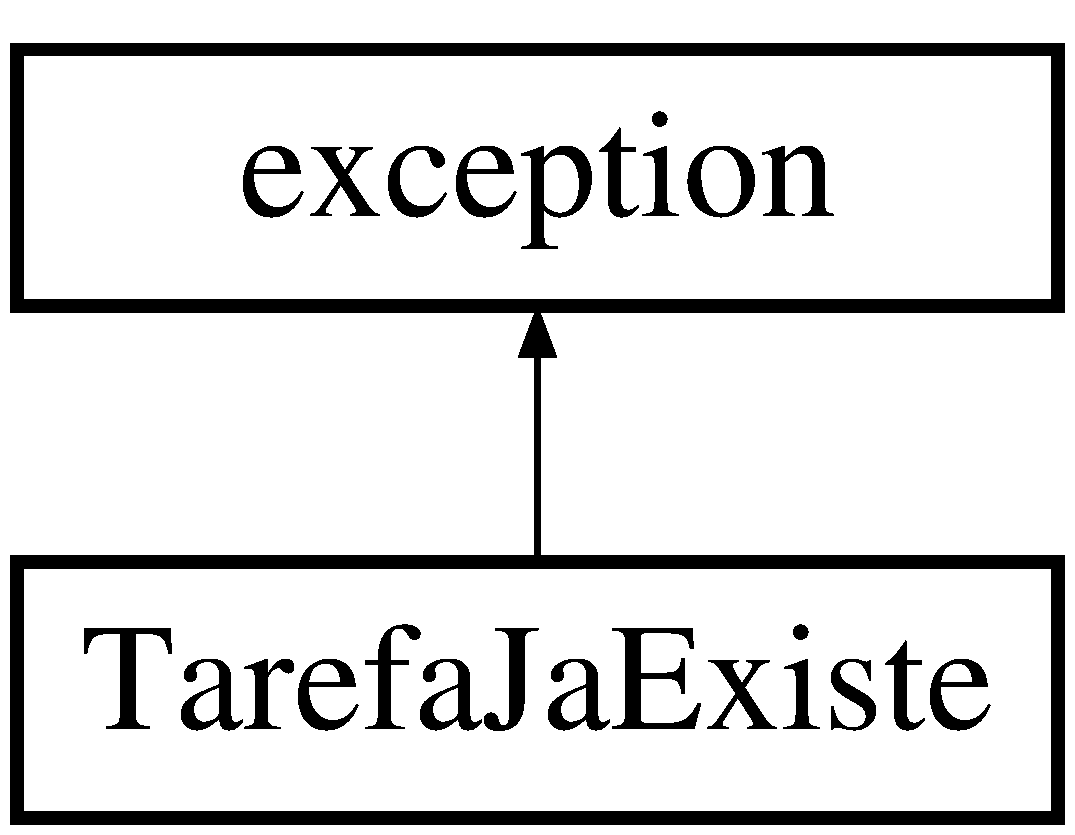
\includegraphics[height=2.000000cm]{classTarefaJaExiste}
\end{center}
\end{figure}
\subsection*{Public Member Functions}
\begin{DoxyCompactItemize}
\item 
const char $\ast$ \hyperlink{classTarefaJaExiste_a22f1eadc9e9c35239fc2bc529e3effc5}{what} () const noexcept override
\end{DoxyCompactItemize}
\subsection*{Private Attributes}
\begin{DoxyCompactItemize}
\item 
string \hyperlink{classTarefaJaExiste_a29db5b452baf0e27ee2fa9f14c683ed0}{mensagem} = \char`\"{}Já existe uma tarefa com esse título. Tente novamente\char`\"{}
\end{DoxyCompactItemize}


\subsection{Member Function Documentation}
\mbox{\Hypertarget{classTarefaJaExiste_a22f1eadc9e9c35239fc2bc529e3effc5}\label{classTarefaJaExiste_a22f1eadc9e9c35239fc2bc529e3effc5}} 
\index{Tarefa\+Ja\+Existe@{Tarefa\+Ja\+Existe}!what@{what}}
\index{what@{what}!Tarefa\+Ja\+Existe@{Tarefa\+Ja\+Existe}}
\subsubsection{\texorpdfstring{what()}{what()}}
{\footnotesize\ttfamily const char$\ast$ Tarefa\+Ja\+Existe\+::what (\begin{DoxyParamCaption}{ }\end{DoxyParamCaption}) const\hspace{0.3cm}{\ttfamily [inline]}, {\ttfamily [override]}, {\ttfamily [noexcept]}}



\subsection{Member Data Documentation}
\mbox{\Hypertarget{classTarefaJaExiste_a29db5b452baf0e27ee2fa9f14c683ed0}\label{classTarefaJaExiste_a29db5b452baf0e27ee2fa9f14c683ed0}} 
\index{Tarefa\+Ja\+Existe@{Tarefa\+Ja\+Existe}!mensagem@{mensagem}}
\index{mensagem@{mensagem}!Tarefa\+Ja\+Existe@{Tarefa\+Ja\+Existe}}
\subsubsection{\texorpdfstring{mensagem}{mensagem}}
{\footnotesize\ttfamily string Tarefa\+Ja\+Existe\+::mensagem = \char`\"{}Já existe uma tarefa com esse título. Tente novamente\char`\"{}\hspace{0.3cm}{\ttfamily [private]}}



The documentation for this class was generated from the following file\+:\begin{DoxyCompactItemize}
\item 
include/excecoes/\hyperlink{exc__tarefa_8hpp}{exc\+\_\+tarefa.\+hpp}\end{DoxyCompactItemize}

\hypertarget{classTerminal}{}\section{Terminal Class Reference}
\label{classTerminal}\index{Terminal@{Terminal}}


{\ttfamily \#include $<$terminal.\+hpp$>$}

\subsection*{Public Member Functions}
\begin{DoxyCompactItemize}
\item 
\hyperlink{classTerminal_aa448509b5aa1ece53c3d86385655be0e}{Terminal} ()
\item 
bool \hyperlink{classTerminal_aed7124f0bc24d4b77971f16d2f186a9b}{print} (string msg, bool quebra\+\_\+de\+\_\+linha)
\item 
bool \hyperlink{classTerminal_ac93c6cd6c16b785783ad21ff7bf80ef6}{print\+\_\+sucesso} (string msg\+\_\+sucesso)
\item 
bool \hyperlink{classTerminal_af5e724ead0f64b07a48d87a9942997e8}{print\+\_\+erro} (string msg\+\_\+erro)
\item 
bool \hyperlink{classTerminal_ab0f81f0dd06888554d817481140c953d}{print\+\_\+centralizado} (string texto)
\item 
bool \hyperlink{classTerminal_a9bb92733eb900a01a88c4e2eee17d938}{print\+\_\+direita} (string texto)
\item 
bool \hyperlink{classTerminal_a7aa126267c7e71ed99082884610496c9}{limpa\+\_\+terminal} ()
\item 
string \hyperlink{classTerminal_af3b082b98755b9f60f02315e5d207538}{espaco\+\_\+vertical} ()
\item 
string \hyperlink{classTerminal_a74aa95517ba338132e791a2aefb77b7a}{espaco\+\_\+horizontal} ()
\item 
string \hyperlink{classTerminal_a55827d690f15a0b401d6ee01ae710020}{get\+\_\+entrada} ()
\item 
bool \hyperlink{classTerminal_a46650fa9443239037a1a75afd963e51b}{login\+\_\+ou\+\_\+registre} ()
\item 
bool \hyperlink{classTerminal_a7c4d6a98c2ae96474e6745ce0c18d459}{cria\+\_\+usuario} ()
\item 
bool \hyperlink{classTerminal_a83ec130f3b19df9b382d99484669a509}{faz\+\_\+login} ()
\item 
bool \hyperlink{classTerminal_af5853d7279661f75d23fb44ade174da2}{tem\+\_\+tarefas} ()
\item 
int \hyperlink{classTerminal_a32ee131eb01ec417804965d183699f78}{get\+\_\+qtd\+\_\+paginas} ()
\item 
int \hyperlink{classTerminal_a4e72c12f3a0e6e3028cd0a87253966ca}{get\+\_\+qtd\+\_\+paginas\+\_\+grupos} ()
\item 
int \hyperlink{classTerminal_a0ebaf26f7d680bcd1412c3c692c3b7b2}{get\+\_\+qtd\+\_\+paginas\+\_\+prd} ()
\item 
bool \hyperlink{classTerminal_ad61f4e49e2c7aad146ae193920c8e2e8}{print\+\_\+ajuda} ()
\item 
bool \hyperlink{classTerminal_a4b1699a246eedcad0762c074c27ed3dc}{print\+\_\+paginacao} (int pagina\+\_\+atual)
\item 
bool \hyperlink{classTerminal_a33b9112ee605314c941413afd3d045fc}{print\+\_\+paginacao\+\_\+grupos} (int pagina\+\_\+atual)
\item 
bool \hyperlink{classTerminal_af7c7bbdbe5c28a4e797a42b4247ff121}{print\+\_\+paginacao\+\_\+prd} (int pagina\+\_\+atual)
\item 
bool \hyperlink{classTerminal_ab077ac695729b722e0c0e07f8508aa55}{print\+\_\+cabecalho} ()
\item 
bool \hyperlink{classTerminal_ae90c7487c329e9210234456f4e2723d9}{print\+\_\+cabecalho\+\_\+grupo} ()
\item 
bool \hyperlink{classTerminal_aeb95c3c6aa25ee2fa7898ed144ab47b5}{print\+\_\+cabecalho\+\_\+prd} ()
\item 
bool \hyperlink{classTerminal_a661628dafc3f0227f4acb58c32c5090c}{pagina\+\_\+existe} (int pagina)
\item 
bool \hyperlink{classTerminal_af95bd1d7646ccffb64be117d5d16d4e5}{pagina\+\_\+grupo\+\_\+existe} (int pagina)
\item 
bool \hyperlink{classTerminal_a6ff33aa1b1b2a2120542cac16f81c4b5}{pagina\+\_\+prd\+\_\+existe} (int pagina)
\item 
bool \hyperlink{classTerminal_a3633af9ee180a1a129f9c33c1a3aa3b9}{print\+\_\+tarefa} (\hyperlink{classTarefa}{Tarefa} $\ast$tarefa, int id)
\item 
bool \hyperlink{classTerminal_a99b5e852d3339543af8d740422c0f58b}{print\+\_\+tarefas} (int pagina)
\item 
bool \hyperlink{classTerminal_af2b2089477ced07e4acf9e8acafcd2f4}{exibe\+\_\+tarefa} (string comando)
\item 
bool \hyperlink{classTerminal_ae0951f8966234d5ec902112368a7c4a8}{print\+\_\+grupo} (\hyperlink{classGrupo}{Grupo} $\ast$grupo, int id)
\item 
bool \hyperlink{classTerminal_a1b8493b5a3ad18fe1f0ee784a70c6d77}{print\+\_\+grupos} (int pagina)
\item 
bool \hyperlink{classTerminal_a1065a9f3083675e569a9ea49a07e5036}{print\+\_\+prioridade} (\hyperlink{classPrioridade}{Prioridade} $\ast$prioridade, int id)
\item 
bool \hyperlink{classTerminal_a2c636ad455aa6e8f4ee0fc57be74fb09}{print\+\_\+prioridades} (int pagina)
\item 
bool \hyperlink{classTerminal_a04c02a475ddfd34ab7ac354ef35b8878}{prazo\+\_\+valido} (string prazo)
\item 
bool \hyperlink{classTerminal_a05c347f323568a234ea3e12bc0c64315}{nova\+\_\+tarefa} ()
\item 
bool \hyperlink{classTerminal_a80591e4cc7da1010d922a4ffca469eba}{novo\+\_\+grupo} ()
\item 
bool \hyperlink{classTerminal_a15369b06a58cb3b06bfac023e21a2e6e}{nova\+\_\+prioridade} ()
\item 
bool \hyperlink{classTerminal_ae01a6f6ca1a48721d6327051e6fe6a22}{editar\+\_\+titulo\+\_\+tarefa} (string comando)
\item 
bool \hyperlink{classTerminal_a1700bd13d74d5b81ff870bfccfc20e86}{editar\+\_\+desc\+\_\+tarefa} (string comando)
\item 
bool \hyperlink{classTerminal_ae0ddc1e5b294f6fbe62a5a70c267cb72}{editar\+\_\+prazo\+\_\+tarefa} (string comando)
\item 
bool \hyperlink{classTerminal_a08b680a0760ae5fbab03fa2098250c7b}{editar\+\_\+grupo\+\_\+tarefa} (string comando)
\item 
bool \hyperlink{classTerminal_abeeb442470656d2b6a4bf90079c35d74}{editar\+\_\+prd\+\_\+tarefa} (string comando)
\item 
bool \hyperlink{classTerminal_a63b9f303409fd5e787b7918b3d462e51}{marcar\+\_\+concluida} (string comando)
\item 
bool \hyperlink{classTerminal_aad539ca6e1d50e024ec4256bdf3b0e00}{desmarcar\+\_\+concluida} (string comando)
\item 
bool \hyperlink{classTerminal_a542446375398d23c429e38ce92ef2855}{editar\+\_\+nome\+\_\+grupo} (string comando)
\item 
bool \hyperlink{classTerminal_a318e04ea1bea16073451b6014fcde53e}{editar\+\_\+desc\+\_\+grupo} (string comando)
\item 
bool \hyperlink{classTerminal_a2d1957dcc0e404c16073f9c15fa2508e}{editar\+\_\+nome\+\_\+prd} (string comando)
\item 
bool \hyperlink{classTerminal_ad8941034607b656e5dcd279ce35a3f54}{editar\+\_\+nivel\+\_\+prd} (string comando)
\item 
bool \hyperlink{classTerminal_a207ca524c3b42aeb03d8e4aca1eee4a0}{deletar\+\_\+tarefa} (string comando)
\item 
bool \hyperlink{classTerminal_a915f2d35fcd5452b57af7af9af496c1e}{deletar\+\_\+grupo} (string comando)
\item 
bool \hyperlink{classTerminal_ac3e557f2c92b1f3a28e7a1363cd002a5}{deletar\+\_\+prioridade} (string comando)
\item 
void \hyperlink{classTerminal_ab5fabe06475207244e238a860e2aa469}{logout} ()
\item 
bool \hyperlink{classTerminal_a7447fa08bbace168d7e3043d13ad3fa4}{pede\+\_\+comando} ()
\item 
bool \hyperlink{classTerminal_aae5f31b6a4f5f1d7e7dcbbb438408fb4}{inicia} ()
\end{DoxyCompactItemize}
\subsection*{Private Attributes}
\begin{DoxyCompactItemize}
\item 
int \hyperlink{classTerminal_ac8f19b80b3c009efad6017cf5236510a}{\+\_\+largura\+\_\+terminal}
\item 
int \hyperlink{classTerminal_ac23f70e4a6bfe74cb430d10ce14f7d69}{\+\_\+altura\+\_\+terminal}
\item 
int \hyperlink{classTerminal_aa11effca90a9379eeee9776a41a79456}{\+\_\+padding\+\_\+y}
\item 
int \hyperlink{classTerminal_ac50acd9b920ff6d6759f953527869ea0}{\+\_\+padding\+\_\+x}
\item 
unsigned int \hyperlink{classTerminal_a51ad09d06d4ca9f3204d266d94c8fdcc}{\+\_\+tarefas\+\_\+por\+\_\+pagina}
\item 
\hyperlink{classUsuario}{Usuario} \hyperlink{classTerminal_aa5f996ee61173aaacf9b843fa211426e}{\+\_\+usuario}
\item 
\hyperlink{classStorage}{Storage} $\ast$ \hyperlink{classTerminal_a13bab737b1972d98bc4c8912fad52b2a}{\+\_\+storage}
\item 
unsigned int \hyperlink{classTerminal_ae16d3b2e118315e028a06cea51e1a5ac}{\+\_\+pagina\+\_\+atual}
\end{DoxyCompactItemize}


\subsection{Constructor \& Destructor Documentation}
\mbox{\Hypertarget{classTerminal_aa448509b5aa1ece53c3d86385655be0e}\label{classTerminal_aa448509b5aa1ece53c3d86385655be0e}} 
\index{Terminal@{Terminal}!Terminal@{Terminal}}
\index{Terminal@{Terminal}!Terminal@{Terminal}}
\subsubsection{\texorpdfstring{Terminal()}{Terminal()}}
{\footnotesize\ttfamily Terminal\+::\+Terminal (\begin{DoxyParamCaption}{ }\end{DoxyParamCaption})}



\subsection{Member Function Documentation}
\mbox{\Hypertarget{classTerminal_a7c4d6a98c2ae96474e6745ce0c18d459}\label{classTerminal_a7c4d6a98c2ae96474e6745ce0c18d459}} 
\index{Terminal@{Terminal}!cria\+\_\+usuario@{cria\+\_\+usuario}}
\index{cria\+\_\+usuario@{cria\+\_\+usuario}!Terminal@{Terminal}}
\subsubsection{\texorpdfstring{cria\+\_\+usuario()}{cria\_usuario()}}
{\footnotesize\ttfamily bool Terminal\+::cria\+\_\+usuario (\begin{DoxyParamCaption}{ }\end{DoxyParamCaption})}

\mbox{\Hypertarget{classTerminal_a915f2d35fcd5452b57af7af9af496c1e}\label{classTerminal_a915f2d35fcd5452b57af7af9af496c1e}} 
\index{Terminal@{Terminal}!deletar\+\_\+grupo@{deletar\+\_\+grupo}}
\index{deletar\+\_\+grupo@{deletar\+\_\+grupo}!Terminal@{Terminal}}
\subsubsection{\texorpdfstring{deletar\+\_\+grupo()}{deletar\_grupo()}}
{\footnotesize\ttfamily bool Terminal\+::deletar\+\_\+grupo (\begin{DoxyParamCaption}\item[{string}]{comando }\end{DoxyParamCaption})}

\mbox{\Hypertarget{classTerminal_ac3e557f2c92b1f3a28e7a1363cd002a5}\label{classTerminal_ac3e557f2c92b1f3a28e7a1363cd002a5}} 
\index{Terminal@{Terminal}!deletar\+\_\+prioridade@{deletar\+\_\+prioridade}}
\index{deletar\+\_\+prioridade@{deletar\+\_\+prioridade}!Terminal@{Terminal}}
\subsubsection{\texorpdfstring{deletar\+\_\+prioridade()}{deletar\_prioridade()}}
{\footnotesize\ttfamily bool Terminal\+::deletar\+\_\+prioridade (\begin{DoxyParamCaption}\item[{string}]{comando }\end{DoxyParamCaption})}

\mbox{\Hypertarget{classTerminal_a207ca524c3b42aeb03d8e4aca1eee4a0}\label{classTerminal_a207ca524c3b42aeb03d8e4aca1eee4a0}} 
\index{Terminal@{Terminal}!deletar\+\_\+tarefa@{deletar\+\_\+tarefa}}
\index{deletar\+\_\+tarefa@{deletar\+\_\+tarefa}!Terminal@{Terminal}}
\subsubsection{\texorpdfstring{deletar\+\_\+tarefa()}{deletar\_tarefa()}}
{\footnotesize\ttfamily bool Terminal\+::deletar\+\_\+tarefa (\begin{DoxyParamCaption}\item[{string}]{comando }\end{DoxyParamCaption})}

\mbox{\Hypertarget{classTerminal_aad539ca6e1d50e024ec4256bdf3b0e00}\label{classTerminal_aad539ca6e1d50e024ec4256bdf3b0e00}} 
\index{Terminal@{Terminal}!desmarcar\+\_\+concluida@{desmarcar\+\_\+concluida}}
\index{desmarcar\+\_\+concluida@{desmarcar\+\_\+concluida}!Terminal@{Terminal}}
\subsubsection{\texorpdfstring{desmarcar\+\_\+concluida()}{desmarcar\_concluida()}}
{\footnotesize\ttfamily bool Terminal\+::desmarcar\+\_\+concluida (\begin{DoxyParamCaption}\item[{string}]{comando }\end{DoxyParamCaption})}

\mbox{\Hypertarget{classTerminal_a318e04ea1bea16073451b6014fcde53e}\label{classTerminal_a318e04ea1bea16073451b6014fcde53e}} 
\index{Terminal@{Terminal}!editar\+\_\+desc\+\_\+grupo@{editar\+\_\+desc\+\_\+grupo}}
\index{editar\+\_\+desc\+\_\+grupo@{editar\+\_\+desc\+\_\+grupo}!Terminal@{Terminal}}
\subsubsection{\texorpdfstring{editar\+\_\+desc\+\_\+grupo()}{editar\_desc\_grupo()}}
{\footnotesize\ttfamily bool Terminal\+::editar\+\_\+desc\+\_\+grupo (\begin{DoxyParamCaption}\item[{string}]{comando }\end{DoxyParamCaption})}

\mbox{\Hypertarget{classTerminal_a1700bd13d74d5b81ff870bfccfc20e86}\label{classTerminal_a1700bd13d74d5b81ff870bfccfc20e86}} 
\index{Terminal@{Terminal}!editar\+\_\+desc\+\_\+tarefa@{editar\+\_\+desc\+\_\+tarefa}}
\index{editar\+\_\+desc\+\_\+tarefa@{editar\+\_\+desc\+\_\+tarefa}!Terminal@{Terminal}}
\subsubsection{\texorpdfstring{editar\+\_\+desc\+\_\+tarefa()}{editar\_desc\_tarefa()}}
{\footnotesize\ttfamily bool Terminal\+::editar\+\_\+desc\+\_\+tarefa (\begin{DoxyParamCaption}\item[{string}]{comando }\end{DoxyParamCaption})}

\mbox{\Hypertarget{classTerminal_a08b680a0760ae5fbab03fa2098250c7b}\label{classTerminal_a08b680a0760ae5fbab03fa2098250c7b}} 
\index{Terminal@{Terminal}!editar\+\_\+grupo\+\_\+tarefa@{editar\+\_\+grupo\+\_\+tarefa}}
\index{editar\+\_\+grupo\+\_\+tarefa@{editar\+\_\+grupo\+\_\+tarefa}!Terminal@{Terminal}}
\subsubsection{\texorpdfstring{editar\+\_\+grupo\+\_\+tarefa()}{editar\_grupo\_tarefa()}}
{\footnotesize\ttfamily bool Terminal\+::editar\+\_\+grupo\+\_\+tarefa (\begin{DoxyParamCaption}\item[{string}]{comando }\end{DoxyParamCaption})}

\mbox{\Hypertarget{classTerminal_ad8941034607b656e5dcd279ce35a3f54}\label{classTerminal_ad8941034607b656e5dcd279ce35a3f54}} 
\index{Terminal@{Terminal}!editar\+\_\+nivel\+\_\+prd@{editar\+\_\+nivel\+\_\+prd}}
\index{editar\+\_\+nivel\+\_\+prd@{editar\+\_\+nivel\+\_\+prd}!Terminal@{Terminal}}
\subsubsection{\texorpdfstring{editar\+\_\+nivel\+\_\+prd()}{editar\_nivel\_prd()}}
{\footnotesize\ttfamily bool Terminal\+::editar\+\_\+nivel\+\_\+prd (\begin{DoxyParamCaption}\item[{string}]{comando }\end{DoxyParamCaption})}

\mbox{\Hypertarget{classTerminal_a542446375398d23c429e38ce92ef2855}\label{classTerminal_a542446375398d23c429e38ce92ef2855}} 
\index{Terminal@{Terminal}!editar\+\_\+nome\+\_\+grupo@{editar\+\_\+nome\+\_\+grupo}}
\index{editar\+\_\+nome\+\_\+grupo@{editar\+\_\+nome\+\_\+grupo}!Terminal@{Terminal}}
\subsubsection{\texorpdfstring{editar\+\_\+nome\+\_\+grupo()}{editar\_nome\_grupo()}}
{\footnotesize\ttfamily bool Terminal\+::editar\+\_\+nome\+\_\+grupo (\begin{DoxyParamCaption}\item[{string}]{comando }\end{DoxyParamCaption})}

\mbox{\Hypertarget{classTerminal_a2d1957dcc0e404c16073f9c15fa2508e}\label{classTerminal_a2d1957dcc0e404c16073f9c15fa2508e}} 
\index{Terminal@{Terminal}!editar\+\_\+nome\+\_\+prd@{editar\+\_\+nome\+\_\+prd}}
\index{editar\+\_\+nome\+\_\+prd@{editar\+\_\+nome\+\_\+prd}!Terminal@{Terminal}}
\subsubsection{\texorpdfstring{editar\+\_\+nome\+\_\+prd()}{editar\_nome\_prd()}}
{\footnotesize\ttfamily bool Terminal\+::editar\+\_\+nome\+\_\+prd (\begin{DoxyParamCaption}\item[{string}]{comando }\end{DoxyParamCaption})}

\mbox{\Hypertarget{classTerminal_ae0ddc1e5b294f6fbe62a5a70c267cb72}\label{classTerminal_ae0ddc1e5b294f6fbe62a5a70c267cb72}} 
\index{Terminal@{Terminal}!editar\+\_\+prazo\+\_\+tarefa@{editar\+\_\+prazo\+\_\+tarefa}}
\index{editar\+\_\+prazo\+\_\+tarefa@{editar\+\_\+prazo\+\_\+tarefa}!Terminal@{Terminal}}
\subsubsection{\texorpdfstring{editar\+\_\+prazo\+\_\+tarefa()}{editar\_prazo\_tarefa()}}
{\footnotesize\ttfamily bool Terminal\+::editar\+\_\+prazo\+\_\+tarefa (\begin{DoxyParamCaption}\item[{string}]{comando }\end{DoxyParamCaption})}

\mbox{\Hypertarget{classTerminal_abeeb442470656d2b6a4bf90079c35d74}\label{classTerminal_abeeb442470656d2b6a4bf90079c35d74}} 
\index{Terminal@{Terminal}!editar\+\_\+prd\+\_\+tarefa@{editar\+\_\+prd\+\_\+tarefa}}
\index{editar\+\_\+prd\+\_\+tarefa@{editar\+\_\+prd\+\_\+tarefa}!Terminal@{Terminal}}
\subsubsection{\texorpdfstring{editar\+\_\+prd\+\_\+tarefa()}{editar\_prd\_tarefa()}}
{\footnotesize\ttfamily bool Terminal\+::editar\+\_\+prd\+\_\+tarefa (\begin{DoxyParamCaption}\item[{string}]{comando }\end{DoxyParamCaption})}

\mbox{\Hypertarget{classTerminal_ae01a6f6ca1a48721d6327051e6fe6a22}\label{classTerminal_ae01a6f6ca1a48721d6327051e6fe6a22}} 
\index{Terminal@{Terminal}!editar\+\_\+titulo\+\_\+tarefa@{editar\+\_\+titulo\+\_\+tarefa}}
\index{editar\+\_\+titulo\+\_\+tarefa@{editar\+\_\+titulo\+\_\+tarefa}!Terminal@{Terminal}}
\subsubsection{\texorpdfstring{editar\+\_\+titulo\+\_\+tarefa()}{editar\_titulo\_tarefa()}}
{\footnotesize\ttfamily bool Terminal\+::editar\+\_\+titulo\+\_\+tarefa (\begin{DoxyParamCaption}\item[{string}]{comando }\end{DoxyParamCaption})}

\mbox{\Hypertarget{classTerminal_a74aa95517ba338132e791a2aefb77b7a}\label{classTerminal_a74aa95517ba338132e791a2aefb77b7a}} 
\index{Terminal@{Terminal}!espaco\+\_\+horizontal@{espaco\+\_\+horizontal}}
\index{espaco\+\_\+horizontal@{espaco\+\_\+horizontal}!Terminal@{Terminal}}
\subsubsection{\texorpdfstring{espaco\+\_\+horizontal()}{espaco\_horizontal()}}
{\footnotesize\ttfamily string Terminal\+::espaco\+\_\+horizontal (\begin{DoxyParamCaption}{ }\end{DoxyParamCaption})}

\mbox{\Hypertarget{classTerminal_af3b082b98755b9f60f02315e5d207538}\label{classTerminal_af3b082b98755b9f60f02315e5d207538}} 
\index{Terminal@{Terminal}!espaco\+\_\+vertical@{espaco\+\_\+vertical}}
\index{espaco\+\_\+vertical@{espaco\+\_\+vertical}!Terminal@{Terminal}}
\subsubsection{\texorpdfstring{espaco\+\_\+vertical()}{espaco\_vertical()}}
{\footnotesize\ttfamily string Terminal\+::espaco\+\_\+vertical (\begin{DoxyParamCaption}{ }\end{DoxyParamCaption})}

\mbox{\Hypertarget{classTerminal_af2b2089477ced07e4acf9e8acafcd2f4}\label{classTerminal_af2b2089477ced07e4acf9e8acafcd2f4}} 
\index{Terminal@{Terminal}!exibe\+\_\+tarefa@{exibe\+\_\+tarefa}}
\index{exibe\+\_\+tarefa@{exibe\+\_\+tarefa}!Terminal@{Terminal}}
\subsubsection{\texorpdfstring{exibe\+\_\+tarefa()}{exibe\_tarefa()}}
{\footnotesize\ttfamily bool Terminal\+::exibe\+\_\+tarefa (\begin{DoxyParamCaption}\item[{string}]{comando }\end{DoxyParamCaption})}

\mbox{\Hypertarget{classTerminal_a83ec130f3b19df9b382d99484669a509}\label{classTerminal_a83ec130f3b19df9b382d99484669a509}} 
\index{Terminal@{Terminal}!faz\+\_\+login@{faz\+\_\+login}}
\index{faz\+\_\+login@{faz\+\_\+login}!Terminal@{Terminal}}
\subsubsection{\texorpdfstring{faz\+\_\+login()}{faz\_login()}}
{\footnotesize\ttfamily bool Terminal\+::faz\+\_\+login (\begin{DoxyParamCaption}{ }\end{DoxyParamCaption})}

\mbox{\Hypertarget{classTerminal_a55827d690f15a0b401d6ee01ae710020}\label{classTerminal_a55827d690f15a0b401d6ee01ae710020}} 
\index{Terminal@{Terminal}!get\+\_\+entrada@{get\+\_\+entrada}}
\index{get\+\_\+entrada@{get\+\_\+entrada}!Terminal@{Terminal}}
\subsubsection{\texorpdfstring{get\+\_\+entrada()}{get\_entrada()}}
{\footnotesize\ttfamily string Terminal\+::get\+\_\+entrada (\begin{DoxyParamCaption}{ }\end{DoxyParamCaption})}

\mbox{\Hypertarget{classTerminal_a32ee131eb01ec417804965d183699f78}\label{classTerminal_a32ee131eb01ec417804965d183699f78}} 
\index{Terminal@{Terminal}!get\+\_\+qtd\+\_\+paginas@{get\+\_\+qtd\+\_\+paginas}}
\index{get\+\_\+qtd\+\_\+paginas@{get\+\_\+qtd\+\_\+paginas}!Terminal@{Terminal}}
\subsubsection{\texorpdfstring{get\+\_\+qtd\+\_\+paginas()}{get\_qtd\_paginas()}}
{\footnotesize\ttfamily int Terminal\+::get\+\_\+qtd\+\_\+paginas (\begin{DoxyParamCaption}{ }\end{DoxyParamCaption})}

\mbox{\Hypertarget{classTerminal_a4e72c12f3a0e6e3028cd0a87253966ca}\label{classTerminal_a4e72c12f3a0e6e3028cd0a87253966ca}} 
\index{Terminal@{Terminal}!get\+\_\+qtd\+\_\+paginas\+\_\+grupos@{get\+\_\+qtd\+\_\+paginas\+\_\+grupos}}
\index{get\+\_\+qtd\+\_\+paginas\+\_\+grupos@{get\+\_\+qtd\+\_\+paginas\+\_\+grupos}!Terminal@{Terminal}}
\subsubsection{\texorpdfstring{get\+\_\+qtd\+\_\+paginas\+\_\+grupos()}{get\_qtd\_paginas\_grupos()}}
{\footnotesize\ttfamily int Terminal\+::get\+\_\+qtd\+\_\+paginas\+\_\+grupos (\begin{DoxyParamCaption}{ }\end{DoxyParamCaption})}

\mbox{\Hypertarget{classTerminal_a0ebaf26f7d680bcd1412c3c692c3b7b2}\label{classTerminal_a0ebaf26f7d680bcd1412c3c692c3b7b2}} 
\index{Terminal@{Terminal}!get\+\_\+qtd\+\_\+paginas\+\_\+prd@{get\+\_\+qtd\+\_\+paginas\+\_\+prd}}
\index{get\+\_\+qtd\+\_\+paginas\+\_\+prd@{get\+\_\+qtd\+\_\+paginas\+\_\+prd}!Terminal@{Terminal}}
\subsubsection{\texorpdfstring{get\+\_\+qtd\+\_\+paginas\+\_\+prd()}{get\_qtd\_paginas\_prd()}}
{\footnotesize\ttfamily int Terminal\+::get\+\_\+qtd\+\_\+paginas\+\_\+prd (\begin{DoxyParamCaption}{ }\end{DoxyParamCaption})}

\mbox{\Hypertarget{classTerminal_aae5f31b6a4f5f1d7e7dcbbb438408fb4}\label{classTerminal_aae5f31b6a4f5f1d7e7dcbbb438408fb4}} 
\index{Terminal@{Terminal}!inicia@{inicia}}
\index{inicia@{inicia}!Terminal@{Terminal}}
\subsubsection{\texorpdfstring{inicia()}{inicia()}}
{\footnotesize\ttfamily bool Terminal\+::inicia (\begin{DoxyParamCaption}{ }\end{DoxyParamCaption})}

\mbox{\Hypertarget{classTerminal_a7aa126267c7e71ed99082884610496c9}\label{classTerminal_a7aa126267c7e71ed99082884610496c9}} 
\index{Terminal@{Terminal}!limpa\+\_\+terminal@{limpa\+\_\+terminal}}
\index{limpa\+\_\+terminal@{limpa\+\_\+terminal}!Terminal@{Terminal}}
\subsubsection{\texorpdfstring{limpa\+\_\+terminal()}{limpa\_terminal()}}
{\footnotesize\ttfamily bool Terminal\+::limpa\+\_\+terminal (\begin{DoxyParamCaption}{ }\end{DoxyParamCaption})}

\mbox{\Hypertarget{classTerminal_a46650fa9443239037a1a75afd963e51b}\label{classTerminal_a46650fa9443239037a1a75afd963e51b}} 
\index{Terminal@{Terminal}!login\+\_\+ou\+\_\+registre@{login\+\_\+ou\+\_\+registre}}
\index{login\+\_\+ou\+\_\+registre@{login\+\_\+ou\+\_\+registre}!Terminal@{Terminal}}
\subsubsection{\texorpdfstring{login\+\_\+ou\+\_\+registre()}{login\_ou\_registre()}}
{\footnotesize\ttfamily bool Terminal\+::login\+\_\+ou\+\_\+registre (\begin{DoxyParamCaption}{ }\end{DoxyParamCaption})}

\mbox{\Hypertarget{classTerminal_ab5fabe06475207244e238a860e2aa469}\label{classTerminal_ab5fabe06475207244e238a860e2aa469}} 
\index{Terminal@{Terminal}!logout@{logout}}
\index{logout@{logout}!Terminal@{Terminal}}
\subsubsection{\texorpdfstring{logout()}{logout()}}
{\footnotesize\ttfamily void Terminal\+::logout (\begin{DoxyParamCaption}{ }\end{DoxyParamCaption})}

\mbox{\Hypertarget{classTerminal_a63b9f303409fd5e787b7918b3d462e51}\label{classTerminal_a63b9f303409fd5e787b7918b3d462e51}} 
\index{Terminal@{Terminal}!marcar\+\_\+concluida@{marcar\+\_\+concluida}}
\index{marcar\+\_\+concluida@{marcar\+\_\+concluida}!Terminal@{Terminal}}
\subsubsection{\texorpdfstring{marcar\+\_\+concluida()}{marcar\_concluida()}}
{\footnotesize\ttfamily bool Terminal\+::marcar\+\_\+concluida (\begin{DoxyParamCaption}\item[{string}]{comando }\end{DoxyParamCaption})}

\mbox{\Hypertarget{classTerminal_a15369b06a58cb3b06bfac023e21a2e6e}\label{classTerminal_a15369b06a58cb3b06bfac023e21a2e6e}} 
\index{Terminal@{Terminal}!nova\+\_\+prioridade@{nova\+\_\+prioridade}}
\index{nova\+\_\+prioridade@{nova\+\_\+prioridade}!Terminal@{Terminal}}
\subsubsection{\texorpdfstring{nova\+\_\+prioridade()}{nova\_prioridade()}}
{\footnotesize\ttfamily bool Terminal\+::nova\+\_\+prioridade (\begin{DoxyParamCaption}{ }\end{DoxyParamCaption})}

\mbox{\Hypertarget{classTerminal_a05c347f323568a234ea3e12bc0c64315}\label{classTerminal_a05c347f323568a234ea3e12bc0c64315}} 
\index{Terminal@{Terminal}!nova\+\_\+tarefa@{nova\+\_\+tarefa}}
\index{nova\+\_\+tarefa@{nova\+\_\+tarefa}!Terminal@{Terminal}}
\subsubsection{\texorpdfstring{nova\+\_\+tarefa()}{nova\_tarefa()}}
{\footnotesize\ttfamily bool Terminal\+::nova\+\_\+tarefa (\begin{DoxyParamCaption}{ }\end{DoxyParamCaption})}

\mbox{\Hypertarget{classTerminal_a80591e4cc7da1010d922a4ffca469eba}\label{classTerminal_a80591e4cc7da1010d922a4ffca469eba}} 
\index{Terminal@{Terminal}!novo\+\_\+grupo@{novo\+\_\+grupo}}
\index{novo\+\_\+grupo@{novo\+\_\+grupo}!Terminal@{Terminal}}
\subsubsection{\texorpdfstring{novo\+\_\+grupo()}{novo\_grupo()}}
{\footnotesize\ttfamily bool Terminal\+::novo\+\_\+grupo (\begin{DoxyParamCaption}{ }\end{DoxyParamCaption})}

\mbox{\Hypertarget{classTerminal_a661628dafc3f0227f4acb58c32c5090c}\label{classTerminal_a661628dafc3f0227f4acb58c32c5090c}} 
\index{Terminal@{Terminal}!pagina\+\_\+existe@{pagina\+\_\+existe}}
\index{pagina\+\_\+existe@{pagina\+\_\+existe}!Terminal@{Terminal}}
\subsubsection{\texorpdfstring{pagina\+\_\+existe()}{pagina\_existe()}}
{\footnotesize\ttfamily bool Terminal\+::pagina\+\_\+existe (\begin{DoxyParamCaption}\item[{int}]{pagina }\end{DoxyParamCaption})}

\mbox{\Hypertarget{classTerminal_af95bd1d7646ccffb64be117d5d16d4e5}\label{classTerminal_af95bd1d7646ccffb64be117d5d16d4e5}} 
\index{Terminal@{Terminal}!pagina\+\_\+grupo\+\_\+existe@{pagina\+\_\+grupo\+\_\+existe}}
\index{pagina\+\_\+grupo\+\_\+existe@{pagina\+\_\+grupo\+\_\+existe}!Terminal@{Terminal}}
\subsubsection{\texorpdfstring{pagina\+\_\+grupo\+\_\+existe()}{pagina\_grupo\_existe()}}
{\footnotesize\ttfamily bool Terminal\+::pagina\+\_\+grupo\+\_\+existe (\begin{DoxyParamCaption}\item[{int}]{pagina }\end{DoxyParamCaption})}

\mbox{\Hypertarget{classTerminal_a6ff33aa1b1b2a2120542cac16f81c4b5}\label{classTerminal_a6ff33aa1b1b2a2120542cac16f81c4b5}} 
\index{Terminal@{Terminal}!pagina\+\_\+prd\+\_\+existe@{pagina\+\_\+prd\+\_\+existe}}
\index{pagina\+\_\+prd\+\_\+existe@{pagina\+\_\+prd\+\_\+existe}!Terminal@{Terminal}}
\subsubsection{\texorpdfstring{pagina\+\_\+prd\+\_\+existe()}{pagina\_prd\_existe()}}
{\footnotesize\ttfamily bool Terminal\+::pagina\+\_\+prd\+\_\+existe (\begin{DoxyParamCaption}\item[{int}]{pagina }\end{DoxyParamCaption})}

\mbox{\Hypertarget{classTerminal_a7447fa08bbace168d7e3043d13ad3fa4}\label{classTerminal_a7447fa08bbace168d7e3043d13ad3fa4}} 
\index{Terminal@{Terminal}!pede\+\_\+comando@{pede\+\_\+comando}}
\index{pede\+\_\+comando@{pede\+\_\+comando}!Terminal@{Terminal}}
\subsubsection{\texorpdfstring{pede\+\_\+comando()}{pede\_comando()}}
{\footnotesize\ttfamily bool Terminal\+::pede\+\_\+comando (\begin{DoxyParamCaption}{ }\end{DoxyParamCaption})}

\mbox{\Hypertarget{classTerminal_a04c02a475ddfd34ab7ac354ef35b8878}\label{classTerminal_a04c02a475ddfd34ab7ac354ef35b8878}} 
\index{Terminal@{Terminal}!prazo\+\_\+valido@{prazo\+\_\+valido}}
\index{prazo\+\_\+valido@{prazo\+\_\+valido}!Terminal@{Terminal}}
\subsubsection{\texorpdfstring{prazo\+\_\+valido()}{prazo\_valido()}}
{\footnotesize\ttfamily bool Terminal\+::prazo\+\_\+valido (\begin{DoxyParamCaption}\item[{string}]{prazo }\end{DoxyParamCaption})}

\mbox{\Hypertarget{classTerminal_aed7124f0bc24d4b77971f16d2f186a9b}\label{classTerminal_aed7124f0bc24d4b77971f16d2f186a9b}} 
\index{Terminal@{Terminal}!print@{print}}
\index{print@{print}!Terminal@{Terminal}}
\subsubsection{\texorpdfstring{print()}{print()}}
{\footnotesize\ttfamily bool Terminal\+::print (\begin{DoxyParamCaption}\item[{string}]{msg,  }\item[{bool}]{quebra\+\_\+de\+\_\+linha }\end{DoxyParamCaption})}

\mbox{\Hypertarget{classTerminal_ad61f4e49e2c7aad146ae193920c8e2e8}\label{classTerminal_ad61f4e49e2c7aad146ae193920c8e2e8}} 
\index{Terminal@{Terminal}!print\+\_\+ajuda@{print\+\_\+ajuda}}
\index{print\+\_\+ajuda@{print\+\_\+ajuda}!Terminal@{Terminal}}
\subsubsection{\texorpdfstring{print\+\_\+ajuda()}{print\_ajuda()}}
{\footnotesize\ttfamily bool Terminal\+::print\+\_\+ajuda (\begin{DoxyParamCaption}{ }\end{DoxyParamCaption})}

\mbox{\Hypertarget{classTerminal_ab077ac695729b722e0c0e07f8508aa55}\label{classTerminal_ab077ac695729b722e0c0e07f8508aa55}} 
\index{Terminal@{Terminal}!print\+\_\+cabecalho@{print\+\_\+cabecalho}}
\index{print\+\_\+cabecalho@{print\+\_\+cabecalho}!Terminal@{Terminal}}
\subsubsection{\texorpdfstring{print\+\_\+cabecalho()}{print\_cabecalho()}}
{\footnotesize\ttfamily bool Terminal\+::print\+\_\+cabecalho (\begin{DoxyParamCaption}{ }\end{DoxyParamCaption})}

\mbox{\Hypertarget{classTerminal_ae90c7487c329e9210234456f4e2723d9}\label{classTerminal_ae90c7487c329e9210234456f4e2723d9}} 
\index{Terminal@{Terminal}!print\+\_\+cabecalho\+\_\+grupo@{print\+\_\+cabecalho\+\_\+grupo}}
\index{print\+\_\+cabecalho\+\_\+grupo@{print\+\_\+cabecalho\+\_\+grupo}!Terminal@{Terminal}}
\subsubsection{\texorpdfstring{print\+\_\+cabecalho\+\_\+grupo()}{print\_cabecalho\_grupo()}}
{\footnotesize\ttfamily bool Terminal\+::print\+\_\+cabecalho\+\_\+grupo (\begin{DoxyParamCaption}{ }\end{DoxyParamCaption})}

\mbox{\Hypertarget{classTerminal_aeb95c3c6aa25ee2fa7898ed144ab47b5}\label{classTerminal_aeb95c3c6aa25ee2fa7898ed144ab47b5}} 
\index{Terminal@{Terminal}!print\+\_\+cabecalho\+\_\+prd@{print\+\_\+cabecalho\+\_\+prd}}
\index{print\+\_\+cabecalho\+\_\+prd@{print\+\_\+cabecalho\+\_\+prd}!Terminal@{Terminal}}
\subsubsection{\texorpdfstring{print\+\_\+cabecalho\+\_\+prd()}{print\_cabecalho\_prd()}}
{\footnotesize\ttfamily bool Terminal\+::print\+\_\+cabecalho\+\_\+prd (\begin{DoxyParamCaption}{ }\end{DoxyParamCaption})}

\mbox{\Hypertarget{classTerminal_ab0f81f0dd06888554d817481140c953d}\label{classTerminal_ab0f81f0dd06888554d817481140c953d}} 
\index{Terminal@{Terminal}!print\+\_\+centralizado@{print\+\_\+centralizado}}
\index{print\+\_\+centralizado@{print\+\_\+centralizado}!Terminal@{Terminal}}
\subsubsection{\texorpdfstring{print\+\_\+centralizado()}{print\_centralizado()}}
{\footnotesize\ttfamily bool Terminal\+::print\+\_\+centralizado (\begin{DoxyParamCaption}\item[{string}]{texto }\end{DoxyParamCaption})}

\mbox{\Hypertarget{classTerminal_a9bb92733eb900a01a88c4e2eee17d938}\label{classTerminal_a9bb92733eb900a01a88c4e2eee17d938}} 
\index{Terminal@{Terminal}!print\+\_\+direita@{print\+\_\+direita}}
\index{print\+\_\+direita@{print\+\_\+direita}!Terminal@{Terminal}}
\subsubsection{\texorpdfstring{print\+\_\+direita()}{print\_direita()}}
{\footnotesize\ttfamily bool Terminal\+::print\+\_\+direita (\begin{DoxyParamCaption}\item[{string}]{texto }\end{DoxyParamCaption})}

\mbox{\Hypertarget{classTerminal_af5e724ead0f64b07a48d87a9942997e8}\label{classTerminal_af5e724ead0f64b07a48d87a9942997e8}} 
\index{Terminal@{Terminal}!print\+\_\+erro@{print\+\_\+erro}}
\index{print\+\_\+erro@{print\+\_\+erro}!Terminal@{Terminal}}
\subsubsection{\texorpdfstring{print\+\_\+erro()}{print\_erro()}}
{\footnotesize\ttfamily bool Terminal\+::print\+\_\+erro (\begin{DoxyParamCaption}\item[{string}]{msg\+\_\+erro }\end{DoxyParamCaption})}

\mbox{\Hypertarget{classTerminal_ae0951f8966234d5ec902112368a7c4a8}\label{classTerminal_ae0951f8966234d5ec902112368a7c4a8}} 
\index{Terminal@{Terminal}!print\+\_\+grupo@{print\+\_\+grupo}}
\index{print\+\_\+grupo@{print\+\_\+grupo}!Terminal@{Terminal}}
\subsubsection{\texorpdfstring{print\+\_\+grupo()}{print\_grupo()}}
{\footnotesize\ttfamily bool Terminal\+::print\+\_\+grupo (\begin{DoxyParamCaption}\item[{\hyperlink{classGrupo}{Grupo} $\ast$}]{grupo,  }\item[{int}]{id }\end{DoxyParamCaption})}

\mbox{\Hypertarget{classTerminal_a1b8493b5a3ad18fe1f0ee784a70c6d77}\label{classTerminal_a1b8493b5a3ad18fe1f0ee784a70c6d77}} 
\index{Terminal@{Terminal}!print\+\_\+grupos@{print\+\_\+grupos}}
\index{print\+\_\+grupos@{print\+\_\+grupos}!Terminal@{Terminal}}
\subsubsection{\texorpdfstring{print\+\_\+grupos()}{print\_grupos()}}
{\footnotesize\ttfamily bool Terminal\+::print\+\_\+grupos (\begin{DoxyParamCaption}\item[{int}]{pagina }\end{DoxyParamCaption})}

\mbox{\Hypertarget{classTerminal_a4b1699a246eedcad0762c074c27ed3dc}\label{classTerminal_a4b1699a246eedcad0762c074c27ed3dc}} 
\index{Terminal@{Terminal}!print\+\_\+paginacao@{print\+\_\+paginacao}}
\index{print\+\_\+paginacao@{print\+\_\+paginacao}!Terminal@{Terminal}}
\subsubsection{\texorpdfstring{print\+\_\+paginacao()}{print\_paginacao()}}
{\footnotesize\ttfamily bool Terminal\+::print\+\_\+paginacao (\begin{DoxyParamCaption}\item[{int}]{pagina\+\_\+atual }\end{DoxyParamCaption})}

\mbox{\Hypertarget{classTerminal_a33b9112ee605314c941413afd3d045fc}\label{classTerminal_a33b9112ee605314c941413afd3d045fc}} 
\index{Terminal@{Terminal}!print\+\_\+paginacao\+\_\+grupos@{print\+\_\+paginacao\+\_\+grupos}}
\index{print\+\_\+paginacao\+\_\+grupos@{print\+\_\+paginacao\+\_\+grupos}!Terminal@{Terminal}}
\subsubsection{\texorpdfstring{print\+\_\+paginacao\+\_\+grupos()}{print\_paginacao\_grupos()}}
{\footnotesize\ttfamily bool Terminal\+::print\+\_\+paginacao\+\_\+grupos (\begin{DoxyParamCaption}\item[{int}]{pagina\+\_\+atual }\end{DoxyParamCaption})}

\mbox{\Hypertarget{classTerminal_af7c7bbdbe5c28a4e797a42b4247ff121}\label{classTerminal_af7c7bbdbe5c28a4e797a42b4247ff121}} 
\index{Terminal@{Terminal}!print\+\_\+paginacao\+\_\+prd@{print\+\_\+paginacao\+\_\+prd}}
\index{print\+\_\+paginacao\+\_\+prd@{print\+\_\+paginacao\+\_\+prd}!Terminal@{Terminal}}
\subsubsection{\texorpdfstring{print\+\_\+paginacao\+\_\+prd()}{print\_paginacao\_prd()}}
{\footnotesize\ttfamily bool Terminal\+::print\+\_\+paginacao\+\_\+prd (\begin{DoxyParamCaption}\item[{int}]{pagina\+\_\+atual }\end{DoxyParamCaption})}

\mbox{\Hypertarget{classTerminal_a1065a9f3083675e569a9ea49a07e5036}\label{classTerminal_a1065a9f3083675e569a9ea49a07e5036}} 
\index{Terminal@{Terminal}!print\+\_\+prioridade@{print\+\_\+prioridade}}
\index{print\+\_\+prioridade@{print\+\_\+prioridade}!Terminal@{Terminal}}
\subsubsection{\texorpdfstring{print\+\_\+prioridade()}{print\_prioridade()}}
{\footnotesize\ttfamily bool Terminal\+::print\+\_\+prioridade (\begin{DoxyParamCaption}\item[{\hyperlink{classPrioridade}{Prioridade} $\ast$}]{prioridade,  }\item[{int}]{id }\end{DoxyParamCaption})}

\mbox{\Hypertarget{classTerminal_a2c636ad455aa6e8f4ee0fc57be74fb09}\label{classTerminal_a2c636ad455aa6e8f4ee0fc57be74fb09}} 
\index{Terminal@{Terminal}!print\+\_\+prioridades@{print\+\_\+prioridades}}
\index{print\+\_\+prioridades@{print\+\_\+prioridades}!Terminal@{Terminal}}
\subsubsection{\texorpdfstring{print\+\_\+prioridades()}{print\_prioridades()}}
{\footnotesize\ttfamily bool Terminal\+::print\+\_\+prioridades (\begin{DoxyParamCaption}\item[{int}]{pagina }\end{DoxyParamCaption})}

\mbox{\Hypertarget{classTerminal_ac93c6cd6c16b785783ad21ff7bf80ef6}\label{classTerminal_ac93c6cd6c16b785783ad21ff7bf80ef6}} 
\index{Terminal@{Terminal}!print\+\_\+sucesso@{print\+\_\+sucesso}}
\index{print\+\_\+sucesso@{print\+\_\+sucesso}!Terminal@{Terminal}}
\subsubsection{\texorpdfstring{print\+\_\+sucesso()}{print\_sucesso()}}
{\footnotesize\ttfamily bool Terminal\+::print\+\_\+sucesso (\begin{DoxyParamCaption}\item[{string}]{msg\+\_\+sucesso }\end{DoxyParamCaption})}

\mbox{\Hypertarget{classTerminal_a3633af9ee180a1a129f9c33c1a3aa3b9}\label{classTerminal_a3633af9ee180a1a129f9c33c1a3aa3b9}} 
\index{Terminal@{Terminal}!print\+\_\+tarefa@{print\+\_\+tarefa}}
\index{print\+\_\+tarefa@{print\+\_\+tarefa}!Terminal@{Terminal}}
\subsubsection{\texorpdfstring{print\+\_\+tarefa()}{print\_tarefa()}}
{\footnotesize\ttfamily bool Terminal\+::print\+\_\+tarefa (\begin{DoxyParamCaption}\item[{\hyperlink{classTarefa}{Tarefa} $\ast$}]{tarefa,  }\item[{int}]{id }\end{DoxyParamCaption})}

\mbox{\Hypertarget{classTerminal_a99b5e852d3339543af8d740422c0f58b}\label{classTerminal_a99b5e852d3339543af8d740422c0f58b}} 
\index{Terminal@{Terminal}!print\+\_\+tarefas@{print\+\_\+tarefas}}
\index{print\+\_\+tarefas@{print\+\_\+tarefas}!Terminal@{Terminal}}
\subsubsection{\texorpdfstring{print\+\_\+tarefas()}{print\_tarefas()}}
{\footnotesize\ttfamily bool Terminal\+::print\+\_\+tarefas (\begin{DoxyParamCaption}\item[{int}]{pagina }\end{DoxyParamCaption})}

\mbox{\Hypertarget{classTerminal_af5853d7279661f75d23fb44ade174da2}\label{classTerminal_af5853d7279661f75d23fb44ade174da2}} 
\index{Terminal@{Terminal}!tem\+\_\+tarefas@{tem\+\_\+tarefas}}
\index{tem\+\_\+tarefas@{tem\+\_\+tarefas}!Terminal@{Terminal}}
\subsubsection{\texorpdfstring{tem\+\_\+tarefas()}{tem\_tarefas()}}
{\footnotesize\ttfamily bool Terminal\+::tem\+\_\+tarefas (\begin{DoxyParamCaption}{ }\end{DoxyParamCaption})}



\subsection{Member Data Documentation}
\mbox{\Hypertarget{classTerminal_ac23f70e4a6bfe74cb430d10ce14f7d69}\label{classTerminal_ac23f70e4a6bfe74cb430d10ce14f7d69}} 
\index{Terminal@{Terminal}!\+\_\+altura\+\_\+terminal@{\+\_\+altura\+\_\+terminal}}
\index{\+\_\+altura\+\_\+terminal@{\+\_\+altura\+\_\+terminal}!Terminal@{Terminal}}
\subsubsection{\texorpdfstring{\+\_\+altura\+\_\+terminal}{\_altura\_terminal}}
{\footnotesize\ttfamily int Terminal\+::\+\_\+altura\+\_\+terminal\hspace{0.3cm}{\ttfamily [private]}}

\mbox{\Hypertarget{classTerminal_ac8f19b80b3c009efad6017cf5236510a}\label{classTerminal_ac8f19b80b3c009efad6017cf5236510a}} 
\index{Terminal@{Terminal}!\+\_\+largura\+\_\+terminal@{\+\_\+largura\+\_\+terminal}}
\index{\+\_\+largura\+\_\+terminal@{\+\_\+largura\+\_\+terminal}!Terminal@{Terminal}}
\subsubsection{\texorpdfstring{\+\_\+largura\+\_\+terminal}{\_largura\_terminal}}
{\footnotesize\ttfamily int Terminal\+::\+\_\+largura\+\_\+terminal\hspace{0.3cm}{\ttfamily [private]}}

\mbox{\Hypertarget{classTerminal_ac50acd9b920ff6d6759f953527869ea0}\label{classTerminal_ac50acd9b920ff6d6759f953527869ea0}} 
\index{Terminal@{Terminal}!\+\_\+padding\+\_\+x@{\+\_\+padding\+\_\+x}}
\index{\+\_\+padding\+\_\+x@{\+\_\+padding\+\_\+x}!Terminal@{Terminal}}
\subsubsection{\texorpdfstring{\+\_\+padding\+\_\+x}{\_padding\_x}}
{\footnotesize\ttfamily int Terminal\+::\+\_\+padding\+\_\+x\hspace{0.3cm}{\ttfamily [private]}}

\mbox{\Hypertarget{classTerminal_aa11effca90a9379eeee9776a41a79456}\label{classTerminal_aa11effca90a9379eeee9776a41a79456}} 
\index{Terminal@{Terminal}!\+\_\+padding\+\_\+y@{\+\_\+padding\+\_\+y}}
\index{\+\_\+padding\+\_\+y@{\+\_\+padding\+\_\+y}!Terminal@{Terminal}}
\subsubsection{\texorpdfstring{\+\_\+padding\+\_\+y}{\_padding\_y}}
{\footnotesize\ttfamily int Terminal\+::\+\_\+padding\+\_\+y\hspace{0.3cm}{\ttfamily [private]}}

\mbox{\Hypertarget{classTerminal_ae16d3b2e118315e028a06cea51e1a5ac}\label{classTerminal_ae16d3b2e118315e028a06cea51e1a5ac}} 
\index{Terminal@{Terminal}!\+\_\+pagina\+\_\+atual@{\+\_\+pagina\+\_\+atual}}
\index{\+\_\+pagina\+\_\+atual@{\+\_\+pagina\+\_\+atual}!Terminal@{Terminal}}
\subsubsection{\texorpdfstring{\+\_\+pagina\+\_\+atual}{\_pagina\_atual}}
{\footnotesize\ttfamily unsigned int Terminal\+::\+\_\+pagina\+\_\+atual\hspace{0.3cm}{\ttfamily [private]}}

\mbox{\Hypertarget{classTerminal_a13bab737b1972d98bc4c8912fad52b2a}\label{classTerminal_a13bab737b1972d98bc4c8912fad52b2a}} 
\index{Terminal@{Terminal}!\+\_\+storage@{\+\_\+storage}}
\index{\+\_\+storage@{\+\_\+storage}!Terminal@{Terminal}}
\subsubsection{\texorpdfstring{\+\_\+storage}{\_storage}}
{\footnotesize\ttfamily \hyperlink{classStorage}{Storage}$\ast$ Terminal\+::\+\_\+storage\hspace{0.3cm}{\ttfamily [private]}}

\mbox{\Hypertarget{classTerminal_a51ad09d06d4ca9f3204d266d94c8fdcc}\label{classTerminal_a51ad09d06d4ca9f3204d266d94c8fdcc}} 
\index{Terminal@{Terminal}!\+\_\+tarefas\+\_\+por\+\_\+pagina@{\+\_\+tarefas\+\_\+por\+\_\+pagina}}
\index{\+\_\+tarefas\+\_\+por\+\_\+pagina@{\+\_\+tarefas\+\_\+por\+\_\+pagina}!Terminal@{Terminal}}
\subsubsection{\texorpdfstring{\+\_\+tarefas\+\_\+por\+\_\+pagina}{\_tarefas\_por\_pagina}}
{\footnotesize\ttfamily unsigned int Terminal\+::\+\_\+tarefas\+\_\+por\+\_\+pagina\hspace{0.3cm}{\ttfamily [private]}}

\mbox{\Hypertarget{classTerminal_aa5f996ee61173aaacf9b843fa211426e}\label{classTerminal_aa5f996ee61173aaacf9b843fa211426e}} 
\index{Terminal@{Terminal}!\+\_\+usuario@{\+\_\+usuario}}
\index{\+\_\+usuario@{\+\_\+usuario}!Terminal@{Terminal}}
\subsubsection{\texorpdfstring{\+\_\+usuario}{\_usuario}}
{\footnotesize\ttfamily \hyperlink{classUsuario}{Usuario} Terminal\+::\+\_\+usuario\hspace{0.3cm}{\ttfamily [private]}}



The documentation for this class was generated from the following file\+:\begin{DoxyCompactItemize}
\item 
include/\hyperlink{terminal_8hpp}{terminal.\+hpp}\end{DoxyCompactItemize}

\hypertarget{classUsuario}{}\section{Usuario Class Reference}
\label{classUsuario}\index{Usuario@{Usuario}}


{\ttfamily \#include $<$usuario.\+hpp$>$}

\subsection*{Public Member Functions}
\begin{DoxyCompactItemize}
\item 
\hyperlink{classUsuario_aa85a5371a098dfba5449140d9b8a472f}{Usuario} ()
\item 
\hyperlink{classUsuario_a0cde516a7cd7901bd255c0d5552b67cb}{Usuario} (string usuario, string senha)
\item 
string \hyperlink{classUsuario_a65e8e43842bcaa429a4f971b2b950e2c}{get\+\_\+nome} ()
\item 
\hyperlink{classStorage}{Storage} $\ast$ \hyperlink{classUsuario_a29f0b4619fc682fdfa3f53c7488b3a33}{get\+\_\+storage} ()
\end{DoxyCompactItemize}
\subsection*{Private Attributes}
\begin{DoxyCompactItemize}
\item 
string \hyperlink{classUsuario_a1f8c614f94b3ac85915bf27aedd86ffb}{\+\_\+nome\+\_\+usuario}
\item 
\hyperlink{classStorage}{Storage} $\ast$ \hyperlink{classUsuario_ab513a33701fd16851c1307906913bf10}{\+\_\+storage}
\end{DoxyCompactItemize}


\subsection{Constructor \& Destructor Documentation}
\mbox{\Hypertarget{classUsuario_aa85a5371a098dfba5449140d9b8a472f}\label{classUsuario_aa85a5371a098dfba5449140d9b8a472f}} 
\index{Usuario@{Usuario}!Usuario@{Usuario}}
\index{Usuario@{Usuario}!Usuario@{Usuario}}
\subsubsection{\texorpdfstring{Usuario()}{Usuario()}\hspace{0.1cm}{\footnotesize\ttfamily [1/2]}}
{\footnotesize\ttfamily Usuario\+::\+Usuario (\begin{DoxyParamCaption}{ }\end{DoxyParamCaption})}

\mbox{\Hypertarget{classUsuario_a0cde516a7cd7901bd255c0d5552b67cb}\label{classUsuario_a0cde516a7cd7901bd255c0d5552b67cb}} 
\index{Usuario@{Usuario}!Usuario@{Usuario}}
\index{Usuario@{Usuario}!Usuario@{Usuario}}
\subsubsection{\texorpdfstring{Usuario()}{Usuario()}\hspace{0.1cm}{\footnotesize\ttfamily [2/2]}}
{\footnotesize\ttfamily Usuario\+::\+Usuario (\begin{DoxyParamCaption}\item[{string}]{usuario,  }\item[{string}]{senha }\end{DoxyParamCaption})}



\subsection{Member Function Documentation}
\mbox{\Hypertarget{classUsuario_a65e8e43842bcaa429a4f971b2b950e2c}\label{classUsuario_a65e8e43842bcaa429a4f971b2b950e2c}} 
\index{Usuario@{Usuario}!get\+\_\+nome@{get\+\_\+nome}}
\index{get\+\_\+nome@{get\+\_\+nome}!Usuario@{Usuario}}
\subsubsection{\texorpdfstring{get\+\_\+nome()}{get\_nome()}}
{\footnotesize\ttfamily string Usuario\+::get\+\_\+nome (\begin{DoxyParamCaption}{ }\end{DoxyParamCaption})}

\mbox{\Hypertarget{classUsuario_a29f0b4619fc682fdfa3f53c7488b3a33}\label{classUsuario_a29f0b4619fc682fdfa3f53c7488b3a33}} 
\index{Usuario@{Usuario}!get\+\_\+storage@{get\+\_\+storage}}
\index{get\+\_\+storage@{get\+\_\+storage}!Usuario@{Usuario}}
\subsubsection{\texorpdfstring{get\+\_\+storage()}{get\_storage()}}
{\footnotesize\ttfamily \hyperlink{classStorage}{Storage}$\ast$ Usuario\+::get\+\_\+storage (\begin{DoxyParamCaption}{ }\end{DoxyParamCaption})}



\subsection{Member Data Documentation}
\mbox{\Hypertarget{classUsuario_a1f8c614f94b3ac85915bf27aedd86ffb}\label{classUsuario_a1f8c614f94b3ac85915bf27aedd86ffb}} 
\index{Usuario@{Usuario}!\+\_\+nome\+\_\+usuario@{\+\_\+nome\+\_\+usuario}}
\index{\+\_\+nome\+\_\+usuario@{\+\_\+nome\+\_\+usuario}!Usuario@{Usuario}}
\subsubsection{\texorpdfstring{\+\_\+nome\+\_\+usuario}{\_nome\_usuario}}
{\footnotesize\ttfamily string Usuario\+::\+\_\+nome\+\_\+usuario\hspace{0.3cm}{\ttfamily [private]}}

\mbox{\Hypertarget{classUsuario_ab513a33701fd16851c1307906913bf10}\label{classUsuario_ab513a33701fd16851c1307906913bf10}} 
\index{Usuario@{Usuario}!\+\_\+storage@{\+\_\+storage}}
\index{\+\_\+storage@{\+\_\+storage}!Usuario@{Usuario}}
\subsubsection{\texorpdfstring{\+\_\+storage}{\_storage}}
{\footnotesize\ttfamily \hyperlink{classStorage}{Storage}$\ast$ Usuario\+::\+\_\+storage\hspace{0.3cm}{\ttfamily [private]}}



The documentation for this class was generated from the following file\+:\begin{DoxyCompactItemize}
\item 
include/\hyperlink{usuario_8hpp}{usuario.\+hpp}\end{DoxyCompactItemize}

\hypertarget{classUsuarioJaExiste}{}\section{Usuario\+Ja\+Existe Class Reference}
\label{classUsuarioJaExiste}\index{Usuario\+Ja\+Existe@{Usuario\+Ja\+Existe}}


{\ttfamily \#include $<$exc\+\_\+usuario.\+hpp$>$}

Inheritance diagram for Usuario\+Ja\+Existe\+:\begin{figure}[H]
\begin{center}
\leavevmode
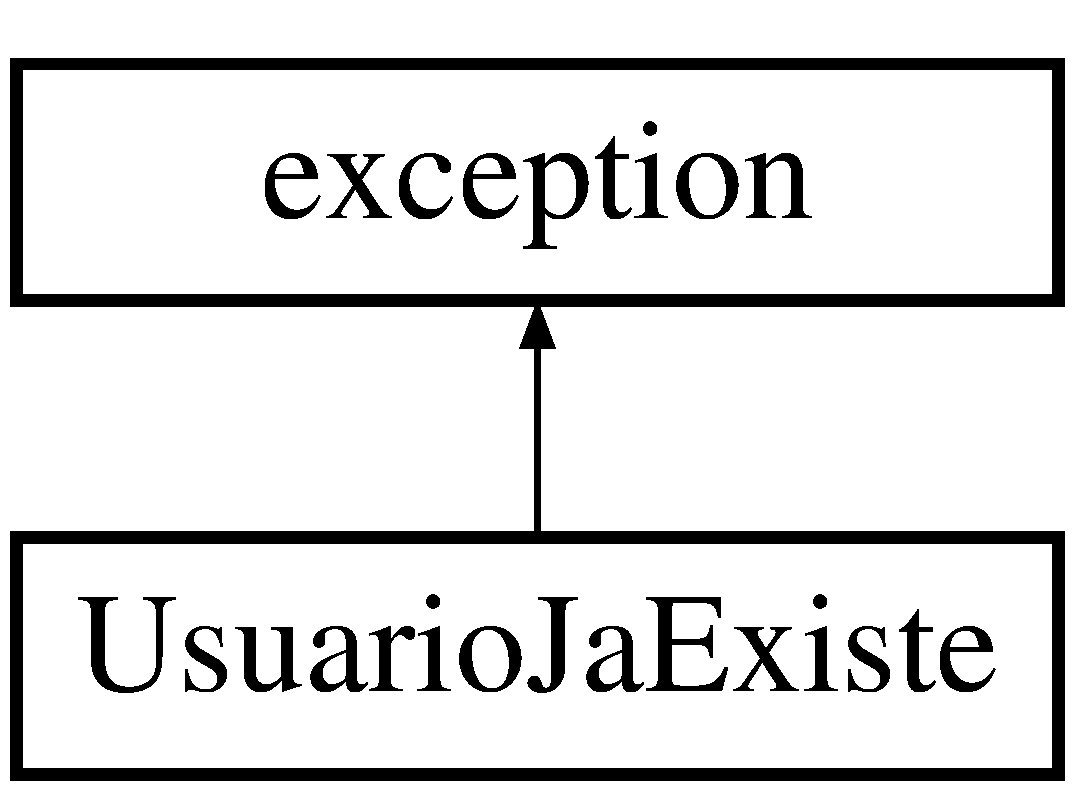
\includegraphics[height=2.000000cm]{classUsuarioJaExiste}
\end{center}
\end{figure}
\subsection*{Public Member Functions}
\begin{DoxyCompactItemize}
\item 
const char $\ast$ \hyperlink{classUsuarioJaExiste_abe722b380a1cb83ac87f350fbb5d5261}{what} () const noexcept override
\end{DoxyCompactItemize}
\subsection*{Private Attributes}
\begin{DoxyCompactItemize}
\item 
string \hyperlink{classUsuarioJaExiste_abd00539263f588798844b87f64eab9a7}{mensagem} = \char`\"{}Já existe um usuário com esse nome. Tente novamente.\char`\"{}
\end{DoxyCompactItemize}


\subsection{Member Function Documentation}
\mbox{\Hypertarget{classUsuarioJaExiste_abe722b380a1cb83ac87f350fbb5d5261}\label{classUsuarioJaExiste_abe722b380a1cb83ac87f350fbb5d5261}} 
\index{Usuario\+Ja\+Existe@{Usuario\+Ja\+Existe}!what@{what}}
\index{what@{what}!Usuario\+Ja\+Existe@{Usuario\+Ja\+Existe}}
\subsubsection{\texorpdfstring{what()}{what()}}
{\footnotesize\ttfamily const char$\ast$ Usuario\+Ja\+Existe\+::what (\begin{DoxyParamCaption}{ }\end{DoxyParamCaption}) const\hspace{0.3cm}{\ttfamily [inline]}, {\ttfamily [override]}, {\ttfamily [noexcept]}}



\subsection{Member Data Documentation}
\mbox{\Hypertarget{classUsuarioJaExiste_abd00539263f588798844b87f64eab9a7}\label{classUsuarioJaExiste_abd00539263f588798844b87f64eab9a7}} 
\index{Usuario\+Ja\+Existe@{Usuario\+Ja\+Existe}!mensagem@{mensagem}}
\index{mensagem@{mensagem}!Usuario\+Ja\+Existe@{Usuario\+Ja\+Existe}}
\subsubsection{\texorpdfstring{mensagem}{mensagem}}
{\footnotesize\ttfamily string Usuario\+Ja\+Existe\+::mensagem = \char`\"{}Já existe um usuário com esse nome. Tente novamente.\char`\"{}\hspace{0.3cm}{\ttfamily [private]}}



The documentation for this class was generated from the following file\+:\begin{DoxyCompactItemize}
\item 
include/excecoes/\hyperlink{exc__usuario_8hpp}{exc\+\_\+usuario.\+hpp}\end{DoxyCompactItemize}

\hypertarget{classUsuarioNaoEncontrado}{}\section{Usuario\+Nao\+Encontrado Class Reference}
\label{classUsuarioNaoEncontrado}\index{Usuario\+Nao\+Encontrado@{Usuario\+Nao\+Encontrado}}


{\ttfamily \#include $<$exc\+\_\+usuario.\+hpp$>$}

Inheritance diagram for Usuario\+Nao\+Encontrado\+:\begin{figure}[H]
\begin{center}
\leavevmode
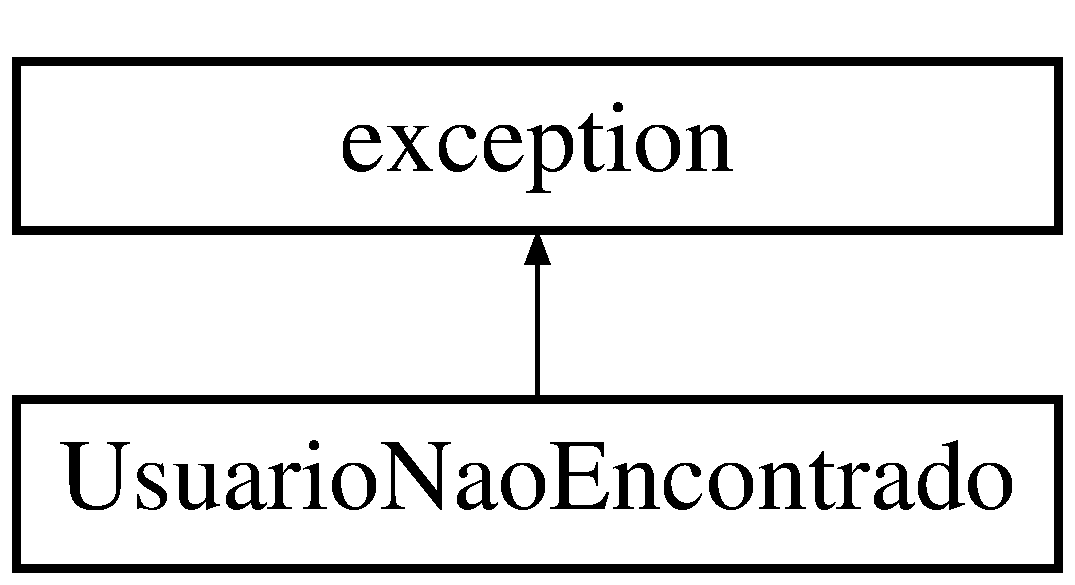
\includegraphics[height=2.000000cm]{classUsuarioNaoEncontrado}
\end{center}
\end{figure}
\subsection*{Public Member Functions}
\begin{DoxyCompactItemize}
\item 
const char $\ast$ \hyperlink{classUsuarioNaoEncontrado_a81dbc44d187226187e1fe4b81e6e816d}{what} () const noexcept override
\end{DoxyCompactItemize}
\subsection*{Private Attributes}
\begin{DoxyCompactItemize}
\item 
string \hyperlink{classUsuarioNaoEncontrado_abad07fdf50cec90997957a8282d29be4}{mensagem} = \char`\"{}Usuário não encontrado. Tente novamente.\char`\"{}
\end{DoxyCompactItemize}


\subsection{Member Function Documentation}
\mbox{\Hypertarget{classUsuarioNaoEncontrado_a81dbc44d187226187e1fe4b81e6e816d}\label{classUsuarioNaoEncontrado_a81dbc44d187226187e1fe4b81e6e816d}} 
\index{Usuario\+Nao\+Encontrado@{Usuario\+Nao\+Encontrado}!what@{what}}
\index{what@{what}!Usuario\+Nao\+Encontrado@{Usuario\+Nao\+Encontrado}}
\subsubsection{\texorpdfstring{what()}{what()}}
{\footnotesize\ttfamily const char$\ast$ Usuario\+Nao\+Encontrado\+::what (\begin{DoxyParamCaption}{ }\end{DoxyParamCaption}) const\hspace{0.3cm}{\ttfamily [inline]}, {\ttfamily [override]}, {\ttfamily [noexcept]}}



\subsection{Member Data Documentation}
\mbox{\Hypertarget{classUsuarioNaoEncontrado_abad07fdf50cec90997957a8282d29be4}\label{classUsuarioNaoEncontrado_abad07fdf50cec90997957a8282d29be4}} 
\index{Usuario\+Nao\+Encontrado@{Usuario\+Nao\+Encontrado}!mensagem@{mensagem}}
\index{mensagem@{mensagem}!Usuario\+Nao\+Encontrado@{Usuario\+Nao\+Encontrado}}
\subsubsection{\texorpdfstring{mensagem}{mensagem}}
{\footnotesize\ttfamily string Usuario\+Nao\+Encontrado\+::mensagem = \char`\"{}Usuário não encontrado. Tente novamente.\char`\"{}\hspace{0.3cm}{\ttfamily [private]}}



The documentation for this class was generated from the following file\+:\begin{DoxyCompactItemize}
\item 
include/excecoes/\hyperlink{exc__usuario_8hpp}{exc\+\_\+usuario.\+hpp}\end{DoxyCompactItemize}

\hypertarget{classValorPrioridadeInvalido}{}\section{Valor\+Prioridade\+Invalido Class Reference}
\label{classValorPrioridadeInvalido}\index{Valor\+Prioridade\+Invalido@{Valor\+Prioridade\+Invalido}}


{\ttfamily \#include $<$exc\+\_\+prioridade.\+hpp$>$}

Inheritance diagram for Valor\+Prioridade\+Invalido\+:\begin{figure}[H]
\begin{center}
\leavevmode
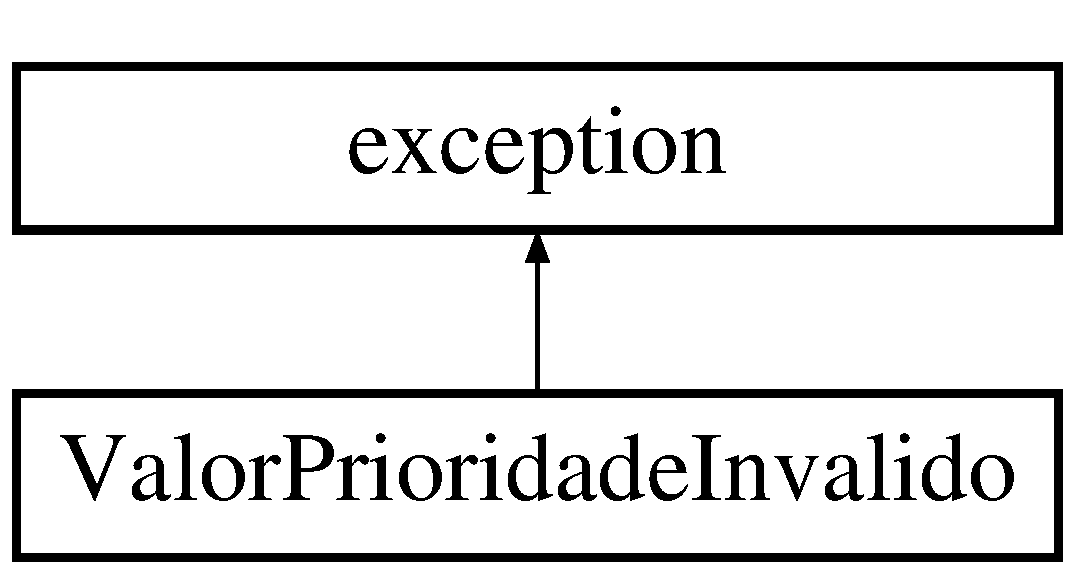
\includegraphics[height=2.000000cm]{classValorPrioridadeInvalido}
\end{center}
\end{figure}
\subsection*{Public Member Functions}
\begin{DoxyCompactItemize}
\item 
const char $\ast$ \hyperlink{classValorPrioridadeInvalido_a5cf2c87a65131e2e56848784c4dc77ea}{what} () const noexcept override
\end{DoxyCompactItemize}
\subsection*{Private Attributes}
\begin{DoxyCompactItemize}
\item 
string \hyperlink{classValorPrioridadeInvalido_af0cc68ad2ec7183808dc1a222a5cfa98}{mensagem} = \char`\"{}O valor da prioridade deve ser um número positivo. Tente novamente\char`\"{}
\end{DoxyCompactItemize}


\subsection{Member Function Documentation}
\mbox{\Hypertarget{classValorPrioridadeInvalido_a5cf2c87a65131e2e56848784c4dc77ea}\label{classValorPrioridadeInvalido_a5cf2c87a65131e2e56848784c4dc77ea}} 
\index{Valor\+Prioridade\+Invalido@{Valor\+Prioridade\+Invalido}!what@{what}}
\index{what@{what}!Valor\+Prioridade\+Invalido@{Valor\+Prioridade\+Invalido}}
\subsubsection{\texorpdfstring{what()}{what()}}
{\footnotesize\ttfamily const char$\ast$ Valor\+Prioridade\+Invalido\+::what (\begin{DoxyParamCaption}{ }\end{DoxyParamCaption}) const\hspace{0.3cm}{\ttfamily [inline]}, {\ttfamily [override]}, {\ttfamily [noexcept]}}



\subsection{Member Data Documentation}
\mbox{\Hypertarget{classValorPrioridadeInvalido_af0cc68ad2ec7183808dc1a222a5cfa98}\label{classValorPrioridadeInvalido_af0cc68ad2ec7183808dc1a222a5cfa98}} 
\index{Valor\+Prioridade\+Invalido@{Valor\+Prioridade\+Invalido}!mensagem@{mensagem}}
\index{mensagem@{mensagem}!Valor\+Prioridade\+Invalido@{Valor\+Prioridade\+Invalido}}
\subsubsection{\texorpdfstring{mensagem}{mensagem}}
{\footnotesize\ttfamily string Valor\+Prioridade\+Invalido\+::mensagem = \char`\"{}O valor da prioridade deve ser um número positivo. Tente novamente\char`\"{}\hspace{0.3cm}{\ttfamily [private]}}



The documentation for this class was generated from the following file\+:\begin{DoxyCompactItemize}
\item 
include/excecoes/\hyperlink{exc__prioridade_8hpp}{exc\+\_\+prioridade.\+hpp}\end{DoxyCompactItemize}

\chapter{File Documentation}
\hypertarget{etiqueta_8hpp}{}\section{include/etiqueta.hpp File Reference}
\label{etiqueta_8hpp}\index{include/etiqueta.\+hpp@{include/etiqueta.\+hpp}}
{\ttfamily \#include $<$string$>$}\newline
\subsection*{Classes}
\begin{DoxyCompactItemize}
\item 
class \hyperlink{classEtiqueta}{Etiqueta}
\end{DoxyCompactItemize}

\hypertarget{exc__arquivo_8hpp}{}\section{include/excecoes/exc\+\_\+arquivo.hpp File Reference}
\label{exc__arquivo_8hpp}\index{include/excecoes/exc\+\_\+arquivo.\+hpp@{include/excecoes/exc\+\_\+arquivo.\+hpp}}
{\ttfamily \#include $<$exception$>$}\newline
{\ttfamily \#include $<$string$>$}\newline
\subsection*{Classes}
\begin{DoxyCompactItemize}
\item 
class \hyperlink{classErroAoAbrirArquivo}{Erro\+Ao\+Abrir\+Arquivo}
\end{DoxyCompactItemize}

\hypertarget{exc__cancelamento_8hpp}{}\section{include/excecoes/exc\+\_\+cancelamento.hpp File Reference}
\label{exc__cancelamento_8hpp}\index{include/excecoes/exc\+\_\+cancelamento.\+hpp@{include/excecoes/exc\+\_\+cancelamento.\+hpp}}
{\ttfamily \#include $<$exception$>$}\newline
{\ttfamily \#include $<$string$>$}\newline
\subsection*{Classes}
\begin{DoxyCompactItemize}
\item 
class \hyperlink{classCriacaoTarefaCancelada}{Criacao\+Tarefa\+Cancelada}
\item 
class \hyperlink{classCriacaoGrupoCancelada}{Criacao\+Grupo\+Cancelada}
\item 
class \hyperlink{classCriacaoPrioridadeCancelada}{Criacao\+Prioridade\+Cancelada}
\item 
class \hyperlink{classEdicaoTarefaCancelada}{Edicao\+Tarefa\+Cancelada}
\item 
class \hyperlink{classEdicaoGrupoCancelada}{Edicao\+Grupo\+Cancelada}
\item 
class \hyperlink{classEdicaoPrioridadeCancelada}{Edicao\+Prioridade\+Cancelada}
\end{DoxyCompactItemize}

\hypertarget{exc__comando_8hpp}{}\section{include/excecoes/exc\+\_\+comando.hpp File Reference}
\label{exc__comando_8hpp}\index{include/excecoes/exc\+\_\+comando.\+hpp@{include/excecoes/exc\+\_\+comando.\+hpp}}
{\ttfamily \#include $<$exception$>$}\newline
{\ttfamily \#include $<$string$>$}\newline
\subsection*{Classes}
\begin{DoxyCompactItemize}
\item 
class \hyperlink{classComandoEditarTarefaErrado}{Comando\+Editar\+Tarefa\+Errado}
\item 
class \hyperlink{classComandoExcluirTarefaErrado}{Comando\+Excluir\+Tarefa\+Errado}
\item 
class \hyperlink{classComandoExibirTarefaErrado}{Comando\+Exibir\+Tarefa\+Errado}
\item 
class \hyperlink{classComandoEditarGrupoErrado}{Comando\+Editar\+Grupo\+Errado}
\item 
class \hyperlink{classComandoExcluirGrupoErrado}{Comando\+Excluir\+Grupo\+Errado}
\item 
class \hyperlink{classComandoEditarPrioridadeErrado}{Comando\+Editar\+Prioridade\+Errado}
\item 
class \hyperlink{classComandoExcluirPrioridadeErrado}{Comando\+Excluir\+Prioridade\+Errado}
\end{DoxyCompactItemize}

\hypertarget{exc__grupo_8hpp}{}\section{include/excecoes/exc\+\_\+grupo.hpp File Reference}
\label{exc__grupo_8hpp}\index{include/excecoes/exc\+\_\+grupo.\+hpp@{include/excecoes/exc\+\_\+grupo.\+hpp}}
{\ttfamily \#include $<$exception$>$}\newline
{\ttfamily \#include $<$string$>$}\newline
\subsection*{Classes}
\begin{DoxyCompactItemize}
\item 
class \hyperlink{classNomeGrupoMuitoLongo}{Nome\+Grupo\+Muito\+Longo}
\item 
class \hyperlink{classIdGrupoNaoExiste}{Id\+Grupo\+Nao\+Existe}
\item 
class \hyperlink{classGrupoNaoExiste}{Grupo\+Nao\+Existe}
\item 
class \hyperlink{classGrupoJaExiste}{Grupo\+Ja\+Existe}
\item 
class \hyperlink{classErroAoApagarGrupo}{Erro\+Ao\+Apagar\+Grupo}
\end{DoxyCompactItemize}

\hypertarget{exc__pagina_8hpp}{}\section{include/excecoes/exc\+\_\+pagina.hpp File Reference}
\label{exc__pagina_8hpp}\index{include/excecoes/exc\+\_\+pagina.\+hpp@{include/excecoes/exc\+\_\+pagina.\+hpp}}
{\ttfamily \#include $<$exception$>$}\newline
{\ttfamily \#include $<$string$>$}\newline
\subsection*{Classes}
\begin{DoxyCompactItemize}
\item 
class \hyperlink{classPaginaInvalida}{Pagina\+Invalida}
\item 
class \hyperlink{classPaginaNaoInformada}{Pagina\+Nao\+Informada}
\end{DoxyCompactItemize}

\hypertarget{exc__prioridade_8hpp}{}\section{include/excecoes/exc\+\_\+prioridade.hpp File Reference}
\label{exc__prioridade_8hpp}\index{include/excecoes/exc\+\_\+prioridade.\+hpp@{include/excecoes/exc\+\_\+prioridade.\+hpp}}
{\ttfamily \#include $<$exception$>$}\newline
{\ttfamily \#include $<$string$>$}\newline
\subsection*{Classes}
\begin{DoxyCompactItemize}
\item 
class \hyperlink{classNomePrioridadeMuitoLongo}{Nome\+Prioridade\+Muito\+Longo}
\item 
class \hyperlink{classPrioridadeJaExiste}{Prioridade\+Ja\+Existe}
\item 
class \hyperlink{classValorPrioridadeInvalido}{Valor\+Prioridade\+Invalido}
\item 
class \hyperlink{classPrioridadeNaoExiste}{Prioridade\+Nao\+Existe}
\item 
class \hyperlink{classIdPrioridadeNaoExiste}{Id\+Prioridade\+Nao\+Existe}
\item 
class \hyperlink{classErroAoApagarPrioridade}{Erro\+Ao\+Apagar\+Prioridade}
\end{DoxyCompactItemize}

\hypertarget{exc__tarefa_8hpp}{}\section{include/excecoes/exc\+\_\+tarefa.hpp File Reference}
\label{exc__tarefa_8hpp}\index{include/excecoes/exc\+\_\+tarefa.\+hpp@{include/excecoes/exc\+\_\+tarefa.\+hpp}}
{\ttfamily \#include $<$exception$>$}\newline
{\ttfamily \#include $<$string$>$}\newline
\subsection*{Classes}
\begin{DoxyCompactItemize}
\item 
class \hyperlink{classNomeTarefaMuitoLongo}{Nome\+Tarefa\+Muito\+Longo}
\item 
class \hyperlink{classIdTarefaNaoExiste}{Id\+Tarefa\+Nao\+Existe}
\item 
class \hyperlink{classPrazoInvalido}{Prazo\+Invalido}
\item 
class \hyperlink{classTarefaJaExiste}{Tarefa\+Ja\+Existe}
\end{DoxyCompactItemize}

\hypertarget{exc__usuario_8hpp}{}\section{include/excecoes/exc\+\_\+usuario.hpp File Reference}
\label{exc__usuario_8hpp}\index{include/excecoes/exc\+\_\+usuario.\+hpp@{include/excecoes/exc\+\_\+usuario.\+hpp}}
{\ttfamily \#include $<$exception$>$}\newline
{\ttfamily \#include $<$string$>$}\newline
\subsection*{Classes}
\begin{DoxyCompactItemize}
\item 
class \hyperlink{classCaractereInvalido}{Caractere\+Invalido}
\item 
class \hyperlink{classUsuarioJaExiste}{Usuario\+Ja\+Existe}
\item 
class \hyperlink{classUsuarioNaoEncontrado}{Usuario\+Nao\+Encontrado}
\item 
class \hyperlink{classSenhaIncorreta}{Senha\+Incorreta}
\end{DoxyCompactItemize}

\hypertarget{file__util_8hpp}{}\section{include/file\+\_\+util.hpp File Reference}
\label{file__util_8hpp}\index{include/file\+\_\+util.\+hpp@{include/file\+\_\+util.\+hpp}}
{\ttfamily \#include $<$sys/stat.\+h$>$}\newline
{\ttfamily \#include $<$string$>$}\newline
{\ttfamily \#include $<$fstream$>$}\newline
\subsection*{Classes}
\begin{DoxyCompactItemize}
\item 
class \hyperlink{classFileUtil}{File\+Util}
\end{DoxyCompactItemize}

\hypertarget{grupo_8hpp}{}\section{include/grupo.hpp File Reference}
\label{grupo_8hpp}\index{include/grupo.\+hpp@{include/grupo.\+hpp}}
{\ttfamily \#include $<$string$>$}\newline
{\ttfamily \#include \char`\"{}etiqueta.\+hpp\char`\"{}}\newline
\subsection*{Classes}
\begin{DoxyCompactItemize}
\item 
class \hyperlink{classGrupo}{Grupo}
\end{DoxyCompactItemize}

\hypertarget{prioridade_8hpp}{}\section{include/prioridade.hpp File Reference}
\label{prioridade_8hpp}\index{include/prioridade.\+hpp@{include/prioridade.\+hpp}}
{\ttfamily \#include \char`\"{}etiqueta.\+hpp\char`\"{}}\newline
{\ttfamily \#include $<$string$>$}\newline
\subsection*{Classes}
\begin{DoxyCompactItemize}
\item 
class \hyperlink{classPrioridade}{Prioridade}
\end{DoxyCompactItemize}

\hypertarget{storage_8hpp}{}\section{include/storage.hpp File Reference}
\label{storage_8hpp}\index{include/storage.\+hpp@{include/storage.\+hpp}}
{\ttfamily \#include $<$fstream$>$}\newline
{\ttfamily \#include \char`\"{}etiqueta.\+hpp\char`\"{}}\newline
{\ttfamily \#include \char`\"{}grupo.\+hpp\char`\"{}}\newline
{\ttfamily \#include \char`\"{}string\char`\"{}}\newline
{\ttfamily \#include \char`\"{}file\+\_\+util.\+hpp\char`\"{}}\newline
{\ttfamily \#include \char`\"{}tarefa.\+hpp\char`\"{}}\newline
{\ttfamily \#include \char`\"{}prioridade.\+hpp\char`\"{}}\newline
{\ttfamily \#include \char`\"{}excecoes/exc\+\_\+usuario.\+hpp\char`\"{}}\newline
{\ttfamily \#include \char`\"{}excecoes/exc\+\_\+grupo.\+hpp\char`\"{}}\newline
{\ttfamily \#include \char`\"{}excecoes/exc\+\_\+prioridade.\+hpp\char`\"{}}\newline
{\ttfamily \#include \char`\"{}excecoes/exc\+\_\+arquivo.\+hpp\char`\"{}}\newline
{\ttfamily \#include $<$vector$>$}\newline
\subsection*{Classes}
\begin{DoxyCompactItemize}
\item 
class \hyperlink{classStorage}{Storage}
\end{DoxyCompactItemize}

\hypertarget{string__util_8hpp}{}\section{include/string\+\_\+util.hpp File Reference}
\label{string__util_8hpp}\index{include/string\+\_\+util.\+hpp@{include/string\+\_\+util.\+hpp}}
{\ttfamily \#include $<$string$>$}\newline
{\ttfamily \#include $<$vector$>$}\newline
\subsection*{Classes}
\begin{DoxyCompactItemize}
\item 
class \hyperlink{classStringUtil}{String\+Util}
\end{DoxyCompactItemize}

\hypertarget{tarefa_8hpp}{}\section{include/tarefa.hpp File Reference}
\label{tarefa_8hpp}\index{include/tarefa.\+hpp@{include/tarefa.\+hpp}}
{\ttfamily \#include $<$string$>$}\newline
{\ttfamily \#include $<$vector$>$}\newline
{\ttfamily \#include \char`\"{}prioridade.\+hpp\char`\"{}}\newline
{\ttfamily \#include \char`\"{}grupo.\+hpp\char`\"{}}\newline
\subsection*{Classes}
\begin{DoxyCompactItemize}
\item 
class \hyperlink{classTarefa}{Tarefa}
\begin{DoxyCompactList}\small\item\em Triangle class used for triangle manipulations. \end{DoxyCompactList}\end{DoxyCompactItemize}

\hypertarget{terminal_8hpp}{}\section{include/terminal.hpp File Reference}
\label{terminal_8hpp}\index{include/terminal.\+hpp@{include/terminal.\+hpp}}
{\ttfamily \#include \char`\"{}grupo.\+hpp\char`\"{}}\newline
{\ttfamily \#include \char`\"{}prioridade.\+hpp\char`\"{}}\newline
{\ttfamily \#include \char`\"{}storage.\+hpp\char`\"{}}\newline
{\ttfamily \#include \char`\"{}usuario.\+hpp\char`\"{}}\newline
{\ttfamily \#include \char`\"{}excecoes/exc\+\_\+usuario.\+hpp\char`\"{}}\newline
{\ttfamily \#include \char`\"{}excecoes/exc\+\_\+comando.\+hpp\char`\"{}}\newline
{\ttfamily \#include \char`\"{}excecoes/exc\+\_\+grupo.\+hpp\char`\"{}}\newline
{\ttfamily \#include \char`\"{}excecoes/exc\+\_\+pagina.\+hpp\char`\"{}}\newline
{\ttfamily \#include \char`\"{}excecoes/exc\+\_\+prioridade.\+hpp\char`\"{}}\newline
{\ttfamily \#include \char`\"{}excecoes/exc\+\_\+tarefa.\+hpp\char`\"{}}\newline
{\ttfamily \#include \char`\"{}excecoes/exc\+\_\+cancelamento.\+hpp\char`\"{}}\newline
{\ttfamily \#include $<$sys/ioctl.\+h$>$}\newline
{\ttfamily \#include $<$stdio.\+h$>$}\newline
{\ttfamily \#include $<$iostream$>$}\newline
{\ttfamily \#include $<$string$>$}\newline
\subsection*{Classes}
\begin{DoxyCompactItemize}
\item 
class \hyperlink{classTerminal}{Terminal}
\end{DoxyCompactItemize}
\subsection*{Macros}
\begin{DoxyCompactItemize}
\item 
\#define \hyperlink{terminal_8hpp_ac687fa890630f63745b04d2311c2afe4}{T\+E\+X\+T\+O\+\_\+\+V\+E\+R\+M\+E\+L\+HO}~\char`\"{}\textbackslash{}033\mbox{[}31m\char`\"{}
\item 
\#define \hyperlink{terminal_8hpp_a4a076a234c89543951b76bc94ebcab6c}{T\+E\+X\+T\+O\+\_\+\+V\+E\+R\+DE}~\char`\"{}\textbackslash{}033\mbox{[}32m\char`\"{}
\item 
\#define \hyperlink{terminal_8hpp_aa4319b701934f3829ec05ff3ab518e0d}{T\+E\+X\+T\+O\+\_\+\+A\+M\+A\+R\+E\+LO}~\char`\"{}\textbackslash{}033\mbox{[}33m\char`\"{}
\item 
\#define \hyperlink{terminal_8hpp_a44d4f0ce3772365f20d7e886e30b6019}{T\+E\+X\+T\+O\+\_\+\+A\+Z\+UL}~\char`\"{}\textbackslash{}033\mbox{[}34m\char`\"{}
\item 
\#define \hyperlink{terminal_8hpp_a5ae75db474fa343223e1e3e3e2edd23d}{T\+E\+X\+T\+O\+\_\+\+R\+O\+XO}~\char`\"{}\textbackslash{}033\mbox{[}35m\char`\"{}
\item 
\#define \hyperlink{terminal_8hpp_ab5dfe20d5afa6c68ad42d0103a4f5d34}{T\+E\+X\+T\+O\+\_\+\+C\+I\+A\+NO}~\char`\"{}\textbackslash{}033\mbox{[}36m\char`\"{}
\item 
\#define \hyperlink{terminal_8hpp_ae3524b00530b03173b81876a449043ad}{T\+E\+X\+T\+O\+\_\+\+C\+I\+N\+ZA}~\char`\"{}\textbackslash{}033\mbox{[}37m\char`\"{}
\item 
\#define \hyperlink{terminal_8hpp_ab9f3a0b146e49a93436ddeccd00e923d}{T\+E\+X\+T\+O\+\_\+\+G\+R\+I\+F\+A\+DO}~\char`\"{}\textbackslash{}033\mbox{[}4m\char`\"{}
\item 
\#define \hyperlink{terminal_8hpp_adeaacf48c1f22b72858d4ab66b135e22}{T\+E\+X\+T\+O\+\_\+\+N\+O\+R\+M\+AL}~\char`\"{}\textbackslash{}033\mbox{[}0m\char`\"{}
\end{DoxyCompactItemize}


\subsection{Macro Definition Documentation}
\mbox{\Hypertarget{terminal_8hpp_aa4319b701934f3829ec05ff3ab518e0d}\label{terminal_8hpp_aa4319b701934f3829ec05ff3ab518e0d}} 
\index{terminal.\+hpp@{terminal.\+hpp}!T\+E\+X\+T\+O\+\_\+\+A\+M\+A\+R\+E\+LO@{T\+E\+X\+T\+O\+\_\+\+A\+M\+A\+R\+E\+LO}}
\index{T\+E\+X\+T\+O\+\_\+\+A\+M\+A\+R\+E\+LO@{T\+E\+X\+T\+O\+\_\+\+A\+M\+A\+R\+E\+LO}!terminal.\+hpp@{terminal.\+hpp}}
\subsubsection{\texorpdfstring{T\+E\+X\+T\+O\+\_\+\+A\+M\+A\+R\+E\+LO}{TEXTO\_AMARELO}}
{\footnotesize\ttfamily \#define T\+E\+X\+T\+O\+\_\+\+A\+M\+A\+R\+E\+LO~\char`\"{}\textbackslash{}033\mbox{[}33m\char`\"{}}

\mbox{\Hypertarget{terminal_8hpp_a44d4f0ce3772365f20d7e886e30b6019}\label{terminal_8hpp_a44d4f0ce3772365f20d7e886e30b6019}} 
\index{terminal.\+hpp@{terminal.\+hpp}!T\+E\+X\+T\+O\+\_\+\+A\+Z\+UL@{T\+E\+X\+T\+O\+\_\+\+A\+Z\+UL}}
\index{T\+E\+X\+T\+O\+\_\+\+A\+Z\+UL@{T\+E\+X\+T\+O\+\_\+\+A\+Z\+UL}!terminal.\+hpp@{terminal.\+hpp}}
\subsubsection{\texorpdfstring{T\+E\+X\+T\+O\+\_\+\+A\+Z\+UL}{TEXTO\_AZUL}}
{\footnotesize\ttfamily \#define T\+E\+X\+T\+O\+\_\+\+A\+Z\+UL~\char`\"{}\textbackslash{}033\mbox{[}34m\char`\"{}}

\mbox{\Hypertarget{terminal_8hpp_ab5dfe20d5afa6c68ad42d0103a4f5d34}\label{terminal_8hpp_ab5dfe20d5afa6c68ad42d0103a4f5d34}} 
\index{terminal.\+hpp@{terminal.\+hpp}!T\+E\+X\+T\+O\+\_\+\+C\+I\+A\+NO@{T\+E\+X\+T\+O\+\_\+\+C\+I\+A\+NO}}
\index{T\+E\+X\+T\+O\+\_\+\+C\+I\+A\+NO@{T\+E\+X\+T\+O\+\_\+\+C\+I\+A\+NO}!terminal.\+hpp@{terminal.\+hpp}}
\subsubsection{\texorpdfstring{T\+E\+X\+T\+O\+\_\+\+C\+I\+A\+NO}{TEXTO\_CIANO}}
{\footnotesize\ttfamily \#define T\+E\+X\+T\+O\+\_\+\+C\+I\+A\+NO~\char`\"{}\textbackslash{}033\mbox{[}36m\char`\"{}}

\mbox{\Hypertarget{terminal_8hpp_ae3524b00530b03173b81876a449043ad}\label{terminal_8hpp_ae3524b00530b03173b81876a449043ad}} 
\index{terminal.\+hpp@{terminal.\+hpp}!T\+E\+X\+T\+O\+\_\+\+C\+I\+N\+ZA@{T\+E\+X\+T\+O\+\_\+\+C\+I\+N\+ZA}}
\index{T\+E\+X\+T\+O\+\_\+\+C\+I\+N\+ZA@{T\+E\+X\+T\+O\+\_\+\+C\+I\+N\+ZA}!terminal.\+hpp@{terminal.\+hpp}}
\subsubsection{\texorpdfstring{T\+E\+X\+T\+O\+\_\+\+C\+I\+N\+ZA}{TEXTO\_CINZA}}
{\footnotesize\ttfamily \#define T\+E\+X\+T\+O\+\_\+\+C\+I\+N\+ZA~\char`\"{}\textbackslash{}033\mbox{[}37m\char`\"{}}

\mbox{\Hypertarget{terminal_8hpp_ab9f3a0b146e49a93436ddeccd00e923d}\label{terminal_8hpp_ab9f3a0b146e49a93436ddeccd00e923d}} 
\index{terminal.\+hpp@{terminal.\+hpp}!T\+E\+X\+T\+O\+\_\+\+G\+R\+I\+F\+A\+DO@{T\+E\+X\+T\+O\+\_\+\+G\+R\+I\+F\+A\+DO}}
\index{T\+E\+X\+T\+O\+\_\+\+G\+R\+I\+F\+A\+DO@{T\+E\+X\+T\+O\+\_\+\+G\+R\+I\+F\+A\+DO}!terminal.\+hpp@{terminal.\+hpp}}
\subsubsection{\texorpdfstring{T\+E\+X\+T\+O\+\_\+\+G\+R\+I\+F\+A\+DO}{TEXTO\_GRIFADO}}
{\footnotesize\ttfamily \#define T\+E\+X\+T\+O\+\_\+\+G\+R\+I\+F\+A\+DO~\char`\"{}\textbackslash{}033\mbox{[}4m\char`\"{}}

\mbox{\Hypertarget{terminal_8hpp_adeaacf48c1f22b72858d4ab66b135e22}\label{terminal_8hpp_adeaacf48c1f22b72858d4ab66b135e22}} 
\index{terminal.\+hpp@{terminal.\+hpp}!T\+E\+X\+T\+O\+\_\+\+N\+O\+R\+M\+AL@{T\+E\+X\+T\+O\+\_\+\+N\+O\+R\+M\+AL}}
\index{T\+E\+X\+T\+O\+\_\+\+N\+O\+R\+M\+AL@{T\+E\+X\+T\+O\+\_\+\+N\+O\+R\+M\+AL}!terminal.\+hpp@{terminal.\+hpp}}
\subsubsection{\texorpdfstring{T\+E\+X\+T\+O\+\_\+\+N\+O\+R\+M\+AL}{TEXTO\_NORMAL}}
{\footnotesize\ttfamily \#define T\+E\+X\+T\+O\+\_\+\+N\+O\+R\+M\+AL~\char`\"{}\textbackslash{}033\mbox{[}0m\char`\"{}}

\mbox{\Hypertarget{terminal_8hpp_a5ae75db474fa343223e1e3e3e2edd23d}\label{terminal_8hpp_a5ae75db474fa343223e1e3e3e2edd23d}} 
\index{terminal.\+hpp@{terminal.\+hpp}!T\+E\+X\+T\+O\+\_\+\+R\+O\+XO@{T\+E\+X\+T\+O\+\_\+\+R\+O\+XO}}
\index{T\+E\+X\+T\+O\+\_\+\+R\+O\+XO@{T\+E\+X\+T\+O\+\_\+\+R\+O\+XO}!terminal.\+hpp@{terminal.\+hpp}}
\subsubsection{\texorpdfstring{T\+E\+X\+T\+O\+\_\+\+R\+O\+XO}{TEXTO\_ROXO}}
{\footnotesize\ttfamily \#define T\+E\+X\+T\+O\+\_\+\+R\+O\+XO~\char`\"{}\textbackslash{}033\mbox{[}35m\char`\"{}}

\mbox{\Hypertarget{terminal_8hpp_a4a076a234c89543951b76bc94ebcab6c}\label{terminal_8hpp_a4a076a234c89543951b76bc94ebcab6c}} 
\index{terminal.\+hpp@{terminal.\+hpp}!T\+E\+X\+T\+O\+\_\+\+V\+E\+R\+DE@{T\+E\+X\+T\+O\+\_\+\+V\+E\+R\+DE}}
\index{T\+E\+X\+T\+O\+\_\+\+V\+E\+R\+DE@{T\+E\+X\+T\+O\+\_\+\+V\+E\+R\+DE}!terminal.\+hpp@{terminal.\+hpp}}
\subsubsection{\texorpdfstring{T\+E\+X\+T\+O\+\_\+\+V\+E\+R\+DE}{TEXTO\_VERDE}}
{\footnotesize\ttfamily \#define T\+E\+X\+T\+O\+\_\+\+V\+E\+R\+DE~\char`\"{}\textbackslash{}033\mbox{[}32m\char`\"{}}

\mbox{\Hypertarget{terminal_8hpp_ac687fa890630f63745b04d2311c2afe4}\label{terminal_8hpp_ac687fa890630f63745b04d2311c2afe4}} 
\index{terminal.\+hpp@{terminal.\+hpp}!T\+E\+X\+T\+O\+\_\+\+V\+E\+R\+M\+E\+L\+HO@{T\+E\+X\+T\+O\+\_\+\+V\+E\+R\+M\+E\+L\+HO}}
\index{T\+E\+X\+T\+O\+\_\+\+V\+E\+R\+M\+E\+L\+HO@{T\+E\+X\+T\+O\+\_\+\+V\+E\+R\+M\+E\+L\+HO}!terminal.\+hpp@{terminal.\+hpp}}
\subsubsection{\texorpdfstring{T\+E\+X\+T\+O\+\_\+\+V\+E\+R\+M\+E\+L\+HO}{TEXTO\_VERMELHO}}
{\footnotesize\ttfamily \#define T\+E\+X\+T\+O\+\_\+\+V\+E\+R\+M\+E\+L\+HO~\char`\"{}\textbackslash{}033\mbox{[}31m\char`\"{}}


\hypertarget{usuario_8hpp}{}\section{include/usuario.hpp File Reference}
\label{usuario_8hpp}\index{include/usuario.\+hpp@{include/usuario.\+hpp}}
{\ttfamily \#include $<$string$>$}\newline
{\ttfamily \#include $<$vector$>$}\newline
{\ttfamily \#include \char`\"{}storage.\+hpp\char`\"{}}\newline
\subsection*{Classes}
\begin{DoxyCompactItemize}
\item 
class \hyperlink{classUsuario}{Usuario}
\end{DoxyCompactItemize}

%--- End generated contents ---

% Index
\backmatter
\newpage
\phantomsection
\clearemptydoublepage
\addcontentsline{toc}{chapter}{Index}
\printindex

\end{document}
